\documentclass[12pt]{article}

%TC:ignore
\usepackage[a4paper, margin=2.5cm]{geometry}

\usepackage{amsmath,amssymb,amsthm,mathtools}

% Em-dash glyph swapped to en-dash for narrower rendered dashes
\usepackage{fontspec}
\directlua{
  fonts.handlers.otf.addfeature {
    name = "shrinkemdash",
    type = "substitution",
    data = { [0x2014] = 0x2013 },
  }
}
\setmainfont{Latin Modern Roman}[RawFeature={+shrinkemdash}]
\setsansfont{Latin Modern Sans}[RawFeature={+shrinkemdash}]
\setmonofont{Latin Modern Mono}[RawFeature={+shrinkemdash}]

% Save \sqsubseteq before semantic redefines it (needed for tikz-cd labels)
\let\sqsubseteqOriginal\sqsubseteq
\let\sqsupseteqOriginal\sqsupseteq

\usepackage{semantic}        % \inference
\usepackage{stmaryrd}        % \llbracket, \rrparenthesis, ...
\newcommand{\Circle}{\bigcirc} % wasysym incompatible with lualatex

\usepackage[dvipsnames]{xcolor}
\usepackage{soul}             % \hl

\usepackage{booktabs}
\usepackage{tabularx}
\usepackage{arydshln}         % dashed col separators

\usepackage{graphicx}
\usepackage{subcaption}
\usepackage[labelfont=bf]{caption}

\usepackage{tikz-cd}
\usetikzlibrary{positioning,calc,fit,backgrounds,decorations.pathmorphing,shapes.geometric}
\tikzcdset{
  arrows={->},
  diagrams={column sep=large, row sep=large}
}

\usepackage[most]{tcolorbox}
\usepackage{fancyhdr}
\usepackage[normalem]{ulem}

\usepackage[backend=biber,style=numeric,sorting=nyt]{biblatex}
\addbibresource{refs.bib}

\usepackage{hyperref}
\hypersetup{
  colorlinks=true,
  linkcolor=blue,
  citecolor=magenta,
  urlcolor=cyan,
  pdftitle={Polymorphic Type Slicing},
  pdfauthor={Max Carroll},
}
\usepackage{cleveref}

\title{Polymorphic Type Slicing}
\author{Max Carroll \\ Sidney Sussex College \\ University of Cambridge}
\date{}

\definecolor{commentgreen}{RGB}{2,112,10}
\definecolor{weborange}{RGB}{255,165,0}
\definecolor{frenchplum}{RGB}{129,20,83}

% Vibrant overrides for dvipsnames slice/highlight colours
\definecolor{BrickRed}{RGB}{210,35,40}
\definecolor{NavyBlue}{RGB}{30,80,225}
\definecolor{OliveGreen}{RGB}{35,165,45}
\definecolor{Mulberry}{RGB}{215,55,175}

% Universal-property diagram convention: assumed (Class 2), induced (Class 3)
\colorlet{assumed}{BurntOrange!80!black}
\colorlet{induced}{TealBlue!45!black}

% Lattice ops and precision in a muted colour
\definecolor{latticecolor}{HTML}{8055B5}
\let\OLDsqcap\sqcap
\let\OLDsqcup\sqcup
\let\OLDsqsubset\sqsubset
\let\OLDsqsupset\sqsupset
\def\sqcap{\mathbin{{\color{latticecolor}\OLDsqcap}}}
\def\sqcup{\mathbin{{\color{latticecolor}\OLDsqcup}}}
\def\sqsubseteq{\mathrel{{\color{latticecolor}\sqsubseteqOriginal}}}
\def\sqsupseteq{\mathrel{{\color{latticecolor}\sqsupseteqOriginal}}}
\def\sqsubset{\mathrel{{\color{latticecolor}\OLDsqsubset}}}
\def\sqsupset{\mathrel{{\color{latticecolor}\OLDsqsupset}}}
\newcommand{\heytingto}{\mathbin{{\color{latticecolor}\to}}}
\newcommand{\heytingminus}{\mathbin{{\color{latticecolor}\setminus}}}
\newcommand{\latticetop}{{\color{latticecolor}\top}}
\newcommand{\latticebot}{{\color{latticecolor}\bot}}

% Highlighting
\newcommand{\hlc}[2][yellow]{{%
    \colorlet{foo}{#1}%
    \sethlcolor{foo}\hl{#2}}%
}
\newcommand{\error}[1]{\hlc[pink!50]{#1}}
\newcommand{\hlcmaths}[2][yellow!50]{\colorbox{#1}{$\displaystyle #2$}}

\newcommand{\dyn}{{\color{teal}\texttt{?}}}          % dynamic type
\newcommand{\gap}{{\color{teal}\Box}}                 % gap □
\newcommand{\hole}[1][]{{\color{teal}\llparenthesis} #1 {\color{teal}\rrparenthesis}} % hole ⦇·⦈
\newcommand{\cmark}{{\color{blue}\Circle}}            % context mark
\newcommand{\type}[1]{\llbracket #1 \rrbracket}       % type interpretation
\newcommand{\id}{\mathrm{id}}
\newcommand{\code}[1]{\texttt{#1}}

% Well-formedness: Δ ⊢ τ wf
\newcommand{\wf}[2][\Delta]{#1 \vdash #2\;\mathsf{wf}}

% Synthesis: Δ; Γ ⊢ e ⇑ τ;   #1 = ctx (default Δ;\,Γ), #2 = e, #3 = τ
\newcommand{\synthesis}[3][\Delta;\,\Gamma]{#1 \vdash #2 {\color{BrickRed}\ \Uparrow}\ #3}
% Analysis: Δ; Γ ⊢ e ⇓ τ
\newcommand{\analysis}[3][\Delta;\,\Gamma]{#1 \vdash #2 {\color{BlueViolet}\ \Downarrow}\ #3}

% Rule-name labels (text mode, for \texttt compatibility)
\newcommand{\synr}[1]{\textnormal{{\color{BrickRed}$\Uparrow$}\texttt{#1}}}
\newcommand{\anar}[1]{\textnormal{{\color{BlueViolet}$\Downarrow$}\texttt{#1}}}
\newcommand{\cnsr}[1]{\textnormal{$#1$}}

% Type assignment (internal language): Δ;Γ ⊢ d : τ
\newcommand{\typeassignment}[3][\Delta;\Gamma]{#1 \vdash #2 : #3}

% Synthesis slice: Γ ⊢ e ⟹ τ | S
\newcommand{\synthesisslice}[4][\Gamma]{#1 \vdash #2 {\color{BrickRed}\ \Rightarrow}\ #3 \mid #4}
% Analysis slice: Γ; C ⊢ e ⟸ τ | S
\newcommand{\analysisslice}[5][\Gamma]{#1; #2 \vdash #3 {\color{BlueViolet}\ \Leftarrow}\ #4 \mid #5}

% Casts: safe, error, chained
\newcommand{\scast}[2]{{\color{blue}\langle} #1 {\color{blue}\Rightarrow} #2 {\color{blue}\rangle}}
\newcommand{\scasterror}[2]{{\color{red}\langle} #1 {\color{red}\Rightarrow} \dyn {\color{red}\nRightarrow} #2 {\color{red}\rangle}}
\newcommand{\scastcast}[3]{{\color{blue}\langle} #1 {\color{blue}\Rightarrow} #2 {\color{blue}\Rightarrow} #3 {\color{blue}\rangle}}

% Type matching: ▸→, ▸ground, ▸∀
\newcommand{\funmatch}{\blacktriangleright_\rightarrow}
\newcommand{\groundmatch}{\blacktriangleright_{\text{ground}}}
\newcommand{\forallmatch}{\blacktriangleright_\forall}

% Elaboration judgements (with/without slice columns)
\newcommand{\elaborationSynthesis}[5][\Gamma]{#1 \vdash #2 {\color{BrickRed}\ \Uparrow\ } #3 \leadsto #4 \dashv #5}
\newcommand{\elaborationAnalysis}[6][\Gamma]{#1 \vdash #2 {\color{BlueViolet}\ \Downarrow\ } #3 \leadsto #4 : #5 \dashv #6}
\newcommand{\elaborationSynthesisSlice}[6][\Gamma]{#1 \vdash #2 {\color{BrickRed}\ \Rightarrow\ } #3 \mid #4 \leadsto #5 \dashv #6}
\newcommand{\elaborationAnalysisSlice}[9][\Gamma]{#1;\ #2 \vdash #3 {\color{BlueViolet}\ \Leftarrow\ } #4 \mid #5 \leadsto #6 : #7 \mid #8 \dashv #9}

% Context classification: Δ; Γ ⊢ C at d ▷ Δ'; Γ' [ m ]
\newcommand{\ctxclass}[5][\Delta;\,\Gamma]{#1 \vdash #2\;\mathbf{at}\;#3\;\triangleright\;#4\;[\,#5\,]}

% Marking arrow ↬; \marks is a TeX primitive so we use \marksto
\newcommand{\marksto}{\looparrowright}

% Synthesis/analysis marking judgements: Δ; Γ ⊢ e ↬ ě ⇑/⇓ τ
\newcommand{\synmark}[4][\Delta;\,\Gamma]{#1 \vdash #2 \marksto #3 {\color{BrickRed}\ \Uparrow}\ #4}
\newcommand{\anamark}[4][\Delta;\,\Gamma]{#1 \vdash #2 \marksto #3 {\color{BlueViolet}\ \Downarrow}\ #4}

% Marked context classification: Δ; Γ ⊢ C ↬ Č at d ▷ Δ'; Γ' [ m ]
\newcommand{\mctxclass}[6][\Delta;\,\Gamma]{#1 \vdash #2 \marksto #3\;\mathbf{at}\;#4\;\triangleright\;#5\;[\,#6\,]}

% Marked-expression accent ě (\check shadowed by LaTeX's \check)
\newcommand{\chk}[1]{\check{#1}}

% Mark wrappers ⦅·⦆ with a subscript glyph
\definecolor{markcolor}{RGB}{170,40,60}
\newcommand{\markopen}{{\color{markcolor}\llparenthesis}}
\newcommand{\markclose}{{\color{markcolor}\rrparenthesis}}

% Type-inconsistency mark ⦅ě⦆_{τ_syn ≁ τ_ana}
\newcommand{\markincon}[3][\cdot]{{\markopen #1 \markclose}_{#2 \not\sim #3}}

% Head-shape marks (focus's syn type fails join with □⇒□ / □+□ / □×□ / ∀·□)
\newcommand{\markarrow}[1][\cdot]{{\markopen #1 \markclose}_{\blacktriangleright \Rightarrow}}
\newcommand{\marksum}[1][\cdot]{{\markopen #1 \markclose}_{\blacktriangleright +}}
\newcommand{\markprod}[1][\cdot]{{\markopen #1 \markclose}_{\blacktriangleright \times}}
\newcommand{\markforall}[1][\cdot]{{\markopen #1 \markclose}_{\blacktriangleright \forall}}

% Syntactic-limitation marks (bare λ⇒ / ι₁ / ι₂ in under-determined positions)
\newcommand{\marklam}[1][\cdot]{{\markopen #1 \markclose}_{\sim \Rightarrow}}
\newcommand{\markinj}[1][\cdot]{{\markopen #1 \markclose}_{\sim +}}
\newcommand{\markprodsim}[1][\cdot]{{\markopen #1 \markclose}_{\sim \times}}

% Free-variable (unbound) mark ⟨k⟩⇑
\newcommand{\markvar}[1]{{\color{markcolor}\langle} #1 {\color{markcolor}\rangle}\!\Uparrow}

% Red-dashed box around a marked term (error location)
\newcommand{\markbox}[1]{%
  \tikz[baseline=(N.base)]{%
    \node[draw=BrickRed!85, dashed, line width=0.7pt, rounded corners=2pt,
          inner sep=2pt, fill=BrickRed!6, anchor=base] (N) {\strut$#1$};%
  }%
}

% Lighter \sli[OliveGreen] for structural parts of an analysis-slice context
\newcommand{\slist}[1]{%
  \tikz[baseline=(N.base)]{%
    \node[draw=OliveGreen!25, dashed, line width=0.4pt, rounded corners=1.5pt,
          inner sep=1.5pt, fill=OliveGreen!4, anchor=base] (N) {\strut$#1$};%
  }%
}

% Per-mark debugging query block: #1 = υ (syn), #2 = ψ (ana)
\newcommand{\queryblock}[2]{%
  \begin{center}
  \small
  \begin{tabular}{r@{\;}c@{\;}l}
    {\color{NavyBlue}synthesis query}  & $\upsilon\;=$ & $#1$ \\
    {\color{OliveGreen}analysis query} & $\psi\;=$ & $#2$ \\
  \end{tabular}
  \end{center}
}

% Structural variables (from formalism)
\newcommand{\C}{\mathcal{C}}      % expression contexts
\newcommand{\Cs}{c}                % context slices
\newcommand{\p}{d}                 % context typing slices
\newcommand{\F}{\mathcal{F}}      % typing-assumption contexts (endomorphisms)
\newcommand{\f}{f}                 % typing-assumption context slices
\newcommand{\Sb}{\mathcal{S}}     % type-indexed slices

% Analysis slices (cast section): use dutchcal A
\DeclareMathAlphabet{\mathdcal}{U}{dutchcal}{m}{n}
\newcommand{\A}{\mathdcal{A}}

% Type properties (predicate-style)
\newcommand{\ground}[1][\tau]{#1\text{ ground}}
\newcommand{\final}[1][d]{#1\text{ final}}
\newcommand{\val}[1][d]{#1\text{ val}}
\newcommand{\boxedval}[1][d]{#1\text{ boxedval}}
\newcommand{\indet}[1][d]{#1\text{ indet}}

% Contextual substitution [d/u]
\newcommand{\contextualsub}[1][d/u]{\llbracket #1 \rrbracket}

% Polymorphism
\newcommand{\Forall}[2]{\forall #1.\ #2}        % ∀α.τ
\newcommand{\TLam}[2]{\Lambda #1.\ #2}           % Λα.e
\newcommand{\TApp}[2]{#1\ @#2}                   % e @τ
\newcommand{\ForallSlice}[2]{\forall #1.\ #2}    % ∀α.υ
\newcommand{\gapforall}{{\color{teal}\forall\Box.\Box}}

% Labelled tuples
\newcommand{\lbl}[2]{\mathtt{#1} : #2}
\newcommand{\tuplety}[1]{\{#1\}}

% Mechanisation status symbols: ○ yes (green), × no (red), ⊗ partial (orange)
\newcommand{\yo}{{\color{OliveGreen}$\bigcirc$}\;}
\newcommand{\no}{{\color{red}$\times$}\;}
\DeclareRobustCommand{\po}{{\color{orange}$\mathbin{\ooalign{$\bigcirc$\cr\hidewidth$\times$\hidewidth}}$}\;}

% Theorem style: "○ Theorem 4.1 (Name)."
\newtheoremstyle{mechplain}%
  {\topsep}{\topsep}%
  {\itshape}{}%
  {\bfseries}{.}{ }%
  {\thmname{#1} \thmnumber{#2}\thmnote{\;\normalfont(#3)}}%

\theoremstyle{mechplain}
\newtheorem{theorem}{Theorem}[section]
\newtheorem{lemma}[theorem]{Lemma}
\newtheorem{proposition}[theorem]{Proposition}
\newtheorem{corollary}[theorem]{Corollary}
\newtheorem{conjecture}[theorem]{Conjecture}
\newtheorem{counterexample}[theorem]{Counterexample}

\theoremstyle{definition}
\newtheorem{definition}[theorem]{Definition}
\newtheorem{example}[theorem]{Example}

\theoremstyle{remark}
\newtheorem{remark}[theorem]{Remark}

\pagestyle{fancy}
\fancyhf{}
\fancyhead[L]{\small\nouppercase{\leftmark}}
\fancyhead[R]{\thepage}
\renewcommand{\headrulewidth}{0.4pt}
\setlength{\headheight}{14pt}

% Margin annotations on the LEFT
\reversemarginpar
\setlength{\marginparwidth}{2.1cm}
\setlength{\marginparsep}{0.15cm}
% \marginnote survives tcolorbox / theorem envs where \marginpar fails
\usepackage{marginnote}

% Section-level: status symbol + Agda file path, aligned with section heading
\newcommand{\mech}[2]{\marginpar{\raggedleft%
  {\Large#1}\,{\tiny\texttt{#2}}}}
\newcommand{\mechyes}[1]{\mech{{\color{OliveGreen}$\bigcirc$}}{#1}}
\newcommand{\mechno}[1]{\mech{{\color{red}$\times$}}{#1}}
\newcommand{\mechpartial}[1]{\mech{{\color{orange}$\mathbin{\ooalign{$\bigcirc$\cr\hidewidth$\times$\hidewidth}}$}}{#1}}
% \mechfile path; optional first arg = extra vertical offset (default lifts to section heading)
\newcommand{\mechfile}[2][-2\baselineskip]{\marginnote[\raggedleft\tiny\color{black!55}\texttt{#2}]{\raggedleft\tiny\color{black!55}\texttt{#2}}[#1]}

% Box-internal margin annotation (place inside tcolorbox after \begin{...box})
\newcommand{\mechbox}[1]{\marginnote[\raggedleft\tiny\color{black!55}\texttt{#1}]{}}

% Inline status symbols for theorem/corollary headers
\newcommand{\iy}{$\bigcirc$\;}
\newcommand{\ino}{$\times$\;}
\newcommand{\ipart}{$\bigcirc\!\times$\;}

\newtcolorbox{recipe}[1]{
  colback=blue!3,
  colframe=blue!40,
  fonttitle=\bfseries,
  title={Recipe: #1},
  sharp corners,
  boxrule=0.5pt
}

\newtcolorbox{originalerror}[1][]{
  colback=red!3,
  colframe=red!40,
  fonttitle=\bfseries,
  title={Error (Original)#1},
  sharp corners,
  boxrule=0.5pt
}

\newtcolorbox{majortheorembox}{
  colback=green!3,
  colframe=OliveGreen!60,
  sharp corners,
  boxrule=0.5pt,
  breakable,
  enhanced
}

% Master-theorem sub-numbering: produces "Theorem N.M.k"
\newcounter{subthm}
\newcommand{\masterthmnum}{??}
\renewcommand{\thesubthm}{\masterthmnum.\arabic{subthm}}
\newcommand{\mastercases}{%
  \xdef\masterthmnum{\thetheorem}%
  \setcounter{subthm}{0}%
}
\newenvironment{thmcase}[1][]{%
  \refstepcounter{subthm}%
  \begin{majortheorembox}%
  \par\noindent{\bfseries Theorem~\thesubthm}%
  \ifx\\#1\\\else\ (\textit{#1})\fi%
  {\bfseries.}\itshape\quad\ignorespaces
}{%
  \par\end{majortheorembox}%
}

\newtcolorbox{counterexamplebox}{
  colback=orange!3,
  colframe=orange!50,
  sharp corners,
  boxrule=0.5pt,
  breakable,
  enhanced
}

% Inline mini-icons for the \sectionlegend
\newcommand{\thmboxicon}{%
  \tikz[baseline=-0.6ex]{%
    \node[draw=OliveGreen!60, fill=green!3, line width=0.5pt,
          inner sep=0pt, minimum width=10pt, minimum height=6pt] {};%
  }%
}
\newcommand{\ctrboxicon}{%
  \tikz[baseline=-0.6ex]{%
    \node[draw=orange!50, fill=orange!3, line width=0.5pt,
          inner sep=0pt, minimum width=10pt, minimum height=6pt] {};%
  }%
}

% Section-top legend covering mechanisation symbols and callout boxes
\newcommand{\sectionlegend}{%
  \noindent\textit{Legend:}\ \yo fully mechanised, \po mechanised with postulates, \no not mechanised, \thmboxicon\ important theorem, \ctrboxicon\ counterexample.
  \par\medskip
}

% Multi-slice highlighting: A bold red, B/C/D underlines in distinct colours
\newcommand{\sliceA}[1]{\textbf{\underline{\textcolor{BrickRed}{#1}}}}
\newcommand{\sliceB}[1]{\underline{\textcolor{NavyBlue}{#1}}}
\newcommand{\sliceC}[1]{\underline{\textcolor{OliveGreen}{#1}}}
\newcommand{\sliceD}[1]{\underline{\textcolor{Mulberry}{#1}}}

% Highlighted-box slice notation. #1 (opt) = colour (default NavyBlue), #2 = math
\newcommand{\sli}[2][NavyBlue]{%
  \tikz[baseline=(N.base)]{%
    \node[draw=#1!60, dashed, line width=0.4pt, rounded corners=1.5pt,
          inner sep=1.5pt, fill=#1!12, anchor=base] (N) {\strut$#2$};%
  }%
}

% Removable-region marker (red outline over a slice highlight)
\newcommand{\slr}[1]{%
  \tikz[baseline=(N.base)]{%
    \node[draw=BrickRed!80, line width=0.8pt, rounded corners=2pt,
          inner sep=3pt, fill=none, anchor=base] (N) {\strut$#1$};%
  }%
}

% Full slice: assumption box stacked above the sliced term
\newcommand{\fullslice}[2]{%
  \begin{tikzpicture}[baseline=(t.base), every node/.style={inner sep=3pt}]
    \node[draw, line width=0.9pt, rounded corners,
          label={[font=\scriptsize\itshape]above:assumptions}] (a) {$#1$};
    \node[below=6pt of a] (t) {$#2$};
  \end{tikzpicture}%
}

\newcommand{\gapbox}{\boxdot}     % dotted square (gap in expression context)

% Word count: generated by texcount during nix build
% Local: texcount -inc -sum=1,0,0,0,0,0,0 -0 PolymorphicTypeSlicing.tex > wordcount.aux
\newcommand{\wordcount}{\IfFileExists{wordcount.aux}{\input{wordcount.aux}}{N/A}}

%%% Local Variables:
%%% mode: LaTeX
%%% TeX-master: "PolymorphicTypeSlicing"
%%% End:

%TC:endignore

\begin{document}

%TC:ignore
\begin{titlepage}
\begin{flushright}
        \textbf{Max Carroll}
\end{flushright}
\begin{center}

        \vspace*{1cm}

        \Huge
        \textbf{Polymorphic Type Slicing}

        \vspace{0.5cm}
        \LARGE
        Computer Science Tripos, Part III

        \vspace{1.5cm}

        
\includegraphics[width=0.4\textwidth]{Sidney_Sussex}

        \Large
        Sidney Sussex College\\
        University of Cambridge

        \today
        \vfill

        \normalsize
        Word Count: \textbf{\wordcount}\footnote{Words calculated by \texttt{texcount}. Including section headings, figure/table captions, and footnotes. Excluding front matter, bibliography, and appendices.}

        \vspace{0.5cm}
        \textit{A dissertation submitted to the University of Cambridge in partial fulfilment for a Master of Engineering}

    \end{center}
\end{titlepage}

%%% Local Variables:
%%% mode: LaTeX
%%% TeX-master: "PolymorphicTypeSlicing"
%%% End:

\begin{abstract}
  Abstract here.
\end{abstract}

%%% Local Variables:
%%% mode: LaTeX
%%% TeX-master: "PolymorphicTypeSlicing"
%%% End:


\setcounter{tocdepth}{2}
\pdfbookmark[1]{Contents}{Contents}
\tableofcontents

\vspace{1em}
\noindent\textit{Mechanisation legend:}\ \yo fully mechanised, \po mechanised with postulates, \no not mechanised.

\newpage
%TC:endignore

\section{Introduction}
\label{sec:intro}

A static type error is conventionally reported at a single source location, but these localisation are often imprecise in two directions. The highlighted term often includes code that does \textit{not} directly contribute to the error, and at the same time misses regions of the surrounding context that \textit{do} (for example, non-local type information sourced from bindings). As a result, existing highlighting systems show both too much and too little context to the programmer for any given error. The error itself states only that the term has a differing type that was \textit{expected}, not \textit{why} the system expected it.

This dissertation develops the theory of \textit{type slicing}: a decomposable highlighting system that allows terms to be selected and the type explained in a \textit{bidirectional} locally inferred type system. A programmer selects an expression and queries a part of the type, $\upsilon$, that they wish to explain. The explanation picks out a minimal portion of the program that suffices to justify the queried type. A \textit{synthesis slice} of a selected term answers ``which parts of the term caused it to have type $\upsilon$?''; an \textit{analysis slice} of a selected term answers the complementary question, ``which parts of the surrounding program enforced that this term have type $\upsilon$?''. Slices \textit{decompose}: refining a query, say from an entire function type to just its codomain, gives a smaller highlighted region for the refined query, supporting interactive exploration complex types, where the programmer can iteratively focus into sub-parts of the type that are of interest. For example, maybe only a small region of a large type involed in a type error is erroneous. The same machinery applies even beyond errors; it is possible to query any program regions responsible for any type information of interest, even well-typed code.

\subsection{Prior Work}
\label{sec:prior-work}

Type slicing was introduced in my Part~II dissertation~\cite{Carroll2024}, giving informal definitions and a preliminary implementation within the Hazel language~\cite{HazelLivePaper}, with pen-and-paper proofs over a restricted language. Beyond this immediate lineage, type slicing shares some lattice-based foundations with Perera's program slicing~\cite{Perera2012,PereraGarg2016}, however in very different contexts (execution vs typing). Other slicing methods for type errors exist~\cite{HaackWells2003}, typically for non-locally inferred Hindley-Milner type systems, whereas type slicing is applied to bidirectional, locally inferred systems, and generalises to explaining \textit{all} types, not just errors.

\subsection{Contributions}
\label{sec:contributions}

This dissertation focuses on the \textit{statics} of type slicing and its formal underpinning, deliberately setting aside the dynamic-cast side of the picture. Its main contributions over the previous work are:

\begin{itemize}
\item \textbf{Extensions to polymorphism, products, and sums:} The core calculus and the slicing theory are extended to explicit (System F style) polymorphism, product types, and sum types, which interact in non-trivial ways, primarily in the introduction of non-determinism.

\item \textbf{Mechanisation:} The majority of the theory, including extensions, has been formally mechanised in the Agda proof assistant.

\item \textbf{Reformulation:} In order to mechanise the theory and introduce the extensions, much of the core theory has been reformulated. In particular, a \textit{context classification judgement} (\cref{sec:context-classification-section}), and an application of \textit{co-Heyting algebras} to the problem.

\item \textbf{Assumption slices:} A more in-depth and rigorous account of \textit{assumption slices}, which allow non-local type information sourced from bindings to be queried.

\item \textbf{Algorithm:} An algorithm for calculating type slices is devised and proven correct.

\item \textbf{Formal interaction with error marking:} Type slicing is formally applied to ill-typed programs by integration with the total type-error marking of Zhao et al.~\cite{Marking2024}, including re-proving the results of that paper for the extensions and for the context classification construct of the type-slicing calculus.
\end{itemize}

%%% Local Variables:
%%% mode: LaTeX
%%% TeX-master: "PolymorphicTypeSlicing"
%%% End:

\section{Explanation by Example}
\label{sec:explanation}

This section previews the slicing apparatus formally introduced in later chapters through three worked examples. \Cref{fig:parse-digit-slices} contrasts \synsrc{synthesis} and \anasrc{analysis} slices on a single function call --- the two judgements are defined in \cref{sec:synthesis,sec:analysis}. \Cref{fig:parse-pin-slices} demonstrates \emph{query refinement} (the formal apparatus appears in \cref{sec:decompositions}) and the use of slicing for static type-error debugging, treated systematically in \cref{sec:marking}. \Cref{fig:parse-event-slices} demonstrates \emph{dynamic sum types}: an unannotated injection \texttt{Left(a)} is inferred at \texttt{A~+~$\dyn$} and \texttt{Right(b)} at \texttt{$\dyn$~+~B}, with $\dyn$ filling the unmentioned alternative and so removing the annotation otherwise required at every injection. The case rule then joins the two branches into a precise sum, e.g.\ \texttt{(A~+~$\dyn$)~$\sqcup$~($\dyn$~+~B)~=~A~+~B} --- the union inference TypeScript performs on tagged-literal branches. Lehmann and Tanter's \emph{Sums of Uncertainty}~\cite{SumsOfUncertainty} develops gradual sum types far further; we take only their two injection rules giving \texttt{Left(a)~:~A~+~$\dyn$} and \texttt{Right(b)~:~$\dyn$~+~B}. In \cref{fig:parse-event-slices} the bug, if any, sits in the selected term itself; equally though, the surrounding context --- here a programmer-supplied annotation --- could have been the wrong party, and type slicing offers symmetric machinery (the analysis slice) for interrogating that side instead.

\paragraph{How to read the figures.}
\begin{itemize}\setlength\itemsep{1pt}
  \item \synsrc{Red} and \anasrc{blue} mark code retained by a synthesis or analysis slice respectively.
  \item \asmref{Orange} marks variable bindings whose own slices are referenced from the current slice as \emph{assumption slices}; their bodies are sliced recursively and shown as nested sub-slices.
  \item \strN{Green} text is \emph{purely structural}: code retained for syntactic well-formedness but not sourcing the queried type. An \texttt{if} or \texttt{case} keyword renders green precisely when the joined type can be sourced entirely from one surviving branch, leaving the construct itself irrelevant to the join.\footnote{Treating a position as purely structural rather than slice-contributing is a presentational refinement, not part of the formal slicing relation; it is straightforward to implement in a presentation tool.}
  \item \protect\fold{} replaces sub-terms outside the slice.
  \item \synsrcS{Bolded} red and \anasrcS{blue} positions are the \emph{type sources} of a slice: a minimal sub-set of slice positions from which the queried type can be reconstructed.\footnote{This bolded sub-slice is informal --- not part of the formal slicing relation --- but is easy to compute in practice.}
\end{itemize}

\begin{figure}[!t]
\centering

% --- Local visual conventions (figure-scoped) ---
% Dice symbol drawn in TikZ so it does not depend on a system font with ⚂ (U+2682).
\providecommand{\fold}{%
  \tikz[baseline=0.1em]{%
    \draw[rounded corners=0.3pt, line width=0.28pt, black!75]
      (0,0) rectangle (0.85em,0.85em);%
    \fill[black!85] (0.18em,0.67em) circle (0.07em);%
    \fill[black!85] (0.425em,0.425em) circle (0.07em);%
    \fill[black!85] (0.67em,0.18em) circle (0.07em);%
  }%
}
% Sources of the queried type: synthesis (red) and analysis (blue).
\providecommand{\synsrc}[1]{\textcolor{BrickRed!60!gray}{#1}}
\providecommand{\anasrc}[1]{\textcolor{NavyBlue!60!gray}{#1}}
\providecommand{\synsrcS}[1]{\textcolor{red!85!black}{\textbf{\boldmath\addfontfeature{FakeBold=4.5}#1}}}
\providecommand{\anasrcS}[1]{\textcolor{blue!85!black}{\textbf{\boldmath\addfontfeature{FakeBold=4.5}#1}}}
% Purely structural skeleton: single middle shade of green.
\providecommand{\strN}[1]{\textcolor{OliveGreen!65!black}{#1}}
\providecommand{\strM}[1]{\textcolor{OliveGreen!65!black}{#1}}
\providecommand{\strF}[1]{\textcolor{OliveGreen!65!black}{#1}}
% Selected (focused) sub-term: soft yellow highlight, no harsh outline.
\providecommand{\focusbox}[1]{%
  \tikz[baseline=(N.base)]{%
    \node[draw=black!30, line width=0.3pt, rounded corners=2pt,
          inner sep=2pt, fill=black!10, anchor=base, align=left] (N)
         {\strut\ttfamily\bfseries #1};%
  }%
}
% Gapped sub-terms shown in their original position (in-context view): muted grey.
\providecommand{\offslice}[1]{\textcolor{black!42}{#1}}

% --- TikZ styles for the code segments and the artistic fold arrow ---
\tikzset{
  codebox/.style={
    draw=black!55, line width=0.5pt, dotted,
    rounded corners=2.5pt, inner sep=5pt,
    align=left, anchor=north,
    font=\ttfamily\scriptsize,
  },
  artyarrow/.style={
    -{Stealth[length=2.8mm, width=2.2mm]},
    line width=0.7pt, color=black!55,
    decorate, decoration={
      snake, amplitude=0.6mm, segment length=2.7mm,
      pre length=2mm, post length=2.5mm,
    },
  },
  arrowlbl/.style={
    font=\itshape\scriptsize, color=black!60,
    fill=white, inner sep=1.5pt,
  },
}

\begin{subfigure}[t]{0.48\textwidth}
\centering
{\textsc{\large\bfseries Synthesis slice}}\par
\smallskip
{\scriptsize\itshape\color{black!55}select }{\scriptsize\synsrc{\texttt{parse\_digit}}}\par
{\scriptsize\itshape\color{black!55}query }{\scriptsize$\upsilon\,=\,$}{\scriptsize\synsrc{\texttt{Char \textrightarrow\ Option Digit}}}
\par\smallskip

\begin{tikzpicture}
\node[codebox] (orig) at (0,0) {%
\strN{type} \asmref{Option}\synsrc{(A)} \strN{=} \synsrc{Some(A)} \strM{|} \offslice{None}\\
\strN{type} \asmref{Digit} \strN{=} \synsrc{Zero} \strM{|} \offslice{One | Two | $\cdots$ | Nine}\\
\strN{let} \asmref{parse\_digit} \strN{=} \synsrcS{fun} \offslice{c} \strM{:} \synsrcS{Char} \synsrcS{-\textgreater}\\
\quad\strM{case} \offslice{c} \strM{of}\\
\qquad\strF{|} \offslice{'0'} \strF{=\textgreater} \synsrcS{Some Zero}\\
\qquad\offslice{| '1' =\textgreater\ Some One}\\
\qquad\offslice{$\;\;\vdots$}\\
\qquad\offslice{| '9' =\textgreater\ Some Nine}\\
\qquad\offslice{| \_\ \ =\textgreater\ None}\\
\strN{in} \focusbox{\synsrc{parse\_digit}}\strN{(}\offslice{'5'}\strN{)}%
};

\node[codebox, below=14mm of orig] (fold) {%
\strN{type} \asmref{Option}\synsrc{(A)} \strN{=} \synsrc{Some(A)} \strM{|} \fold\\
\strN{type} \asmref{Digit} \strN{=} \synsrc{Zero} \strM{|} \fold\\
\strN{let} \asmref{parse\_digit} \strN{=} \synsrcS{fun} \fold{} \strM{:} \synsrcS{Char} \synsrcS{-\textgreater}\\
\quad\strM{case} \fold{} \strM{of}\\
\qquad\strF{|} \fold{} \strF{=\textgreater} \synsrcS{Some Zero}\\
\qquad\strF{|} \fold\\
\strN{in} \focusbox{\synsrc{parse\_digit}}\strN{(}\fold\strN{)}%
};

\draw[artyarrow] (orig.south) -- node[arrowlbl] {fold} (fold.north);

% Enforce a fixed bounding box; identical coords in both subfigures guarantee
% the code segments and captions line up horizontally.
\useasboundingbox (-3.8,0.55) rectangle (3.8,-9.6);
\end{tikzpicture}

\caption{\texttt{parse\_digit} synthesises type \synsrc{\texttt{Char → Option Digit}}.}\label{fig:syn-parse-digit}
\end{subfigure}\hfill
\begin{subfigure}[t]{0.48\textwidth}
\centering
{\textsc{\large\bfseries Analysis slice}}\par
\smallskip
{\scriptsize\itshape\color{black!55}select }{\scriptsize\anasrc{\texttt{'5'}}}\par
{\scriptsize\itshape\color{black!55}query }{\scriptsize$\upsilon\,=\,$}{\scriptsize\anasrc{\texttt{Char}}}
\par\smallskip

\begin{tikzpicture}
\node[codebox] (orig) at (0,0) {%
\offslice{type Option(A) = Some(A) | None}\\
\offslice{type Digit = Zero | One | Two | $\cdots$ | Nine}\\
\strN{let} \asmref{parse\_digit} \strN{=} \anasrc{fun} \offslice{c} \strM{:} \anasrcS{Char} \anasrc{-\textgreater}\\
\quad\offslice{case c of}\\
\qquad\offslice{| '0' =\textgreater\ Some Zero}\\
\qquad\offslice{| '1' =\textgreater\ Some One}\\
\qquad\offslice{$\;\;\vdots$}\\
\qquad\offslice{| '9' =\textgreater\ Some Nine}\\
\qquad\offslice{| \_\ \ =\textgreater\ None}\\
\strN{in} \anasrc{parse\_digit}\anasrc{(}\focusbox{'5'}\anasrc{)}%
};

\node[codebox, below=14mm of orig] (fold) {%
\fold\\
\fold\\
\strN{let} \asmref{parse\_digit} \strN{=} \anasrc{fun} \fold{} \strM{:} \anasrcS{Char} \anasrc{-\textgreater} \fold\\
\strN{in} \anasrc{parse\_digit}\anasrc{(}\focusbox{\fold{}}\anasrc{)}%
};

\draw[artyarrow] (orig.south) -- node[arrowlbl] {fold} (fold.north);

% Same bounding box as the synthesis subfigure → horizontally aligned captions.
\useasboundingbox (-3.8,0.55) rectangle (3.8,-9.6);
\end{tikzpicture}

\caption{\texttt{'5'} analyses against type \anasrcS{\texttt{Char}}.}\label{fig:ana-parse-digit}
\end{subfigure}

\caption{Parsing a character into an \texttt{Option Digit}.}
\label{fig:parse-digit-slices}
\end{figure}

\begin{figure}[p]
\centering

% Local visual conventions (figure-scoped). Most are reused from the previous figure.
\providecommand{\fold}{%
  \tikz[baseline=0.1em]{%
    \draw[rounded corners=0.3pt, line width=0.28pt, black!75]
      (0,0) rectangle (0.85em,0.85em);%
    \fill[black!85] (0.18em,0.67em) circle (0.07em);%
    \fill[black!85] (0.425em,0.425em) circle (0.07em);%
    \fill[black!85] (0.67em,0.18em) circle (0.07em);%
  }%
}
\providecommand{\synsrc}[1]{\textcolor{BrickRed!60!gray}{#1}}
\providecommand{\anasrc}[1]{\textcolor{NavyBlue!60!gray}{#1}}
\providecommand{\synsrcS}[1]{\textcolor{red!85!black}{\textbf{\boldmath\addfontfeature{FakeBold=4.5}#1}}}
\providecommand{\anasrcS}[1]{\textcolor{blue!85!black}{\textbf{\boldmath\addfontfeature{FakeBold=4.5}#1}}}
\providecommand{\strN}[1]{\textcolor{OliveGreen!65!black}{#1}}
\providecommand{\strM}[1]{\textcolor{OliveGreen!65!black}{#1}}
\providecommand{\strF}[1]{\textcolor{OliveGreen!65!black}{#1}}
\providecommand{\offslice}[1]{\textcolor{black!42}{#1}}
\providecommand{\focusbox}[1]{%
  \tikz[baseline=(N.base)]{%
    \node[draw=black!30, line width=0.3pt, rounded corners=2pt,
          inner sep=2pt, fill=black!10, anchor=base, align=left] (N)
         {\strut\ttfamily\bfseries #1};%
  }%
}

\newcommand{\slicebody}[1]{%
  \begin{minipage}[t]{6.5cm}\ttfamily\tiny\raggedright #1\end{minipage}%
}
\newcommand{\rootbody}[1]{%
  \begin{minipage}[t]{13.5cm}\ttfamily\scriptsize\raggedright #1\end{minipage}%
}
\begin{tikzpicture}[
  codebox/.style={
    draw=black!55, line width=0.5pt, dotted,
    rounded corners=2.5pt, inner sep=5pt,
    anchor=north,
  },
  rootbox/.style={codebox, line width=0.7pt, draw=black!70, inner sep=6pt},
  artyarrow/.style={
    -{Stealth[length=2.8mm, width=2.2mm]},
    line width=0.7pt, color=black!55,
    decorate, decoration={
      snake, amplitude=0.6mm, segment length=2.7mm,
      pre length=2mm, post length=2.5mm,
    },
  },
  branchedge/.style={
    -{Stealth[length=2.5mm, width=2mm]},
    line width=0.6pt, color=black!55,
  },
  arrowlbl/.style={font=\itshape\scriptsize, color=black!60, fill=white, inner sep=1.5pt},
  stagelbl/.style={font=\itshape\footnotesize\color{black!55}, anchor=south, inner sep=1pt},
]

% --- ROOT: original program with red squiggle ---
% Standard-style syntax highlighting (not slice colours):
%   \kwd{...}   keywords (let, fun, type, case, ...) - muted purple
%   \ty{...}    types and type-level identifiers       - muted teal
%   default text for value-level identifiers and literals
\newcommand{\kwd}[1]{\textcolor{Purple!58!black}{#1}}
\newcommand{\ty}[1]{\textcolor{TealBlue!55!black}{#1}}
\node[rootbox] (orig) at (0,0) {\rootbody{%
\kwd{type} \ty{Option(A)} \kwd{=} \ty{Some(A)} \kwd{|} \ty{None}\\
\kwd{type} \ty{Digit} \kwd{=} \ty{Zero} \kwd{|} \ty{One} \kwd{|} \ty{Two} \kwd{|} $\cdots$ \kwd{|} \ty{Nine}\\
\kwd{type} \ty{Pin} \kwd{=} \ty{Digit × Digit × Digit × Digit}\\
\kwd{let} bind-parser \kwd{=} \kwd{typfun}\ty{<A>}\ \kwd{typfun}\ty{<B>}\\
\quad \kwd{fun}\ (p \kwd{:} \ty{String -\textgreater\ Option (String × A)}) \kwd{-\textgreater}\\
\quad \kwd{fun}\ (f \kwd{:} \ty{A -\textgreater\ String -\textgreater\ Option (String × B)}) \kwd{-\textgreater}\\
\quad \kwd{fun}\ (s \kwd{:} \ty{String}) \kwd{-\textgreater}\\
\quad\quad \kwd{case} p(s) \kwd{of}\\
\quad\quad\quad \kwd{|} \ty{None} \kwd{-\textgreater}\ \ty{None}\\
\quad\quad\quad \kwd{|} \ty{Some(}s', a\ty{)} \kwd{-\textgreater}\ f\ a\ s'\\
\kwd{let} digit\_parser \kwd{=} \kwd{fun}\ (s \kwd{:} \ty{String}) \kwd{-\textgreater}\\
\quad parse\_digit(s.head()).map(\kwd{fun}\ (d \kwd{:} \ty{Digit}) \kwd{-\textgreater}\ (s.tail(), d))\\
\kwd{let} parse\_pin \kwd{=} \kwd{fun}\ (s \kwd{:} \ty{String}) \kwd{-\textgreater}\\
\quad bind-parser\ty{<Digit><Pin>}\ digit\_parser (\kwd{fun}\ (d\textsubscript{1} \kwd{:} \ty{Digit}) \kwd{-\textgreater}\\
\quad bind-parser\ty{<Digit><Pin>}\ digit\_parser (\kwd{fun}\ (d\textsubscript{2} \kwd{:} \ty{Digit}) \kwd{-\textgreater}\\
\quad bind-parser\ty{<Digit><Pin>}\ digit\_parser (\kwd{fun}\ (d\textsubscript{3} \kwd{:} \ty{Digit}) \kwd{-\textgreater}\\
\quad\quad bind-parser\ty{<Digit><Pin>}\ digit\_parser (\\
\quad\quad\quad \focusbox{\squiggle{\kwd{fun}\ (d\textsubscript{4} \kwd{:} \ty{Digit}) \kwd{-\textgreater}\ \ty{Some(}s, (d\textsubscript{1}, d\textsubscript{2}, d\textsubscript{3}, d\textsubscript{4})\ty{)}}}))))) \\
\kwd{in}\ parse\_pin(\kwd{"1234"})%
}};

\node[stagelbl, anchor=south] at (orig.north) {original program};

% Error annotation: stretches to the full orig codebox width and sits flush
% against its bottom edge, with a dotted outline (matching the codebox style)
% and a very faint red wash.
\path let \p1=(orig.south west), \p2=(orig.south east) in
  node[anchor=north west, font=\scriptsize, align=center, inner sep=5pt,
       draw=red!70!black, line width=0.5pt, dotted, rounded corners=2.5pt,
       fill=red!4, text=red!55!black,
       text width={\x2-\x1-10pt}]
       (errbox) at (\p1)
       {term has type \synsrc{\texttt{Digit \textrightarrow\ Option (String × Pin)}}
        but was expected to have type \anasrc{\texttt{Digit \textrightarrow\ String \textrightarrow\ Option (String × Pin)}}};

% Column x-positions and explicit y-coordinates for each stage; using these
% rather than below-of chains guarantees both columns line up at every stage.
\def\colL{-4.05}
\def\colR{4.05}
% Y-coordinates of each box's NORTH anchor; queries sit ABOVE each box.
\coordinate (fullTop)    at (0,-11.8);
\coordinate (refinedTop) at (0,-19.3);

% Local: per-stage query label commands.
\newcommand{\synquery}[1]{%
  \begin{minipage}[t]{6.5cm}\centering
  {\scriptsize\itshape\color{black!55}query }{\scriptsize$\upsilon\,=\,$}{\scriptsize\synsrc{\texttt{#1}}}%
  \end{minipage}}
\newcommand{\anaquery}[1]{%
  \begin{minipage}[t]{6.5cm}\centering
  {\scriptsize\itshape\color{black!55}query }{\scriptsize$\upsilon\,=\,$}{\scriptsize\anasrc{\texttt{#1}}}%
  \end{minipage}}

% --- COLUMN: synthesis (left) ---
\node[codebox] (synFull) at ($(fullTop)+(\colL,0)$) {\slicebody{%
\strN{type} \asmref{Option}\synsrc{(A)} \strN{=} \synsrc{Some(A)} \strN{|} \fold\\
\strN{type} \asmref{Digit} \strN{=} \fold\\
\strN{type} \asmref{Pin} \strN{=} \synsrc{Digit × Digit × Digit × Digit}\\
\strN{let} \asmref{bind-parser} \strN{=} \fold\\
\fold\\
\strN{let} \fold\ \strN{=} \strN{fun} \synsrc{(}\asmref{s} \strN{:} \synsrcS{String}\synsrc{)} \strN{-\textgreater}\\
\quad \fold\ \fold\ \strN{(}\strN{fun} \synsrc{(}\asmref{d\textsubscript{1}} \strN{:} \synsrc{Digit}\synsrc{)} \strN{-\textgreater}\\
\quad \fold\ \fold\ \strN{(}\strN{fun} \synsrc{(}\asmref{d\textsubscript{2}} \strN{:} \synsrc{Digit}\synsrc{)} \strN{-\textgreater}\\
\quad \fold\ \fold\ \strN{(}\strN{fun} \synsrc{(}\asmref{d\textsubscript{3}} \strN{:} \synsrc{Digit}\synsrc{)} \strN{-\textgreater}\\
\quad \fold\ \fold\ \strN{(}\\
\quad\quad \focusbox{\squiggle{\synsrcS{fun}\ \synsrc{(}\asmref{d\textsubscript{4}} \synsrc{:} \synsrcS{Digit}\synsrc{)} \synsrcS{-\textgreater}\ \synsrcS{Some(}\asmref{s}\synsrcS{, (d\textsubscript{1}, d\textsubscript{2}, d\textsubscript{3}, d\textsubscript{4}))}}}\\
\quad \strN{))))}\\
\strN{in} \fold%
}};
\node[anchor=south, inner sep=3pt] (synFullQuery) at (synFull.north)
  {\synquery{Digit \textrightarrow\ Option (String × Pin)}};

\node[codebox] (synRefined) at ($(refinedTop)+(\colL,0)$) {\slicebody{%
\strN{type} \asmref{Option}\synsrc{(}\fold\synsrc{)} \strN{=} \synsrcS{Some(}\fold\synsrcS{)} \strN{|} \fold\\
\fold\\
\strN{let} \fold\ \strN{=} \strN{fun} \fold\ \strN{-\textgreater}\\
\quad \fold\ \fold\ \strN{(}\strN{fun} \fold\ \strN{-\textgreater}\\
\quad \fold\ \fold\ \strN{(}\strN{fun} \fold\ \strN{-\textgreater}\\
\quad \fold\ \fold\ \strN{(}\strN{fun} \fold\ \strN{-\textgreater}\\
\quad \fold\ \fold\ \strN{(}\\
\quad\quad \focusbox{\squiggle{\synsrcS{fun} \fold\ \synsrcS{-\textgreater}\ \synsrcS{Some} \fold}}\\
\quad \strN{))))}\\
\strN{in} \fold%
}};
\node[anchor=south, inner sep=3pt] (synRefinedQuery) at (synRefined.north)
  {\synquery{\fold\ \textrightarrow\ Option \fold}};

% --- COLUMN: analysis (right) ---
\node[codebox] (anaFull) at ($(fullTop)+(\colR,0)$) {\slicebody{%
\strN{type} \asmref{Option}\anasrc{(}\fold\anasrc{)} \strN{=} \fold\\
\strN{type} \asmref{Digit} \strN{=} \fold\\
\strN{type} \asmref{Pin} \strN{=} \fold\\
\strN{let} \asmref{bind-parser} \strN{=} \anasrc{typfun<A>} \anasrc{typfun<B>}\\
\quad \anasrc{fun} \anasrc{(}\fold\anasrc{)} \anasrc{-\textgreater}\\
\quad \anasrc{fun} \anasrc{(}\fold\ \strN{:} \anasrc{A} \anasrcS{-\textgreater\ String -\textgreater\ Option (String ×} \anasrc{B}\anasrcS{)}\anasrc{)} \anasrc{-\textgreater}\\
\quad \fold\\
\fold\\
\strN{let} \fold\ \strN{=} \strN{fun} \fold\ \strN{-\textgreater}\\
\quad \fold\ \fold\ \strN{(fun} \fold\ \strN{-\textgreater}\\
\quad \fold\ \fold\ \strN{(fun} \fold\ \strN{-\textgreater}\\
\quad \fold\ \fold\ \strN{(fun} \fold\ \strN{-\textgreater}\\
\quad \anasrc{bind-parser<}\anasrcS{Digit}\anasrc{><}\anasrcS{Pin}\anasrc{>}\ \fold\ \focusbox{\squiggle{\fold}}\strN{)))}\\
\strN{in} \fold%
}};
\node[anchor=south, inner sep=3pt] (anaFullQuery) at (anaFull.north)
  {\anaquery{Digit \textrightarrow\ String \textrightarrow\ Option (String × Pin)}};

\node[codebox] (anaRefined) at ($(refinedTop)+(\colR,0)$) {\slicebody{%
\fold\\
\strN{let} \asmref{bind-parser} \strN{=} \anasrc{typfun}\anasrc{<}\fold\anasrc{>} \anasrc{typfun}\anasrc{<}\fold\anasrc{>}\\
\quad \anasrc{fun} \anasrc{(}\fold\anasrc{)} \anasrc{-\textgreater}\\
\quad \anasrc{fun} \anasrc{(}\fold\ \strN{:} \fold\ \anasrcS{-\textgreater} \fold\ \anasrcS{-\textgreater} \fold\anasrc{)} \anasrc{-\textgreater}\\
\quad \fold\\
\strN{let} \fold\ \strN{=} \strN{fun} \fold\ \strN{-\textgreater}\\
\quad \fold\ \fold\ \strN{(fun} \fold\ \strN{-\textgreater}\\
\quad \fold\ \fold\ \strN{(fun} \fold\ \strN{-\textgreater}\\
\quad \fold\ \fold\ \strN{(fun} \fold\ \strN{-\textgreater}\\
\quad \anasrc{bind-parser}\anasrc{<}\fold\anasrc{><}\fold\anasrc{>}\ \fold\ \focusbox{\squiggle{\fold}}\strN{)))}\\
\strN{in} \fold%
}};
\node[anchor=south, inner sep=3pt] (anaRefinedQuery) at (anaRefined.north)
  {\anaquery{\fold\ \textrightarrow\ \fold\ \textrightarrow\ \fold}};

% --- Branching arrows from the root to each full-stage query ---
% Routed from the bottom of the error box so they curve around it.
\draw[branchedge] (errbox.south) to[bend right=22]
   node[arrowlbl, pos=0.5] {synthesis query} (synFullQuery.north);
\draw[branchedge] (errbox.south) to[bend left=22]
   node[arrowlbl, pos=0.5] {analysis query} (anaFullQuery.north);

% --- Inter-stage arrows: from each full box's south to the refined query above ---
\draw[artyarrow] (synFull.south) -- node[arrowlbl] {refine query} (synRefinedQuery.north);
\draw[artyarrow] (anaFull.south) -- node[arrowlbl] {refine query} (anaRefinedQuery.north);

% Stage labels in the gutter between the two columns
\node[stagelbl, color=black!55, anchor=center] at (synFull.center    -| 0,0) {full};
\node[stagelbl, color=black!55, anchor=center] at (synRefined.center -| 0,0) {refined};

\end{tikzpicture}

\caption{Debugging a static type error in a parser for 4 digit PINs.}
\label{fig:parse-pin-slices}
\end{figure}

\begin{figure}[p]
\centering

% Local visual conventions (figure-scoped). Reused from previous figures.
\providecommand{\fold}{%
  \tikz[baseline=0.1em]{%
    \draw[rounded corners=0.3pt, line width=0.28pt, black!75]
      (0,0) rectangle (0.85em,0.85em);%
    \fill[black!85] (0.18em,0.67em) circle (0.07em);%
    \fill[black!85] (0.425em,0.425em) circle (0.07em);%
    \fill[black!85] (0.67em,0.18em) circle (0.07em);%
  }%
}
\providecommand{\synsrc}[1]{\textcolor{BrickRed!60!gray}{#1}}
\providecommand{\anasrc}[1]{\textcolor{NavyBlue!60!gray}{#1}}
\providecommand{\synsrcS}[1]{\textcolor{red!85!black}{\textbf{\boldmath\addfontfeature{FakeBold=4.5}#1}}}
\providecommand{\anasrcS}[1]{\textcolor{blue!85!black}{\textbf{\boldmath\addfontfeature{FakeBold=4.5}#1}}}
\providecommand{\strN}[1]{\textcolor{OliveGreen!65!black}{#1}}
\providecommand{\strM}[1]{\textcolor{OliveGreen!65!black}{#1}}
\providecommand{\strF}[1]{\textcolor{OliveGreen!65!black}{#1}}
\providecommand{\offslice}[1]{\textcolor{black!42}{#1}}
\providecommand{\focusbox}[1]{%
  \tikz[baseline=(N.base)]{%
    \node[draw=black!30, line width=0.3pt, rounded corners=2pt,
          inner sep=2pt, fill=black!10, anchor=base, align=left] (N)
         {\strut\ttfamily\bfseries #1};%
  }%
}

\newcommand{\slicebody}[1]{%
  \begin{minipage}[t]{6.5cm}\ttfamily\tiny\raggedright #1\end{minipage}%
}
\newcommand{\fullslicebody}[1]{%
  \begin{minipage}[t]{12cm}\ttfamily\tiny\raggedright #1\end{minipage}%
}
\newcommand{\rootbody}[1]{%
  \begin{minipage}[t]{13.5cm}\ttfamily\scriptsize\raggedright #1\end{minipage}%
}

\begin{tikzpicture}[
  codebox/.style={
    draw=black!55, line width=0.5pt, dotted,
    rounded corners=2.5pt, inner sep=5pt,
    anchor=north,
  },
  rootbox/.style={codebox, line width=0.7pt, draw=black!70, inner sep=6pt},
  artyarrow/.style={
    -{Stealth[length=2.8mm, width=2.2mm]},
    line width=0.7pt, color=black!55,
    decorate, decoration={
      snake, amplitude=0.6mm, segment length=2.7mm,
      pre length=2mm, post length=2.5mm,
    },
  },
  branchedge/.style={
    -{Stealth[length=2.5mm, width=2mm]},
    line width=0.6pt, color=black!55,
  },
  arrowlbl/.style={font=\itshape\scriptsize, color=black!60, fill=white, inner sep=1.5pt},
  stagelbl/.style={font=\itshape\footnotesize\color{black!55}, anchor=south, inner sep=1pt},
]

% --- ROOT: original program. Syntax highlighting (NOT slice colours): purple
%   keywords (\kwd), teal types (\ty), default identifiers and literals.
\newcommand{\kwd}[1]{\textcolor{Purple!58!black}{#1}}
\newcommand{\ty}[1]{\textcolor{TealBlue!55!black}{#1}}
\node[rootbox] (orig) at (0,0) {\rootbody{%
\kwd{type} \ty{Option(A)} \kwd{=} \ty{Some(A)} \kwd{|} \ty{None}\\
\kwd{type} \ty{Digit} \kwd{=} \ty{Zero} \kwd{|} \ty{One} \kwd{|} \ty{Two} \kwd{|} $\cdots$ \kwd{|} \ty{Nine}\\
\kwd{let} parse\_digit \kwd{=} \kwd{fun}\ (c \kwd{:} \ty{Char}) \kwd{-\textgreater}\ \kwd{case}\ c\ \kwd{of}\\
\quad \kwd{|} \kwd{'0'} \kwd{=\textgreater}\ \ty{Some Zero} \kwd{|} \kwd{'1'} \kwd{=\textgreater}\ \ty{Some One} \kwd{|} $\cdots$ \kwd{|} \kwd{'9'} \kwd{=\textgreater}\ \ty{Some Nine} \kwd{|} \_ \kwd{=\textgreater}\ \ty{None}\\
\kwd{let} parse\_string \kwd{:} \ty{Char -\textgreater\ String} \kwd{=} string\_of\_char\\
\kwd{let} lex\_atom \kwd{=} \kwd{fun}\ (c \kwd{:} \ty{Char}) \kwd{-\textgreater}\\
\quad \kwd{if} is\_digit(c) \kwd{then} \ty{Left(}parse\_digit(c).get()\ty{)} \kwd{else} \ty{Right(}parse\_string(c)\ty{)}\\
\kwd{in}\ \focusbox{lex\_atom}(\kwd{`5'})%
}};

\node[stagelbl, anchor=south] at (orig.north) {original program};

% Column x-positions and explicit y-coordinates for each stage.
\def\colC{0}
\def\colL{-4.05}
\def\colR{4.05}
\coordinate (fullTop)    at (\colC,-4.7);
\coordinate (refinedTop) at (0,-10.6);

% Local: per-stage query label commands. (Reused style from figure 2.)
\newcommand{\synqueryT}[1]{%
  \begin{minipage}[t]{6.5cm}\centering
  {\scriptsize\itshape\color{black!55}query }{\scriptsize$\upsilon\,=\,$}{\scriptsize\synsrc{\texttt{#1}}}%
  \end{minipage}}

% --- FULL synthesis slice (centred under root) ---
\node[codebox] (fullSlice) at (fullTop) {\fullslicebody{%
\strN{type} \asmref{Option}\synsrc{(A)} \strN{=} \synsrc{Some(A)} \strN{|} \fold\\
\strN{type} \asmref{Digit} \strN{=} \synsrcS{Zero} \strN{|} \fold\\
\strN{let} \asmref{parse\_digit} \strN{=} \synsrc{fun} \fold\ \synsrc{-\textgreater}\ \strN{case} \fold\ \strN{of}\\
\quad \strF{|} \fold\ \strF{=\textgreater} \synsrc{Some} \synsrcS{Zero} \strF{|} \fold\\
\strN{let} \asmref{parse\_string} \strN{:} \fold\ \synsrc{-\textgreater\ String} \strN{=} \fold\\
\strN{let} \asmref{lex\_atom} \strN{=} \synsrcS{fun} \synsrc{(}\fold\ \strN{:} \synsrcS{Char}\synsrc{)} \synsrcS{-\textgreater}\\
\quad \synsrcS{if} \fold\ \synsrc{then} \synsrcS{Left}\synsrc{(}\synsrc{parse\_digit}\synsrc{(}\fold\synsrc{)}\synsrc{.get()}\synsrc{)} \synsrc{else} \synsrcS{Right}\synsrc{(}\synsrc{parse\_string}\synsrc{(}\fold\synsrc{)}\synsrc{)}\\
\strN{in} \focusbox{\synsrc{lex\_atom}}\strN{(}\fold\strN{)}%
}};
\node[anchor=south, inner sep=3pt] (fullQuery) at (fullSlice.north)
  {\synqueryT{Char \textrightarrow\ Digit + String}};

% --- LEFT refined slice: option-digit half ---
\node[codebox] (legSlice) at ($(refinedTop)+(\colL,0)$) {\slicebody{%
\strN{type} \asmref{Option}\synsrc{(A)} \strN{=} \synsrc{Some(A)} \strN{|} \fold\\
\strN{type} \asmref{Digit} \strN{=} \synsrcS{Zero} \strN{|} \fold\\
\strN{let} \asmref{parse\_digit} \strN{=} \synsrc{fun} \fold\ \synsrc{-\textgreater}\ \strN{case} \fold\ \strN{of}\\
\quad \strF{|} \fold\ \strF{=\textgreater} \synsrc{Some} \synsrcS{Zero} \strF{|} \fold\\
\strN{let} \asmref{lex\_atom} \strN{=} \synsrcS{fun} \synsrc{(}\fold\ \strN{:} \synsrcS{Char}\synsrc{)} \synsrcS{-\textgreater}\\
\quad \strN{if} \fold\ \strN{then} \synsrcS{Left}\synsrc{(}\synsrc{parse\_digit}\synsrc{(}\fold\synsrc{)}\synsrc{.get()}\synsrc{)} \strN{else} \fold\\
\strN{in} \focusbox{\synsrc{lex\_atom}}\strN{(}\fold\strN{)}%
}};
\node[anchor=south, inner sep=3pt] (legQuery) at (legSlice.north)
  {\synqueryT{Char \textrightarrow\ Digit + \fold}};

% --- RIGHT refined slice: string half ---
\node[codebox] (restSlice) at ($(refinedTop)+(\colR,0)$) {\slicebody{%
\strN{let} \asmref{parse\_string} \strN{:} \fold\ \synsrc{-\textgreater\ String} \strN{=} \fold\\
\strN{let} \asmref{lex\_atom} \strN{=} \synsrcS{fun} \synsrc{(}\fold\ \strN{:} \synsrcS{Char}\synsrc{)} \synsrcS{-\textgreater}\\
\quad \strN{if} \fold\ \strN{then} \fold\ \strN{else} \synsrcS{Right}\synsrc{(}\synsrc{parse\_string}\synsrc{(}\fold\synsrc{)}\synsrc{)}\\
\strN{in} \focusbox{\synsrc{lex\_atom}}\strN{(}\fold\strN{)}%
}};
\node[anchor=south, inner sep=3pt] (restQuery) at (restSlice.north)
  {\synqueryT{Char \textrightarrow\ \fold\ + String}};

% --- Arrows ---
% Root -> full slice (centred)
\draw[branchedge] (orig.south) -- node[arrowlbl] {synthesis query} (fullQuery.north);

% Full slice -> two refined slices (fan out)
\draw[artyarrow] (fullSlice.south) to[bend right=18]
   node[arrowlbl, pos=0.55] {refine to digit half} (legQuery.north);
\draw[artyarrow] (fullSlice.south) to[bend left=18]
   node[arrowlbl, pos=0.55] {refine to string half} (restQuery.north);

\end{tikzpicture}

\caption{Lexing a character into a \texttt{Left(Digit)} or \texttt{Right(String)} token.}
\label{fig:parse-event-slices}
\end{figure}

%%% Local Variables:
%%% mode: LaTeX
%%% TeX-master: "PolymorphicTypeSlicing"
%%% End:

\section{Background}
\label{sec:background}

In this chapter I introduce the key concepts underlying the core calculus formalised: bidirectional typing, explicit polymorphism (System~F), and gradual typing. I assume familiarity with standard type systems expressed via judgements, the simply-typed lambda calculus, and basic set notation.

\subsection{Bidirectional Types}
\label{sec:bidirectional-types}

A \textit{bidirectional type system}~\cite{BidirectionalTypes} is an algorithmic specification of typing judgements, naturally lending itself to direct typing algorithms which do not require \textit{guessing} of types during type checking. Such systems require annotations, but annotation burden is lessened by using local type inference~\cite{LocalInference} requiring annotations only at redexes.\footnote{i.e. a function application must use an annotated function.}

This is achieved by specifying the \textit{mode} of the type parameter in a typing judgement, distinguishing when it is an \textit{input} (type analysis/checking) and when it is an \textit{output} (type synthesis):
\[\synthesis{e}{\tau}\]
Read as: \textit{$e$ synthesises type $\tau$ under typing assumptions $\Gamma$}. The type $\tau$ is an \textit{output}.
\[\analysis{e}{\tau}\]
Read as: \textit{$e$ analyses against type $\tau$ under typing assumptions $\Gamma$}. The type $\tau$ is an \textit{input}.

When designing such a system, care must be taken to ensure \textit{mode correctness}~\cite{ModeCorrectness}: an input must never need to be \textit{guessed}. For example, the following function application rule is \textit{not} mode correct:
\[\inference{\analysis{e_1}{{\color{red}\tau_1} \to \tau_2} & \analysis{e_2}{{\color{red}\tau_1}}}{\analysis{e_1(e_2)}{\tau_2}}\]
Here I try to check $e_2$ with input ${\color{red}\tau_1}$, which is not known from either an output of any premise or from the input to the conclusion $\tau_2$. On the other hand, the following \textit{is} mode correct:
\[\inference{\synthesis{e_1}{\tau_1 \to \tau_2} & \analysis{e_2}{\tau_1}}{\synthesis{e_1(e_2)}{\tau_2}}\]
Now $\tau_1$ is known, being synthesised from the first premise. We never have to ``guess'' any types.

Such languages have two fundamental rules:
\[\inference[\textsc{SVar}]{x : \tau \in \Gamma}{\synthesis{x}{\tau}} \qquad
  \inference[\textsc{Sub}]{\synthesis{e}{\tau}}{\analysis{e}{\tau}}\]
Variables synthesise their type from the typing assumptions. Subsumption bridges the two modes: any term that can synthesise a type also analyses against that same type.

Type slicing is formalised for bidirectional type systems.

\subsection{Example: System F}
\label{sec:system-f}

System F~\cite[ch.~23]{TAPL} extends the simply-typed lambda calculus with \textit{parametric polymorphism}: type functions $\Lambda\alpha.\; e$, universal types $\forall\alpha.\;\tau$, and type application $e\,\langle\sigma\rangle$. A polymorphic function like the identity $\Lambda\alpha.\;\lambda x \mathbin{:} \alpha.\; x$ has type $\forall\alpha.\;\alpha \Rightarrow \alpha$ and can be instantiated at any type.

System F can be expression within the bidirectional framework:
\[\inference[\textsc{S$\Lambda$}]{\synthesis{e}{\tau}}{\synthesis{\Lambda\alpha.\; e}{\forall\alpha.\;\tau}} \qquad
  \inference[\textsc{STApp}]{\synthesis{e}{\forall\alpha.\;\tau'}}{\synthesis{e\,\langle\sigma\rangle}{[0 \mapsto \sigma]\\,\tau'}}\]
Type functions synthesis a $\forall$-type when the body synthesises under an extended type variable context which may now reference the newly bound type variable. Type application substitutes the bound type variable for a provided type argument.

These rules are mode correct: type application must first \textit{synthesise} the $\forall$-type from $e$ before it can determine what substitution to perform.

\subsection{Gradual Types}
\label{sec:gradual-types}

A \textit{gradual type system}~\cite{GradualFunctional, GradualRefined} combines static and dynamic typing. Terms may be annotated with the dynamic type $\gap$, marking regions of code omitted from static type-checking but still \textit{interoperable} with statically typed code. For example, the following type-checks:
\begin{center}
\texttt{let x :\ } $\gap$ \texttt{= 10 in x \^{} "str"}
\end{center}
Where \texttt{\^{}} is string concatenation expecting inputs to be \code{String}. This would then cause a runtime \textit{cast error} when attempting to calculate \code{10 \^{} "str"}.

\subsubsection{Consistency}

This is enabled by a \textit{consistency} relation $\tau_1 \sim \tau_2$, a weakening of type equality. Consistency replaces equality in the typing rules, allowing types to be used interchangeably when they are consistent. Every type is consistent with the dynamic type $\gap$, and compound types are consistent when their sub-parts are:
\[\inference{}{\tau \sim \gap} \qquad \inference{}{\gap \sim \tau} \qquad \inference{}{\tau \sim \tau} \qquad \inference{\tau_1 \sim \tau_1' & \tau_2 \sim \tau_2'}{\tau_1 \to \tau_2 \sim \tau_1' \to \tau_2'}\]
However, consistency is \textit{not transitive}: $\mathit{Int} \sim \gap \sim \mathit{Bool}$ does not imply $\mathit{Int} \sim \mathit{Bool}$. This non-transitivity is essential -- preventing the dynamic type from collapsing all type distinctions.

After type-checking, explicit \textit{casts} are inserted into partially annotated programs by elaboration. Then, at runtime, type errors which were masked by dynamic-type annotations are caught as \textit{cast errors}.

\subsubsection{Graduality}

A true gradual type system satisfies a \textit{gradual guarantee} property, first specified by Siek et al. in their refined criteria~\cite{GradualRefined}. To specify this we first need to introduce the notion of \textit{type precision}, written $\tau \sqsubseteq \tau'$, which orders types by their dynamic content: $\gap$ is the least precise type, and concrete types like $\mathit{Int} \to \mathit{Bool}$ are maximally precise, while compound types can be partially dynamic, e.g. $\gap \Rightarrow \mathit{Bool}$.

The only relevant part of graduality to Type Slicing is the downwards direction of the static gradual guarantee. 

\paragraph{Downwards graduality.} If a well-typed program is made \textit{less precise} (type annotations replaced by $\gap$), it remains well-typed, possibly with a less precise type. In a bidirectional setting: if $\synthesis{e}{\tau}$ and $\Gamma' \sqsubseteq \Gamma$, $e' \sqsubseteq e$, then $\exists\,\tau'.\; \Gamma' \vdash e'\;{\color{BrickRed}\Uparrow}\;\tau'$ with $\tau' \sqsubseteq \tau$.

\subsection{Lattice Background}
\label{sec:lattice-background}

The foundations for program highlighting in Type Slicing are built upon lattices, which I introduce here.

A \textit{partial order} $(L, \sqsubseteq)$ is a set $L$ equipped with a reflexive, transitive, and antisymmetric relation $\sqsubseteq$. For example, precision in gradual typing forms a partial order, with $a \sqsubseteq b$ intuitively meaning ``$b$ carries at least as much type information as $a$''.

A \textit{lattice} is a partial order in which every pair of elements in $L$ have both a greatest lower bound (a \textit{meet}) and a least upper bound (a \textit{join}) under the partial order. A lattice is \textit{bounded} if it has a bottom element $\bot$ ($\bot \sqsubseteq x$ for all $x$) and a top element $\top$ ($x \sqsubseteq \top$ for all $x$). A \textit{meet-semilattice} is a partial order in which every pair has a meet but not necessarily a join; dually for a \textit{join-semilattice}. A bounded lattice is \textit{distributive} if $a \sqcap (b \sqcup c) = (a \sqcap b) \sqcup (a \sqcap c)$ for all $a, b, c$.

The meet and join operations have natural interpretations under the precision interpretation:
\begin{itemize}
\item The \textit{meet} $a \sqcap b$ is the most precise element that agrees with both $a$ and $b$, retaining the type information they share (Figure~\ref{fig:univ-meet}).
\item The \textit{join} $a \sqcup b$ is the least precise element that is still as precise as both $a$ and $b$, combining all the type information present in either (Figure~\ref{fig:univ-join}).
\end{itemize}

\paragraph{Heyting algebras.} A bounded distributive lattice is a \textit{Heyting algebra}~\cite{Heyting1930, DaveyPriestley} if it has an \textit{implication} operation $a \to b$ satisfying the adjunction:
\[c \sqcap a \sqsubseteq b \quad\text{iff}\quad c \sqsubseteq (a \to b)\]
That is, $a \to b = \bigsqcup\{\,c \mid c \sqcap a \sqsubseteq b\,\}$ is the largest element whose meet with $a$ is below $b$. The \textit{pseudocomplement} of $a$ is $\neg a = a \to \bot$. Again, when interpreting $\sqsubseteq$ as type precision, $a \to b$ intuitively means: ``what is the most precise element such that, combined with $a$, the result is no more precise than $b$?'' (Figure~\ref{fig:univ-imp}.)

\paragraph{Co-Heyting algebras.} Dually, a bounded distributive lattice is a \textit{co-Heyting algebra}~\cite{Lawvere1991} if it has a \textit{subtraction} operation $a \setminus b$ satisfying:
\[a \sqsubseteq b \sqcup c \quad\text{iff}\quad a \setminus b \sqsubseteq c\]
i.e.\ $a \setminus b = \bigsqcap\{\,c \mid a \sqsubseteq b \sqcup c\,\}$ is the smallest element whose join with $b$ is above $a$; the \textit{supplement} of $a$ is ${\sim}a = \top \setminus a$. Reading $\sqsubseteq$ as type precision, $a \setminus b$ answers: ``what type information in $a$ is missing from $b$?'' (Figure~\ref{fig:univ-sub}.)

\paragraph{Bi-Heyting algebras.} A \textit{bi-Heyting algebra}~\cite{Rauszer1974, ReyesZolfaghari1996} is simultaneously a Heyting algebra and a co-Heyting algebra. Every \textit{finite} bounded distributive lattice is a bi-Heyting algebra, because the required suprema and infima are over finite sets~\cite{DaveyPriestley}.

\begin{figure}[!htbp]
\centering
\begin{subfigure}[t]{0.45\textwidth}
\centering
\begin{tikzcd}[arrows={->}, column sep=small, row sep=normal]
& {\color{assumed} c} \arrow[dl, assumed, "\sqsupseteqOriginal"' {sloped}] \arrow[dr, assumed, "\sqsubseteqOriginal"' {sloped}] \arrow[d, dashed, induced, "\sqsubseteqOriginal" {sloped}] & \\
a & a \sqcap b \arrow[l, "\sqsubseteqOriginal"] \arrow[r, "\sqsubseteqOriginal"'] & b
\end{tikzcd}
\caption{Meet as product.}
\label{fig:univ-meet}
\end{subfigure}
\hfill
\begin{subfigure}[t]{0.45\textwidth}
\centering
\begin{tikzcd}[arrows={->}, column sep=small, row sep=normal]
a \arrow[r, "\sqsubseteqOriginal"] \arrow[dr, assumed, "\sqsubseteqOriginal"' {sloped}] & a \sqcup b \arrow[d, dashed, induced, "\sqsubseteqOriginal" {sloped}] & b \arrow[l, "\sqsubseteqOriginal"'] \arrow[dl, assumed, "\sqsupseteqOriginal" {sloped}] \\
& {\color{assumed} c} &
\end{tikzcd}
\caption{Join as coproduct.}
\label{fig:univ-join}
\end{subfigure}

\bigskip

\begin{subfigure}[t]{0.45\textwidth}
\centering
\begin{tikzcd}[arrows={->}, column sep=small, row sep=normal]
{\color{assumed} c \sqcap a} \arrow[r, assumed, "\sqsubseteqOriginal"] \arrow[dr, dashed, induced, "\sqsubseteqOriginal"' {sloped}] & b \\
& (a \to b) \sqcap a \arrow[u, "\sqsubseteqOriginal"' {sloped}]
\end{tikzcd}
\caption{Implication as exponential.}
\label{fig:univ-imp}
\end{subfigure}
\hfill
\begin{subfigure}[t]{0.45\textwidth}
\centering
\begin{tikzcd}[arrows={->}, column sep=small, row sep=normal]
b \sqcup (a \setminus b) \arrow[r, dashed, induced, "\sqsubseteqOriginal"] & {\color{assumed} b \sqcup c} \\
& a \arrow[u, assumed, "\sqsubseteqOriginal"' {sloped}] \arrow[ul, "\sqsupseteqOriginal" {sloped}]
\end{tikzcd}
\caption{Subtraction as co-exponential.}
\label{fig:univ-sub}
\end{subfigure}
\caption{Lattice operations. Where \textcolor{assumed}{assuming} some relations (solid arrows) \textcolor{induced}{induces} additional relations (dashed arrows).}
\label{fig:lattice-universal}
\end{figure}

\paragraph{Product lattices.} Given two lattices $(L_1, \sqsubseteq_2)$ and $(L_2, \sqsubseteq_2)$, their \textit{product} $L_1 \times L_2$ is a lattice defined componentwise: $(a_1, a_2) \sqsubseteq (b_1, b_2)$ iff $a_1 \sqsubseteq_1 b_1$ and $a_2 \sqsubseteq_2 b_2$ (Figure~\ref{fig:product-bifunctor}). Meets and joins are similarly defined componentwise. If both lattices are bounded, distributive, or bi-Heyting, so is the product.

\begin{figure}[!htbp]
\centering
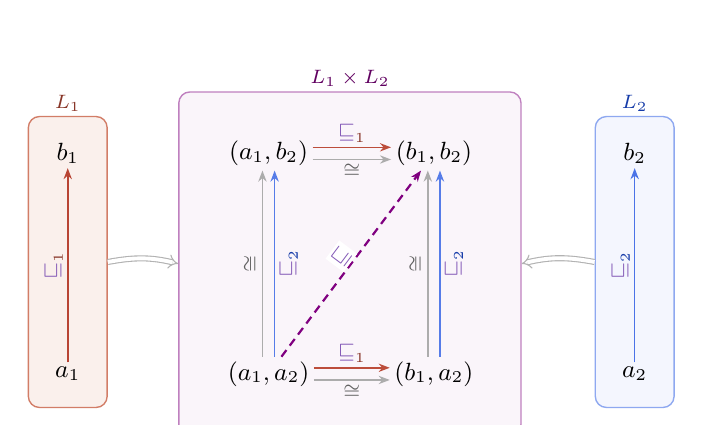
\begin{tikzpicture}[
    >={Stealth[length=4pt]},
    every node/.style={inner sep=1.5pt, font=\small},
    inducededge/.style={->, draw=Purple, dashed, line width=0.8pt, dash pattern=on 3pt off 2pt}
]
\node (b1) at (-3.6, 1.4) {$b_1$};
\node (a1) at (-3.6, -1.4) {$a_1$};
\draw[->, Mahogany!80, line width=0.55pt] (a1) -- node[auto, sloped, font=\scriptsize, Mahogany!75!black] {$\sqsubseteq_1$} (b1);

\node (b2) at ( 3.6, 1.4) {$b_2$};
\node (a2) at ( 3.6, -1.4) {$a_2$};
\draw[->, NavyBlue!80, line width=0.55pt] (a2) -- node[auto, sloped, font=\scriptsize, NavyBlue!75!black] {$\sqsubseteq_2$} (b2);

\node (aa) at (-1.05, -1.4) {$(a_1, a_2)$};
\node (ba) at ( 1.05, -1.4) {$(b_1, a_2)$};
\node (ab) at (-1.05,  1.4) {$(a_1, b_2)$};
\node (bb) at ( 1.05,  1.4) {$(b_1, b_2)$};

\draw[->, gray!65, line width=0.55pt, transform canvas={yshift=-2.2pt}]
    (aa) -- node[below, font=\scriptsize, gray!75!black] {$\cong$} (ba);
\draw[->, Mahogany!75, line width=0.55pt, transform canvas={yshift=2.2pt}]
    (aa) -- node[above, font=\scriptsize, Mahogany!75!black] {$\sqsubseteq_1$} (ba);

\draw[->, gray!65, line width=0.55pt, transform canvas={yshift=-2.2pt}]
    (ab) -- node[below, font=\scriptsize, gray!75!black] {$\cong$} (bb);
\draw[->, Mahogany!75, line width=0.55pt, transform canvas={yshift=2.2pt}]
    (ab) -- node[above, font=\scriptsize, Mahogany!75!black] {$\sqsubseteq_1$} (bb);

\draw[->, gray!65, line width=0.55pt, transform canvas={xshift=-2.2pt}]
    (aa) -- node[auto, sloped, font=\scriptsize, gray!75!black] {$\cong$} (ab);
\draw[->, NavyBlue!75, line width=0.55pt, transform canvas={xshift=2.2pt}]
    (aa) -- node[auto, sloped, swap, font=\scriptsize, NavyBlue!75!black] {$\sqsubseteq_2$} (ab);

\draw[->, gray!65, line width=0.55pt, transform canvas={xshift=-2.2pt}]
    (ba) -- node[auto, sloped, font=\scriptsize, gray!75!black] {$\cong$} (bb);
\draw[->, NavyBlue!75, line width=0.55pt, transform canvas={xshift=2.2pt}]
    (ba) -- node[auto, sloped, swap, font=\scriptsize, NavyBlue!75!black] {$\sqsubseteq_2$} (bb);

\draw[inducededge] (aa) -- node[sloped, above, font=\scriptsize, Purple, fill=white, inner sep=1pt] {$\sqsubseteq$} (bb);

\begin{scope}[on background layer]
  \node[draw=Mahogany!50, fill=Mahogany!5, rounded corners=4pt, line width=0.5pt,
        inner sep=8pt, fit={(a1)(b1)},
        label={[font=\scriptsize\itshape, Mahogany!75!black]above:$L_1$}] (lat1) {};
  \node[draw=NavyBlue!50, fill=NavyBlue!5, rounded corners=4pt, line width=0.5pt,
        inner sep=8pt, fit={(a2)(b2)},
        label={[font=\scriptsize\itshape, NavyBlue!75!black]above:$L_2$}] (lat2) {};
  \node[draw=Purple!50, fill=Purple!4, rounded corners=4pt, line width=0.5pt,
        inner sep=16pt, fit={(aa)(bb)},
        label={[font=\scriptsize\itshape, Purple!75!black]above:$L_1 \times L_2$}] (latP) {};
\end{scope}

\draw[-{Implies[]}, double, double distance=1.4pt, gray!60, line width=0.4pt] (lat1.east) to[bend left=12] (latP.west);
\draw[-{Implies[]}, double, double distance=1.4pt, gray!60, line width=0.4pt] (lat2.west) to[bend right=12] (latP.east);

\end{tikzpicture}
\caption{Product Lattice Precision}
\label{fig:product-bifunctor}
\end{figure}

\subsection{Well-Foundedness, Monotonicity, and Fixed Points}
\label{sec:fixed-points}

A partial order $(L, \sqsubseteq)$ is \textit{well-founded} if it admits no infinite \textit{strictly} descending chain $x_0 \sqsupset x_1 \sqsupset x_2 \sqsupset \cdots$. This is immediate on finite sets: every chain is bounded by the finite cardinality $|L|$.

A function $f : L \to L$ is \textit{monotone} if $x \sqsubseteq y$ implies $f(x) \sqsubseteq f(y)$, and \textit{anti-monotone} if $x \sqsubseteq y$ implies $f(y) \sqsubseteq f(x)$.

\begin{lemma}[Monotonicity of co-Heyting subtraction]\label{lem:heyt-mono}
In a co-Heyting algebra $(L, \sqsubseteq, \sqcup, \heytingminus)$, the binary operation $\heytingminus$ is monotone in its first argument and anti-monotone in its second: for all $a, a', b, b' \in L$,
\[ a \sqsubseteq a' \;\Rightarrow\; a \heytingminus b \sqsubseteq a' \heytingminus b, \qquad b \sqsubseteq b' \;\Rightarrow\; a \heytingminus b' \sqsubseteq a \heytingminus b. \]
\end{lemma}

\begin{proof}
By the universal property of $\heytingminus$, $x \heytingminus y \sqsubseteq z \iff x \sqsubseteq y \sqcup z$.
\textit{First argument:} take $z = a' \heytingminus b$. Then $a' \sqsubseteq b \sqcup z$, so $a \sqsubseteq a' \sqsubseteq b \sqcup z$, giving $a \heytingminus b \sqsubseteq z = a' \heytingminus b$.
\textit{Second argument:} take $z = a \heytingminus b$. Then $a \sqsubseteq b \sqcup z \sqsubseteq b' \sqcup z$, giving $a \heytingminus b' \sqsubseteq z = a \heytingminus b$.
\end{proof}

\begin{theorem}[Kleene Fixed Point, finite case]\label{thm:kleene}
Let $(L, \sqsubseteq, \bot)$ be a finite partial order with bottom element $\bot$, and let $f : L \to L$ be monotone. Then $f$ has a least fixed point $\mu f = f^n(\bot)$ for some $n \leq |L|$.
\end{theorem}

\begin{proof}
The chain $\bot \sqsubseteq f(\bot) \sqsubseteq f^2(\bot) \sqsubseteq \cdots$ is ascending by monotonicity. Since $L$ is finite, this chain must stabilise: there is some $n \leq |L|$ with $f^n(\bot) = f^{n+1}(\bot)$. So $f^n(\bot)$ is a fixed point. Further, $f^n(\bot)$ is a least fixed point: let $x$ be any fixed point of $f$. We show $f^k(\bot) \sqsubseteq x$ by induction on $k$. Base: $\bot \sqsubseteq x$ since $\bot$ is the bottom. Step: $f^{k+1}(\bot) = f(f^k(\bot)) \sqsubseteq f(x) = x$ by monotonicity of $f$ and the induction hypothesis.
\end{proof}

\begin{figure}[t]
\centering
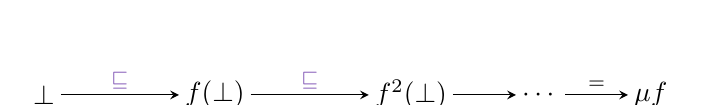
\begin{tikzpicture}[>=stealth, node distance=1.5cm, every node/.style={inner sep=2pt}]
  \node (b) {$\bot$};
  \node (f1) [right=of b] {$f(\bot)$};
  \node (f2) [right=of f1] {$f^2(\bot)$};
  \node (dots) [right=0.8cm of f2] {$\cdots$};
  \node (mu) [right=0.8cm of dots] {$\mu f$};
  \draw[->] (b) -- node[above,font=\scriptsize] {$\sqsubseteq$} (f1);
  \draw[->] (f1) -- node[above,font=\scriptsize] {$\sqsubseteq$} (f2);
  \draw[->] (f2) -- (dots);
  \draw[->] (dots) -- node[above,font=\scriptsize] {$=$} (mu);
\end{tikzpicture}
\caption{Kleene iteration to the least fixed point $\mu f$.}
\label{fig:kleene-iteration}
\end{figure}

%%% Local Variables:
%%% mode: LaTeX
%%% TeX-master: "PolymorphicTypeSlicing"
%%% End:

\section{The Core Calculus}
\label{sec:core-calculus}

\sectionlegend

In this chapter I present the core calculus which Type Slicing builds upon. It is a bidirectional, gradually typed lambda calculus based on the Hazel calculus~\cite{HazelLivePaper}, extended with products, sums, and explicit System~F polymorphism. Then, upon this, I define and prove several bi-Heyting lattices under a precision relation. 

\subsection{\yo Syntax \& Relations}
\label{sec:core-syntax}
\mechfile{Core/*/Base}

\begin{figure}[t]
\fbox{Syntax}\ \ \ Types $\tau$ and expressions $e$
\begin{align*}
\tau &::= \gap \mid * \mid \tau \Rightarrow \tau \mid \tau \times \tau \mid \tau + \tau \mid \forall\alpha.\;\tau \mid \alpha \\[4pt]
e &::= \gap \mid * \mid x \mid \lambda x \mathbin{:} \tau.\; e \mid \lambda x.\; e \mid e(e) \mid (e,\; e) \mid \pi_1\; e \mid \pi_2\; e \\
  &\quad\mid\; \iota_1\; e \mid \iota_2\; e \mid \mathbf{case}\;e\;\mathbf{of}\;x.\;e \mid y.\;e \mid \Lambda\alpha.\; e \mid e\langle\tau\rangle \mid \mathbf{let}\;x = e\;\mathbf{in}\;e
\end{align*}
\fbox{Derived forms}\ \ \ Definable in terms of the core syntax
\vspace{-0.5em}
\begin{align*}
(e : \tau) &\triangleq (\lambda x \mathbin{:} \tau.\; x)(e) &
\texttt{Bool} \triangleq * + * \\
\texttt{true} &\triangleq \iota_1\; * &
\texttt{false} \triangleq \iota_2\; * \\
\mathbf{if}\;e\;\mathbf{then}\;e_1\;\mathbf{else}\;e_2 &\triangleq \mathbf{case}\;e\;\mathbf{of}\;x.\;e_1 \mid y.\;e_2 & (x \notin \mathrm{FV}(e_1),\; y \notin \mathrm{FV}(e_2))
\end{align*}
\caption{Syntax of the core calculus. $\mathrm{FV}(\cdot)$ denotes the set of free variables of an expression.}
\label{fig:syntax}
\end{figure}

The syntax of the core calculus is given in Figure~\ref{fig:syntax}. The \textit{gap} type $\gap$ serves a dual role: in the gradual typing interpretation it is the dynamic type, and in the slicing interpretation it represents unrequired type information (to explain a query). Similarly a \gap in expressions represents omitted sub-expressions, irrelevant to the explanation resulting from a query. In type checking, omitted expressions synthesise the dynamic (omitted) type.

\subsubsection{\yo Consistency}
\mechfile{Core/Typ/\\Consistency}

\begin{figure}[t]
\fbox{$\tau_1 \sim \tau_2$}\ \ \ $\tau_1$ is consistent with $\tau_2$
\[\inference[$\sim\gap_1$]{}{\tau \sim \gap} \qquad
  \inference[$\sim\gap_2$]{}{\gap \sim \tau} \qquad
  \inference[$\sim{*}$]{}{* \sim *} \qquad
  \inference[$\sim{\Rightarrow}$]{\tau_1 \sim \tau_1' & \tau_2 \sim \tau_2'}{\tau_1 \Rightarrow \tau_2 \sim \tau_1' \Rightarrow \tau_2'}\]
\[\inference[$\sim{\times}$]{\tau_1 \sim \tau_1' & \tau_2 \sim \tau_2'}{\tau_1 \times \tau_2 \sim \tau_1' \times \tau_2'} \qquad
  \inference[$\sim{+}$]{\tau_1 \sim \tau_1' & \tau_2 \sim \tau_2'}{\tau_1 + \tau_2 \sim \tau_1' + \tau_2'} \qquad
  \inference[$\sim{\forall}$]{\tau \sim \tau'}{\forall\alpha.\;\tau \sim \forall\alpha.\;\tau'}\]
\caption{Type consistency.}
\label{fig:consistency}
\end{figure}

Type consistency (Figure~\ref{fig:consistency}) is exactly as presented in standard gradual type systems (\cref{sec:gradual-types}). That is, a weakening of equality, where every type is consistent with $\gap$, and compound types are consistent when their components are. Consistency is reflexive and symmetric but \textit{not} transitive.

\subsubsection{\yo Precision}
\mechfile{Core/*/\\Precision}

\begin{figure}[t]
\fbox{$\tau \sqsubseteq \tau'$}\ \ \ $\tau$ is less precise than $\tau'$
\[\inference[$\sqsubseteq\gap$]{}{\gap \sqsubseteq \tau} \qquad
  \inference[$\sqsubseteq{*}$]{}{* \sqsubseteq *} \qquad
  \inference[$\sqsubseteq{\alpha}$]{}{\alpha \sqsubseteq \alpha} \qquad
  \inference[$\sqsubseteq{\Rightarrow}$]{\tau_1 \sqsubseteq \tau_1' & \tau_2 \sqsubseteq \tau_2'}{\tau_1 \Rightarrow \tau_2 \sqsubseteq \tau_1' \Rightarrow \tau_2'}\]
\[\inference[$\sqsubseteq{\times}$]{\tau_1 \sqsubseteq \tau_1' & \tau_2 \sqsubseteq \tau_2'}{\tau_1 \times \tau_2 \sqsubseteq \tau_1' \times \tau_2'} \qquad
  \inference[$\sqsubseteq{+}$]{\tau_1 \sqsubseteq \tau_1' & \tau_2 \sqsubseteq \tau_2'}{\tau_1 + \tau_2 \sqsubseteq \tau_1' + \tau_2'} \qquad
  \inference[$\sqsubseteq{\forall}$]{\tau \sqsubseteq \tau'}{\forall\alpha.\;\tau \sqsubseteq \forall\alpha.\;\tau'}\]
\caption{Type precision.}
\label{fig:precision}
\end{figure}

Precision (Figure~\ref{fig:precision}) is a partial order that organises terms by \textit{information content}: for types, $\tau' \sqsubseteq \tau$ means $\tau$ has at least as much type information as $\tau'$. Here, $\gap$ is the global minimum. Expression precision is defined analogously. Figure~\ref{fig:term-precision-lattice} illustrates this with a small example.

\begin{figure}[t]
\centering
\begin{tikzpicture}[node distance=1.6cm, >=stealth, every node/.style={inner sep=2pt},
                    precarrow/.style={->, latticecolor!75, line width=0.5pt}]
  \node (top) {$\lambda x \mathbin{:} *.\; x$};
  \node (l)   [below left=1.4cm and 0.6cm of top] {$\lambda x \mathbin{:} *.\; \gap$};
  \node (r)   [below right=1.4cm and 0.6cm of top] {$\lambda x \mathbin{:} \gap.\; x$};
  \node (mid) [below=2.8cm of top] {$\lambda x \mathbin{:} \gap.\; \gap$};
  \node (bot) [below=1.4cm of mid] {$\gap$};
  \draw[precarrow] (l)   -- node[auto,sloped,font=\scriptsize] {$\sqsubseteq$} (top);
  \draw[precarrow] (r)   -- node[auto,sloped,font=\scriptsize] {$\sqsupseteq$} (top);
  \draw[precarrow] (mid) -- node[auto,sloped,font=\scriptsize] {$\sqsupseteq$} (l);
  \draw[precarrow] (mid) -- node[auto,sloped,font=\scriptsize] {$\sqsubseteq$} (r);
  \draw[precarrow] (bot) -- node[auto,sloped,font=\scriptsize] {$\sqsubseteq$} (mid);
\end{tikzpicture}
\caption{Hasse diagram of slices less precise than $\lambda x{:}*.\; x$, with each edge directed from a less-precise slice up to a more-precise slice.}
\label{fig:term-precision-lattice}
\end{figure}

\paragraph{Precision on assumptions.}\mechfile{Core/Assms/} In this calculus, I represent typing assumptions as \textit{finite} partial functions from variable names to types, with domain $\mathrm{dom}(\Gamma)$. Precision is defined by domain inclusion and pointwise precision on types in the (smaller) domain:
\[\gamma_1 \sqsubseteq \gamma_2 \iff \mathrm{dom}(\gamma_1) \subseteq \mathrm{dom}(\gamma_2) \text{ and } \gamma_1(x) \sqsubseteq \gamma_2(x) \text{ for all } x \in \mathrm{dom}(\gamma_1)\]
That is, a less precise type assumptions set either assumes fewer variables' types, or assumes less precise types on the present variables.

\begin{remark}[Mechanisation of assumptions]\label{rem:assms-mechanisation}
In the Agda mechanisation, assumptions are fixed-length lists indexed by de Bruijn position. An unused variable at position $i$ is represented by $\gap$ at that position. This is less general as we lose the ability to distinguish an `unused' variable from a `dynamic-typed' variable, but this distinction is never required. The partial-function presentation is more intuitive exposition.
\end{remark}

\begin{proposition}[\no Downward Well-Foundedness of Precision]\label{prop:precision-wf}
The strict precision ordering $\sqsubset$ is downward well-founded on types, expressions, and assumptions. Each family has a bottom element under precision:
\begin{itemize}
\item Types and expressions: $\bot = \gap$.
\item Assumptions: $\bot = \emptyset$.
\end{itemize}
\end{proposition}

\begin{proof}
Each object is a finite tree over a finite alphabet of constructors. A strict descent in precision must replace at least one non-$\gap$ position with $\gap$, as illustrated in Figure~\ref{fig:wf-tree}. Since there are finitely many positions, any descending chain has length bounded by the number of positions in the original term. And for assumptions, the finiteness of $\mathrm{dom}(\Gamma)$ bounds the number of variables available.
\end{proof}

\begin{figure}[t]
\centering
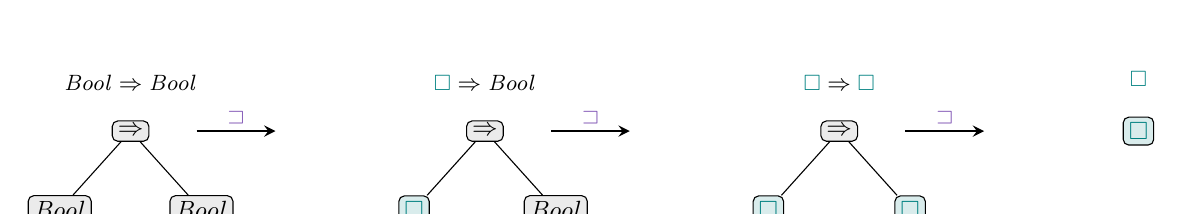
\begin{tikzpicture}[>=stealth, level distance=1cm, sibling distance=1.8cm,
    every node/.style={inner sep=2pt, font=\small},
    concrete/.style={draw, rounded corners=2pt, fill=black!8},
    gapped/.style={draw, rounded corners=2pt, fill=teal!15}]
  \node[concrete] (r1) {$\Rightarrow$}
    child {node[concrete] (l1) {$\mathit{Bool}$}}
    child {node[concrete] (r1r) {$\mathit{Bool}$}};
  \node[above=0.3cm of r1, font=\footnotesize] {$\mathit{Bool} \Rightarrow \mathit{Bool}$};

  \node[right=1.2cm of r1] (a1) {};
  \draw[->, thick] ([xshift=0.6cm]r1.east) -- node[above, font=\scriptsize] {$\sqsupset$} ++(1cm,0);

  \begin{scope}[xshift=4.5cm]
  \node[concrete] (r2) {$\Rightarrow$}
    child {node[gapped] (l2) {$\gap$}}
    child {node[concrete] (r2r) {$\mathit{Bool}$}};
  \node[above=0.3cm of r2, font=\footnotesize] {$\gap \Rightarrow \mathit{Bool}$};
  \end{scope}

  \draw[->, thick] ([xshift=0.6cm]r2.east) -- node[above, font=\scriptsize] {$\sqsupset$} ++(1cm,0);

  \begin{scope}[xshift=9cm]
  \node[concrete] (r3) {$\Rightarrow$}
    child {node[gapped] (l3) {$\gap$}}
    child {node[gapped] (r3r) {$\gap$}};
  \node[above=0.3cm of r3, font=\footnotesize] {$\gap \Rightarrow \gap$};
  \end{scope}

  \draw[->, thick] ([xshift=0.6cm]r3.east) -- node[above, font=\scriptsize] {$\sqsupset$} ++(1cm,0);

  \begin{scope}[xshift=12.8cm]
  \node[gapped] (bot) {$\gap$};
  \node[above=0.3cm of bot, font=\footnotesize] {$\gap$};
  \end{scope}
\end{tikzpicture}
\caption{A maximal descending chain in $\lfloor\mathit{Bool} \Rightarrow \mathit{Bool}\rfloor$.}
\label{fig:wf-tree}
\end{figure}

\subsection{\yo Lattice Properties}
\label{sec:core-lattice}
\mechfile{Core/*/\\Lattice}

\subsubsection{\yo Meets and Joins}
\label{sec:core-meets-joins}

The \textit{meet} $\tau_1 \sqcap \tau_2$ is the greatest lower bound (GLB) of two types under precision. It is defined inductively: types of the same `kind'\footnote{Top level type constructor} take meets of their components, and $\gap$ is an \textit{annihilator} ($\gap \sqcap \tau = \gap$). The meet is \textit{always} defined: when the outermost kinds differ, $\tau_1 \sqcap \tau_2 = \gap$ is a valid (and greatest) lower bound. Since all all pairs have a meet, we have that types form a \textit{meet-semilattice} with lower bound \gap (Section~\ref{sec:lattice-background}). Expression meet is defined analogously. Assumption meets are defined pointwise and by intersecting the domains.

The \textit{join} $\tau_1 \sqcup \tau_2$ is the least upper bound (LUB). It is similarly defined inductively and componentwise, but with $\gap$ acting as the \textit{identity} ($\gap \sqcup \tau = \tau$, $\tau \sqcup \gap = \tau$). However, unlike meets, the join is only defined for consistent types (i.e. types of the same kind): when $\tau_1$ and $\tau_2$ have different kinds, no upper bound exists.

\begin{remark}
One might hope to quotient types by consistency and form a join-semilattice. But, this fails because consistency is \textit{not transitive}: $\mathit{Int} \sim \gap \sim \texttt{Bool}$ does not imply $\mathit{Int} \sim \texttt{Bool}$.
\end{remark}

\subsubsection{\yo The Slice Lattice}
\label{sec:slice-lattice}
\mechfile{Core/Instances}

For a fixed type $\tau$, the \textit{slice lattice} of $\tau$ is the \textit{lower set} under precision:
\[\lfloor\tau\rfloor \;=\; \{\,\upsilon \mid \upsilon \sqsubseteq \tau\,\}\]
$\lfloor e \rfloor$, $\lfloor \C \rfloor$, and $\lfloor \Gamma \rfloor$ are defined analogously for expressions, contexts, and assumptions. Each slice lattice has top $\top = \tau$ and bottom $\bot = \gap$. Then precision, meets, and joins are simply lift unchanged into the slice lattice. Importantly all terms in the slice lattice are consistent, so joins are always defined:

\begin{lemma}[\yo Slices are Mutually Consistent]\label{lem:slices-consistent}
\mechfile{Core/Typ/\\Precision}
If\/ $\upsilon_1 \sqsubseteq \tau$ and $\upsilon_2 \sqsubseteq \tau$, then $\upsilon_1 \sim \upsilon_2$.
\end{lemma}

Hence, these slice lattices are \textit{bounded lattice}. We also get that the lattice is \textit{distributive}. And, they are on finite lattices:

\begin{theorem}[\no Slice Lattices are Finite]\label{thm:slice-finite}
Each slice lattice $\lfloor\tau\rfloor$, $\lfloor e \rfloor$, $\lfloor \C \rfloor$, and $\lfloor \Gamma \rfloor$ is finite. For a term with $n$ positions, the slice lattice has at most $2^n$ elements.
\end{theorem}

Every finite distributive lattice is a bi-Heyting algebra~\cite{DaveyPriestley}, so the slice lattices are bi-Heyting: in a finite lattice the implication and subtraction operations below can be defined directly as a finite join / meet, respectively.

\mechfile{Core/*/Lattice}
\begin{majortheorembox}
\mechbox{typ-slice-\\BiHeyting}%
\begin{theorem}[\po Slice Lattices are Bounded Distributive Bi-Heyting Algebras]\label{thm:slice-lattices}
Each slice lattice $\lfloor\tau\rfloor$, $\lfloor e \rfloor$, $\lfloor \C \rfloor$, and $\lfloor \Gamma \rfloor$ is a bounded distributive bi-Heyting algebra:
\begin{itemize}
\item \yo \textbf{Bounded}: bottom $\bot = \gap$ (or $\emptyset$ for assumptions), top $\top = \tau$ (or $e$, $\C$, $\Gamma$).
\item \yo \textbf{Distributive}: meet distributes over join, $\upsilon_1 \sqcap (\upsilon_2 \sqcup \upsilon_3) = (\upsilon_1 \sqcap \upsilon_2) \sqcup (\upsilon_1 \sqcap \upsilon_3)$ (and dually).
\item \textbf{Bi-Heyting}: equipped with
\begin{itemize}
\item \po \textbf{Implication}: $\upsilon_1 \to \upsilon_2 = \bigsqcup\{\,\upsilon \mid \upsilon \sqcap \upsilon_1 \sqsubseteq \upsilon_2\,\}$ --- the most precise slice compatible with refining $\upsilon_1$ to at most $\upsilon_2$;
\item \po \textbf{Subtraction}: $\upsilon_1 \setminus \upsilon_2 = \bigsqcap\{\,\upsilon \mid \upsilon_1 \sqsubseteq \upsilon_2 \sqcup \upsilon\,\}$ --- the least precise slice whose join with $\upsilon_2$ recovers $\upsilon_1$.
\end{itemize}
\end{itemize}
\end{theorem}
\end{majortheorembox}

\paragraph{Inductive Definition:} Of course, calculating those joins / meets directly is very inefficient. We can define both inductively on slice lattices of the sub-terms, as demonstrated by example below for the lattice $\lfloor \tau_1 \Rightarrow \tau_2 \rfloor$ (inductively on $\lfloor \tau_1 \rfloor$ and $\lfloor \tau_2 \rfloor$).

\begin{itemize}

\item \textit{Implication} $\cdot \heytingto \cdot$
\begin{align*}
\gap \heytingto \upsilon \;&=\; \top \\
\upsilon \heytingto \gap \;&=\; \gap && \text{(when $\upsilon \sqsupset \gap$)} \\
{*} \heytingto {*} \;&=\; {*}\\
(\upsilon_1 \Rightarrow \upsilon_2) \heytingto (\upsilon_1' \Rightarrow \upsilon_2') \;&=\; (\upsilon_1 \heytingto \upsilon_1') \Rightarrow (\upsilon_2 \heytingto \upsilon_2')
\end{align*}

\item \textit{Subtraction} $\cdot \heytingminus \cdot$
\begin{align*}
\gap \heytingminus \upsilon \;&=\; \gap \\
\upsilon \heytingminus \gap \;&=\; \upsilon \\
{*} \heytingminus {*} \;&=\; \gap\\
  (\upsilon_1 \Rightarrow \upsilon_2) \heytingminus (\upsilon_1' \Rightarrow \upsilon_2') \;&=\; \begin{cases} \gap & \text{if $\upsilon_1 \heytingminus \upsilon_1' = \gap$ and $\upsilon_2 \heytingminus \upsilon_2' = \gap$} \\
    (\upsilon_1 \heytingminus \upsilon_1') \Rightarrow (\upsilon_2 \heytingminus \upsilon_2') & \text{otherwise} \end{cases}
\end{align*}
\end{itemize}

\begin{remark}[Mechanisation of Bi-Heyting operators]\label{rem:lattice-mechanisation}
The implication and subtraction are only fully mechanised for the type-slice lattice $\lfloor\tau\rfloor$, which is the only lattice for which they are actually \emph{used} in the forthcoming calculi.
\end{remark}

\paragraph{Notation: Slice Lattices as Highlighted Terms.} An element of a slice lattice can be notated as the original (top) term with omitted regions (replaced by a \gap) left unhighlighted and kept regions highlighted. For instance, the slice $\mathit{Int} \Rightarrow \gap$ in $\lfloor\mathit{Int} \Rightarrow \mathit{Bool}\rfloor$ can be represented as $\sli{\mathit{Int} \Rightarrow}\, \mathit{Bool}$.

The lattice operations have direct visual interpretations with this notation: meet $\sqcap$ is the intersection of highlighted regions, join $\sqcup$ is the union, implication $\heytingto$ is the largest piece compatible with the target, and subtraction $\heytingminus$ is the smallest piece recovering the source. Worked on $\lfloor (* \Rightarrow *) \times * \rfloor$ --- a pair of a function and a base value:
\begin{center}
\begin{tabular}{r@{\;}l}
$\sli{(* \Rightarrow *) \times}\, * \;\;\sqcap\;\; (* \Rightarrow *) \sli{\times *}$ & $=\;\; (* \Rightarrow *) \sli{\times}\, *$\\
$\sli{(* \Rightarrow *) \times}\, * \;\;\sqcup\;\; (* \Rightarrow *) \sli{\times *}$ & $=\;\; \sli{(* \Rightarrow *) \times *}$\\
$\sli{(* \Rightarrow *) \times}\, * \;\;\heytingto\;\; \sli{(* \Rightarrow}\, *\sli{) \times *}$ & $=\;\; \sli{(* \Rightarrow}\, *\sli{) \times *}$\\
$\sli{(* \Rightarrow *) \times} * \;\;\heytingminus\;\; \sli{(* \Rightarrow}\, *\sli{) \times *}$ & $=\;\; (\, *\, \sli{\Rightarrow *) \times}\, *$\\
\end{tabular}
\end{center}

\paragraph{No Boolean Lattice.} The pseudo-complement $\neg\upsilon = \upsilon \heytingto \gap$ and the supplement ${\sim}\upsilon = \top \heytingminus \upsilon$ do \emph{not} coincide on slice lattices, so they are not Boolean algebras. Take $\upsilon = \sli{* \Rightarrow}\, *$ in $\lfloor * \Rightarrow * \rfloor$:
\begin{align*}
\neg\upsilon \;&=\; \sli{* \Rightarrow}\, * \;\heytingto\; * \Rightarrow * \;=\; * \Rightarrow *, \\
{\sim}\upsilon \;&=\; \sli{* \Rightarrow *} \;\heytingminus\; \sli{* \Rightarrow}\, * \;=\; *\, \sli{\Rightarrow *}.
\end{align*}
The two disagree ($* \Rightarrow * \neq *\,\sli{\Rightarrow *}$). Consequentially, the Boolean complementation laws fail on either side: the Law of the Excluded Middle fails for pseudo-negation, and the Principle of Contradiction fails for the supplement:
\[\upsilon \;\sqcup\; \neg\upsilon \;=\; \sli{* \Rightarrow}\, * \;\sqcup\; * \Rightarrow * \;=\; \sli{* \Rightarrow}\, * \;\neq\; \sli{* \Rightarrow *}\]\[
  \upsilon \;\sqcap\; {\sim}\upsilon \;=\; \sli{* \Rightarrow}\, * \;\sqcap\; *\, \sli{\Rightarrow *} \;=\; *\, \sli{\Rightarrow}\, * \;\neq\; * \Rightarrow *.\]

\subsubsection{\no Well-Foundedness of Slice Lattices}
\label{sec:slice-wf}

\begin{proposition}[\no Upward Well-Foundedness of Slice Lattices]\label{prop:slice-wf-up}
For each of the four families, the reversed strict precision ordering $\sqsupseteq$ on $\lfloor\cdot\rfloor$ is well-founded.
\end{proposition}

\begin{proof}
Each slice lattice is finite (Theorem~\ref{thm:slice-finite}). A finite poset with a top element admits no infinite ascending chains.
\end{proof}

Combined with downwards well-foundedness (Proposition~\ref{prop:precision-wf}), this gives well-foundedness in both directions within each slice.

\subsection{\yo Typing Rules}
\label{sec:core-typing}
\mechfile{Semantics/Statics/\\Typing}

\begin{figure}[p]
\small
\fbox{$\synthesis{e}{\tau}$}\ \ \ $e$ synthesises type $\tau$ under type variable context $\Delta$ and typing assumptions $\Gamma$
\[\inference[\synr{$\gap$}]{}{\synthesis{\gap}{\gap}} \qquad
  \inference[\synr{*}]{}{\synthesis{*}{*}}\]
\[\inference[\synr{Var}]{x : \tau \in \Gamma}{\synthesis{x}{\tau}}\]
\[\inference[\synr{$\lambda$Ann}]{\wf{\tau_1} & \synthesis[\Delta;\,\Gamma, x \mathbin{:} \tau_1]{e}{\tau_2}}{\synthesis{\lambda x \mathbin{:} \tau_1.\; e}{\tau_1 \Rightarrow \tau_2}} \qquad
  \inference[\synr{let}]{\synthesis{e_1}{\tau_1} & \synthesis[\Delta;\,\Gamma, x \mathbin{:} \tau_1]{e_2}{\tau_2}}{\synthesis{\mathbf{let}\;x = e_1\;\mathbf{in}\;e_2}{\tau_2}}\]
\[\inference[\synr{$\Lambda$}]{\synthesis[\Delta, \alpha;\,\Gamma]{e}{\tau}}{\synthesis{\Lambda\alpha.\; e}{\forall\alpha.\;\tau}} \qquad
  \inference[\synr{TApp}]{\wf{\sigma} & \synthesis{e}{\tau} & \tau \sqcup \forall\alpha.\;\gap \equiv \forall\alpha.\;\tau'}{\synthesis{e\langle\sigma\rangle}{[\alpha \mapsto \sigma]\,\tau'}}\]
\[\inference[\synr{App}]{\synthesis{e_1}{\tau} & \tau \sqcup (\gap \Rightarrow \gap) \equiv \tau_1 \Rightarrow \tau_2 & \analysis{e_2}{\tau_1}}{\synthesis{e_1(e_2)}{\tau_2}}\]
\[\inference[\synr{\&}]{\synthesis{e_1}{\tau_1} & \synthesis{e_2}{\tau_2}}{\synthesis{(e_1,\; e_2)}{\tau_1 \times \tau_2}}\]
\[\inference[\synr{$\pi_1$}]{\synthesis{e}{\tau} & \tau \sqcup (\gap \times \gap) \equiv \tau_1 \times \tau_2}{\synthesis{\pi_1\; e}{\tau_1}} \qquad
  \inference[\synr{$\pi_2$}]{\synthesis{e}{\tau} & \tau \sqcup (\gap \times \gap) \equiv \tau_1 \times \tau_2}{\synthesis{\pi_2\; e}{\tau_2}}\]
\[\inference[\synr{case}]{\synthesis{e}{\tau} & \tau \sqcup (\gap + \gap) \equiv \tau_1 + \tau_2 & \tau_1' \sim \tau_2' \\ \synthesis[\Delta;\,\Gamma, x \mathbin{:} \tau_1]{e_1}{\tau_1'} & \synthesis[\Delta;\,\Gamma, y \mathbin{:} \tau_2]{e_2}{\tau_2'}}{\synthesis{\mathbf{case}\;e\;\mathbf{of}\;x.\;e_1 \mid y.\;e_2}{\tau_1' \sqcup \tau_2'}}\]
\caption{Synthesis rules.}
\label{fig:synthesis-rules}
\end{figure}

\begin{figure}[p]
\small
\fbox{$\analysis{e}{\tau}$}\ \ \ $e$ analyses against type $\tau$ under $\Delta$ and $\Gamma$
\[\inference[\anar{Sub}]{\synthesis{e}{\tau'} & \tau \sim \tau'}{\analysis{e}{\tau}}\]
\[\inference[\anar{$\lambda$}]{\tau \sqcup (\gap \Rightarrow \gap) \equiv \tau_1 \Rightarrow \tau_2 & \analysis[\Delta;\,\Gamma, x \mathbin{:} \tau_1]{e}{\tau_2}}{\analysis{\lambda x.\; e}{\tau}}\]
\[\inference[\anar{$\lambda$Ann}]{\wf{\tau_1} & \tau \sim \tau_1 \Rightarrow \gap \\ \tau \sqcup \tau_1 \Rightarrow \gap \equiv \tau_1' \Rightarrow \tau_2 & \analysis[\Delta;\,\Gamma, x \mathbin{:} \tau_1]{e}{\tau_2}}{\analysis{\lambda x \mathbin{:} \tau_1.\; e}{\tau}}\]
\[\inference[\anar{case}]{\synthesis{e}{\tau'} & \tau' \sqcup (\gap + \gap) \equiv \tau_1 + \tau_2 \\ \analysis[\Delta;\,\Gamma, x \mathbin{:} \tau_1]{e_1}{\tau} & \analysis[\Delta;\,\Gamma, y \mathbin{:} \tau_2]{e_2}{\tau}}{\analysis{\mathbf{case}\;e\;\mathbf{of}\;x.\;e_1 \mid y.\;e_2}{\tau}}\]
\[\inference[\anar{$\iota_1$}]{\tau \sqcup (\gap + \gap) \equiv \tau_1 + \tau_2 & \analysis{e}{\tau_1}}{\analysis{\iota_1\; e}{\tau}} \qquad
  \inference[\anar{$\iota_2$}]{\tau \sqcup (\gap + \gap) \equiv \tau_1 + \tau_2 & \analysis{e}{\tau_2}}{\analysis{\iota_2\; e}{\tau}}\]
\[\inference[\anar{\&}]{\tau \sqcup (\gap \times \gap) \equiv \tau_1 \times \tau_2 & \analysis{e_1}{\tau_1} & \analysis{e_2}{\tau_2}}{\analysis{(e_1,\; e_2)}{\tau}}\]
\[\inference[\anar{let}]{\synthesis{e_1}{\tau_1} & \analysis[\Delta;\,\Gamma, x \mathbin{:} \tau_1]{e_2}{\tau}}{\analysis{\mathbf{let}\;x = e_1\;\mathbf{in}\;e_2}{\tau}}\]
\caption{Analysis rules. \anar{Sub} is the unique bridge from analysis to synthesis.}
\label{fig:analysis-rules}
\end{figure}

The complete bidirectional typing rules are given in Figures~\ref{fig:synthesis-rules} and~\ref{fig:analysis-rules}, where types may contain variables which must be within a type variable context $\Delta$. That is, a type $\tau$ is \textit{well-formed} under $\Delta$, written $\wf{\tau}$, if every free type variable in $\tau$ is a member of $\Delta$.

The rules are mostly standard, but I highlight notable differences in my presentation compared to the usual bidirectional systems:

\begin{itemize}
\item \textbf{Join-based matching}: Terms can synthesise $\gap$ which is not syntactically a function, but should be treated as such (it is consistent with the function type). We can extract the argument and return types with a join: $\tau \sqcup (\gap \Rightarrow \gap) \equiv \tau_1 \Rightarrow \tau_2$. Similarly for other compound types.\footnote{This is equivalent to the standard use of `matching functions' in the gradual typing literature, typically notated $\tau \blacktriangleright \tau_1 \Rightarrow \tau_2$.}

\item \textbf{Case expressions} can be type-checked in synthesis mode (\synr{case}), require the branch types $\tau_1$ and $\tau_2$ to be \textit{consistent}, synthesising the \textit{join} $\tau_1 \sqcup \tau_2$.

\item \textbf{Annotated vs.\ unannotated lambdas}: Annotated lambdas, $\lambda x \mathbin{:} \tau_1.\; e$, can synthesise their type using the annotation on the argument, while $\lambda x.\; e$ can only analyse as there is no way to determine the type of the argument at the definition site.

\item \textbf{Let bindings vs.\ annotated lambdas}: Unannotated let bindings, $\mathbf{let}\;x = e_1\;\mathbf{in}\;e_2$, \textit{synthesise} $e_1$ and binds the resulting type for $x$, whereas an annotated lambda application $(\lambda x \mathbin{:} \tau.\; e_2)(e_1)$ \textit{analyses} $e_1$ against $\tau$. 

Hence, annotated let bindings can be simulated by annotated lambdas, but unannotated let bindings cannot. An unannotated let binding can be conceptualised as a function application between an unannotated function and a argument but with type information flowing from argument into the function; therefore, a second application rule for unannotated lambdas is a more general formulation for unannotated let bindings. But this calculus make let bindings explicit for clarity.
\end{itemize}

\subsection{\yo Context Classification}
\label{sec:context-classification-section}
\mechfile{Core/Ctx/Base,\\Core/Ctx/Precision,\\Semantics/Statics/\\CtxTyping}

Context classification is a novel construction for bidirectional type systems. It is inspired by one-hole contexts (zippers) of algebraic data types~\cite{Huet1997}, decomposing a data structure into a focused element and its surrounding context. I apply the same idea applies to \textit{typing derivations}: given a derivation of an expression $e$ and focusing on a sub-term $e'$ in $e$, the classification decomposes it into the \textit{surrounding context} (carrying all typing information \textit{outside} the focused sub-term $e'$) and the \textit{focused sub-derivation} (carrying all typing information from \textit{inside} the focused sub-term $e'$). 

The classification also records the extra assumptions made available at the focus by additional bound variables introduced in the captured context, and the mode of the focus (whether or not the sub-term synthesises a type). Both of these are necessary to allow type checking of the focus directly from the context classification derivation.

\begin{remark}
    This construction replaces and generalises the notion of \textit{checking contexts} from the previous type slicing theory.
\end{remark}

\subsubsection{\yo Context Syntax}
\label{sec:context-syntax}

\begin{figure}[t]
\fbox{Syntax}\ \ \ One-hole expression contexts $\C$
\begin{align*}
\C &::= \cmark \mid \lambda x \mathbin{:} \tau.\; \C \mid \lambda x.\; \C \mid \C(e) \mid e(\C) \mid \C\langle\tau\rangle \\
  &\quad\mid\; (\C,\; e) \mid (e,\; \C) \mid \iota_1\; \C \mid \iota_2\; \C \mid \pi_1\; \C \mid \pi_2\; \C \\
  &\quad\mid\; \mathbf{case}\;e\;\mathbf{of}\;x.\;\C \mid y.\;f \mid \mathbf{case}\;e\;\mathbf{of}\;x.\;f \mid y.\;\C \\
  &\quad\mid\; \Lambda\alpha.\; \C \mid \mathbf{let}\;x = \C\;\mathbf{in}\;e \mid \mathbf{let}\;x = e\;\mathbf{in}\;\C
\end{align*}
\fbox{$\C[e]$}\ \ \ Plug expression $e$ into the hole $\cmark$
\vspace{-0.5em}
\begin{align*}
\cmark[e] &= e \\
(\lambda x \mathbin{:} \tau.\; \C)[e] &= \lambda x \mathbin{:} \tau.\; \C[e] \\
(\C_1(e_2))[e] &= \C_1[e](e_2) \qquad\qquad \text{(similarly for all other constructors)}
\end{align*}
\fbox{$\gap_\C$}\ \ \ Purely structural context: replace all sub-terms with $\gap$, preserving structure
\vspace{-0.5em}
\begin{align*}
\gap_\cmark &= \cmark &
\gap_{\lambda x \mathbin{:} \tau.\; \C} &= \lambda x \mathbin{:} \gap.\; \gap_\C &
\gap_{\C(e)} &= \gap_\C(\gap) \quad \text{etc.}
\end{align*}
\caption{One-hole expression contexts. $\cmark$ marks the hole; $\C[e]$ plugs it.}
\label{fig:contexts}
\end{figure}

First, I define one-hole contexts on terms in Figure~\ref{fig:contexts}. The focus of the context is notated $\cmark$ and is restricted to a single position in an expression.

\subsubsection{\yo Context Precision and Plugging Contexts}
\label{sec:context-precision}
Then, for any context, you can substitute a term into the focus to produce a complete term. This is notated by $\C[e]$, plugging $e$ into context $\C$.

Precision on contexts, $\C' \sqsubseteq \C$, requires the two contexts to share the focus in the same structural position, with componentwise precision on sub-terms and sub-contexts. Within each slice lattice $\lfloor\C\rfloor$ (Section~\ref{sec:slice-lattice}), the bottom is the \textit{purely structural context} $\gap_\C$: all sub-terms omitted, preserving only the focus location (Figure~\ref{fig:contexts}). 

Downwards well-foundedness holds within each $\lfloor\C\rfloor$ by the same argument as Proposition~\ref{prop:precision-wf}.

Importantly, context plugging preserves precision:

\begin{lemma}[\yo Plug Preserves Precision]\label{lem:plug-precision}
If\/ $\C' \sqsubseteq \C$ and $e' \sqsubseteq e$, then $\C'[e]' \sqsubseteq \C[e]$. (Figure~\ref{fig:plug-precision})
\end{lemma}

This allows slicing to independently slice the \textit{external} type information from the context and the \textit{internal} type information of the focused term independently, while ensure the whole program slice (plugging the two together) remains a valid slice of the original program.

\begin{figure}[t]
\centering
\begin{tikzcd}[column sep=large, row sep=large]
(\C,\; e) \arrow[r, "\text{plug}"] & \C[e] \\
{\color{assumed} (\C',\; e')} \arrow[u, assumed, "\sqsubseteq" {sloped}] \arrow[r, "\text{plug}"'] & \C'[e'] \arrow[u, dashed, induced, "\sqsubseteq" {sloped}]
\end{tikzcd}
\caption{Plug preserves precision (Lemma~\ref{lem:plug-precision}).}
\label{fig:plug-precision}
\end{figure}

\subsubsection{\yo The Classification Judgement}
\label{sec:context-classification}

The context classification judgement is notated:
\[\ctxclass{\C}{d}{\Gamma'}{m}\]
reading as: ``under type variable context $\Delta$ and assumptions $\Gamma$, context $\C$ in a derivation of outer mode $d$ has its focus typed under $\Delta';\,\Gamma'$ in focus mode $m$''. 

The \textit{outer derivation mode} $d$ records whether the whole expression $\C[e]$ is in a synthesis derivation producing type $\tau$ ($d = {\color{BrickRed}\Uparrow}\;\tau$) or an analysis derivation against $\tau$ ($d = {\color{BlueViolet}\Downarrow}\;\tau$). The \textit{focus mode} $m$ records what the focus $e$ must satisfy: either $m = {\color{BrickRed}\Rightarrow}\;\tau'$ (the focus must synthesise type $\tau'$) or $m = {\color{BlueViolet}\Leftarrow}\;\tau'$ (the focus must analyse against $\tau'$). Both the outer derivation mode and focus mode carry a type, enabling the classification to track type flow through the derivation.

Further, we record the \textit{focus assumptions} $\Gamma'$ and the \textit{focus mode} $m$ as mentioned previously. Finally, several rule require \textit{extra premises} which systematically match with the premises of the typing rule that each context classification rule represents.

\paragraph{Example.} Consider the derivation of $\synthesis{e_1(e_2)}{\tau_2}$ via \synr{App}, where $\synthesis{e_1}{\tau}$, $\tau \sqcup (\gap \Rightarrow \gap) \equiv \tau_1 \Rightarrow \tau_2$, and $\analysis{e_2}{\tau_1}$.
\begin{itemize}
\item \textbf{Function position} ($e_1$ is the focus, $\C = \cmark(e_2)$): The corresponding classification is: $\ctxclass{\cmark(e_2)}{{\color{BrickRed}\Uparrow}\;\tau_2}{\Delta;\,\Gamma}{{\color{BrickRed}\Rightarrow}\;\tau}$. The focus must synthesise type $\tau$ as per the focus mode, with the extra premises being $\tau \sqcup (\gap \Rightarrow \gap) \equiv \tau_1 \Rightarrow \tau_2$ and $\analysis{e_2}{\tau_1}$.
\item \textbf{Argument position} ($e_2$ is the focus, $\C = e_1(\cmark)$): The corresponding classification is: $\ctxclass{e_1(\cmark)}{{\color{BrickRed}\Uparrow}\;\tau_2}{\Delta;\,\Gamma}{{\color{BlueViolet}\Leftarrow}\;\tau_1}$. The focus analyses against $\tau_1$ as per the focus mode, with the extra premises being: $\synthesis{e_1}{\tau}$ and $\tau \sqcup (\gap \Rightarrow \gap) \equiv \tau_1 \Rightarrow \tau_2$.
\end{itemize}

\begin{figure}[p]
\small
\fbox{$\ctxclass{\C}{d}{\Delta';\,\Gamma'}{m}$}\ \ \ Context $\C$ at outer derivation mode $d$ classifies its focus under $\Delta';\,\Gamma'$ in focus mode $m$

\bigskip
\fbox{Base cases}\ \ \ identity contexts (focus mode matches outer derivation mode):
\[\inference[\texttt{s$\cmark$}]{}{\ctxclass{\cmark}{{\color{BrickRed}\Uparrow}\;\tau}{\Delta;\,\Gamma}{{\color{BrickRed}\Rightarrow}\;\tau}} \qquad
  \inference[\texttt{a$\cmark$}]{}{\ctxclass{\cmark}{{\color{BlueViolet}\Downarrow}\;\tau}{\Delta;\,\Gamma}{{\color{BlueViolet}\Leftarrow}\;\tau}}\]

\medskip
\fbox{Synthesis mode: $d = {\color{BrickRed}\Uparrow}\;\tau$}\ \ \ the overall expression $\C[e]$ synthesises:
\[\inference[\texttt{s$\lambda$:}]{\wf{\tau_1} & \ctxclass[\Delta;\,\Gamma, x \mathbin{:} \tau_1]{\C}{{\color{BrickRed}\Uparrow}\;\tau_2}{\Delta';\,\Gamma'}{m}}{\ctxclass{\lambda x \mathbin{:} \tau_1.\;\C}{{\color{BrickRed}\Uparrow}\;\tau_1 \Rightarrow \tau_2}{\Delta';\,\Gamma'}{m}}\]
\[\inference[\texttt{s$\circ_1$}]{\ctxclass{\C}{{\color{BrickRed}\Uparrow}\;\tau}{\Delta';\,\Gamma'}{m} & \tau \sqcup (\gap \Rightarrow \gap) \equiv \tau_1 \Rightarrow \tau_2 & \analysis{e_2}{\tau_1}}{\ctxclass{\C(e_2)}{{\color{BrickRed}\Uparrow}\;\tau_2}{\Delta';\,\Gamma'}{m}}\]
\[\inference[\texttt{s$\circ_2$}]{\synthesis{e_1}{\tau} & \tau \sqcup (\gap \Rightarrow \gap) \equiv \tau_1 \Rightarrow \tau_2 & \ctxclass{\C}{{\color{BlueViolet}\Downarrow}\;\tau_1}{\Delta';\,\Gamma'}{m}}{\ctxclass{e_1(\C)}{{\color{BrickRed}\Uparrow}\;\tau_2}{\Delta';\,\Gamma'}{m}}\]
\[\inference[\texttt{s$\&_1$}]{\ctxclass{\C}{{\color{BrickRed}\Uparrow}\;\tau_1}{\Delta';\,\Gamma'}{m} & \synthesis{e_2}{\tau_2}}{\ctxclass{(\C,\; e_2)}{{\color{BrickRed}\Uparrow}\;\tau_1 \times \tau_2}{\Delta';\,\Gamma'}{m}}\]
\[\inference[\texttt{s$\Lambda$}]{\ctxclass[\Delta, \alpha;\,\Gamma]{\C}{{\color{BrickRed}\Uparrow}\;\tau}{\Delta';\,\Gamma'}{m}}{\ctxclass{\Lambda\alpha.\;\C}{{\color{BrickRed}\Uparrow}\;\forall\alpha.\;\tau}{\Delta';\,\Gamma'}{m}}\]
\[\inference[\texttt{sdef$_2$}]{\synthesis{e_1}{\tau'} & \ctxclass[\Delta;\,\Gamma, x \mathbin{:} \tau']{\C}{{\color{BrickRed}\Uparrow}\;\tau}{\Delta';\,\Gamma'}{m}}{\ctxclass{\mathbf{let}\;x = e_1\;\mathbf{in}\;\C}{{\color{BrickRed}\Uparrow}\;\tau}{\Delta';\,\Gamma'}{m}}\]

\medskip
\fbox{Analysis mode: $d = {\color{BlueViolet}\Downarrow}\;\tau$}\ \ \ the overall expression $\C[e]$ analyses:
\[\inference[\texttt{a$\lambda\Rightarrow$}]{\tau \sqcup (\gap \Rightarrow \gap) \equiv \tau_1 \Rightarrow \tau_2 & \ctxclass[\Delta;\,\Gamma, x \mathbin{:} \tau_1]{\C}{{\color{BlueViolet}\Downarrow}\;\tau_2}{\Delta';\,\Gamma'}{m}}{\ctxclass{\lambda x.\;\C}{{\color{BlueViolet}\Downarrow}\;\tau}{\Delta';\,\Gamma'}{m}}\]
\[\inference[\texttt{a$\iota_1$}]{\tau \sqcup (\gap + \gap) \equiv \tau_1 + \tau_2 & \ctxclass{\C}{{\color{BlueViolet}\Downarrow}\;\tau_1}{\Delta';\,\Gamma'}{m}}{\ctxclass{\iota_1\;\C}{{\color{BlueViolet}\Downarrow}\;\tau}{\Delta';\,\Gamma'}{m}}\]

\medskip
\fbox{Subsumption: ${\color{BrickRed}\Uparrow}\;\tau' \;\leadsto\; {\color{BlueViolet}\Downarrow}\;\tau$}\ \ \ the unique bridge from synthesis to analysis derivation mode:
\[\inference[\texttt{aSub}]{\ctxclass{\C}{{\color{BrickRed}\Uparrow}\;\tau'}{\Delta';\,\Gamma'}{m} & \tau \sim \tau'}{\ctxclass{\C}{{\color{BlueViolet}\Downarrow}\;\tau}{\Delta';\,\Gamma'}{m}}\]
\caption{Selected context classification rules.}
\label{fig:context-classification}
\end{figure}

I give a few representative rules of context classification in Figure~\ref{fig:context-classification}. The construction of these rules is systematic, one for each typing rule and focus position. The only exception being the identity contexts $\texttt{s}\cmark$ and $\texttt{a}\cmark$ (the base cases) saying that the focus mode must match the outer derivation mode.

Correctness of context classification is formalised via a \textit{totality} theorem: every well-typed expression can be decomposed into context and expression at some focus, with a context classification matching a (consistent) typing derivation of the focused term. Conversely, a \textit{soundness} theorem states that a valid classification and expression satisfying the focus typing mode can be composed into a well-typed plugged expression.

\begin{majortheorembox}
\mechbox{plug-decompose}%
\begin{theorem}[\yo Plug Decomposition -- Totality]\label{thm:plug-decomposition}
For any context $\C$, expression $e$, and outer derivation mode $d$:
\begin{itemize}
\item If\/ $\synthesis{\C[e]}{\tau}$, then there exist $\Delta'$, $\Gamma'$, and $m$ such that $\ctxclass{\C}{{\color{BrickRed}\Uparrow}\;\tau}{\Delta';\,\Gamma'}{m}$ and $e$ satisfies focus mode $m$ under $\Delta';\,\Gamma'$.
\item If\/ $\analysis{\C[e]}{\tau}$, then there exist $\Delta'$, $\Gamma'$, and $m$ such that $\ctxclass{\C}{{\color{BlueViolet}\Downarrow}\;\tau}{\Delta';\,\Gamma'}{m}$ and $e$ satisfies focus mode $m$ under $\Delta';\,\Gamma'$.
\end{itemize}
Here ``$e$ satisfies focus mode $m$ under $\Delta';\,\Gamma'$'' means: if $m = {\color{BrickRed}\Rightarrow}\;\tau'$ then $\Delta';\,\Gamma' \vdash e\;{\color{BrickRed}\Uparrow}\;\tau'$; if $m = {\color{BlueViolet}\Leftarrow}\;\tau'$ then $\Delta';\,\Gamma' \vdash e\;{\color{BlueViolet}\Downarrow}\;\tau'$.
\end{theorem}
\end{majortheorembox}

\begin{majortheorembox}
\mechbox{plug-compose}%
\begin{theorem}[\yo Plug Composition -- Soundness]\label{thm:plug-composition}
For any context $\C$, expression $e$, outer derivation mode $d$, and focus mode $m$: if\/ $\ctxclass{\C}{d}{\Delta';\,\Gamma'}{m}$ and $e$ satisfies focus mode $m$ under $\Delta';\,\Gamma'$, then $\C[e]$ satisfies outer derivation mode $d$ under $\Delta;\,\Gamma$.
\end{theorem}
\end{majortheorembox}

\subsection{\yo Metatheory: Graduality \& Unicity}
\label{sec:core-metatheory}
\mechfile{Semantics/\\Graduality}

Finally, the static gradual guarantee (\cref{sec:gradual-types}), standard in gradual typing systems, is an essential monotonicity theorem used to ensure efficient computability of type slices.

\begin{majortheorembox}
\begin{theorem}[\yo Static Gradual Guarantee -- Synthesis]\label{thm:graduality-syn}
If\/ $\Gamma' \sqsubseteq \Gamma$, $e' \sqsubseteq e$, and\/ $\synthesis{e}{\tau}$, then there exists $\tau'$ such that\/ $\Gamma' \vdash e'\;{\color{BrickRed}\Uparrow}\;\tau'$ and\/ $\tau' \sqsubseteq \tau$.
\end{theorem}
\end{majortheorembox}

\begin{majortheorembox}
\begin{theorem}[\yo Static Gradual Guarantee -- Analysis]\label{thm:graduality-ana}
If\/ $\Gamma' \sqsubseteq \Gamma$, $e' \sqsubseteq e$, $\tau' \sqsubseteq \tau$, and\/ $\analysis{e}{\tau}$, then\/ $\Gamma' \vdash e'\;{\color{BlueViolet}\Downarrow}\;\tau'$.
\end{theorem}
\end{majortheorembox}

\begin{theorem}[\yo Synthesis Unicity]\label{thm:unicity}
If\/ $\synthesis{e}{\tau_1}$ and\/ $\synthesis{e}{\tau_2}$, then $\tau_1 = \tau_2$.
\end{theorem}

\begin{corollary}[\yo Synthesis Precision]\label{cor:precision}
If\/ $\Gamma' \sqsubseteq \Gamma$, $e' \sqsubseteq e$, $\synthesis{e}{\tau}$, and\/ $\Gamma' \vdash e'\;{\color{BrickRed}\Uparrow}\;\tau'$, then $\tau' \sqsubseteq \tau$.
\end{corollary}

\paragraph{Mechanisation provenance.} The Agda mechanisation of graduality is loosely based on
\href{https://github.com/hazelgrove/hazelnut-polymorphism-agda}{\texttt{hazelgrove/hazelnut-polymorphism-agda}}. But had to be re-proven from scratch to integrate with Type Slicing core calculus.\footnote{Which is sufficiently similar to Hazel for this provenance to be useful.}

\begin{figure}[t]
\centering
\begin{tikzpicture}[>=stealth, node distance=1.2cm,
    faded/.style={opacity=0.35}]
  \node (G) {$\Gamma$};
  \node (vd) [right=0.3cm of G] {$\vdash$};
  \node (e) [right=0.3cm of vd] {$e$};
  \node (ar) [right=0.3cm of e] {${\color{BrickRed}\Uparrow}$};
  \node (t) [right=0.3cm of ar] {$\tau$};

  \node (Gp) [below=2cm of G]  {${\color{assumed}\Gamma'}$};
  \node[faded] (vdp) at (vd |- Gp) {$\vdash$};
  \node (ep) at (e |- Gp) {${\color{assumed}e'}$};
  \node[faded] (arp) at (ar |- Gp) {${\color{BrickRed}\Uparrow}$};
  \node (tp) at (t |- Gp) {${\color{induced}\tau'}$};

  \draw[->, assumed] (Gp) -- node[auto,font=\scriptsize,sloped] {$\sqsubseteqOriginal$} (G);
  \draw[->, assumed] (ep) -- node[auto,font=\scriptsize,sloped] {$\sqsubseteqOriginal$} (e);

  \draw[->, dashed, induced] (tp) -- node[auto,font=\scriptsize,sloped] {$\sqsubseteqOriginal$} (t);
\end{tikzpicture}
\caption{The static gradual guarantee -- Synthesis (Theorem~\ref{thm:graduality-syn}).}
\label{fig:graduality-diagram}
\end{figure}

%%% Local Variables:
%%% mode: LaTeX
%%% TeX-master: "PolymorphicTypeSlicing"
%%% End:

\section{Synthesis Slices}
\label{sec:synthesis}

\sectionlegend

\providecommand{\synslice}[2]{\mathit{SynSlice}\;#1 \mathbin{\blacktriangleleft} #2}
\providecommand{\minsynslice}[2]{\mathit{MinSynSlice}\;#1 \mathbin{\blacktriangleleft} #2}
\providecommand{\exactsynslice}[2]{\mathit{ExactSynSlice}\;#1 \mathbin{\blacktriangleleft} #2}
\providecommand{\isMin}[1]{\mathsf{IsMinimal}\,(#1)}
\providecommand{\joinsyn}{\sqcup}
\providecommand{\meetsyn}{\sqcap}
\providecommand{\pairsyn}{\times}

\noindent The type information of a sub-term in a bidirectional type system is derived either from \textit{within} the term by synthesis, or from the surrounding context. This chapter concerns explaining the \textit{synthesised} type.

\subsection{\yo Synthesis Slices}
\label{sec:syn-slice-def}
\mechfile{Slicing/Synthesis/\\Synthesis}

Consider a `program' $P = (\Delta, \Gamma, e)$, that is, typing assumptions and expression. When the program synthesises a type, all of its type information is contained within the synthesis derivation:
\[ D \;:\; \synthesis{e}{\tau} \]
Synthesis slices work in the following manner: Given the synthesis derivation $D$, we may \textit{query} the type $\tau$ by taking a slice $\upsilon$ in $\lfloor \tau \rfloor$. A resulting synthesis slice is a `program slice' $\rho = (\gamma, \varsigma)$ in $\lfloor \Gamma , e\rfloor$ which synthesises a type at least as precise as the query $\upsilon$; this corresponds to a highlighted version of the original program. 

Intuitively, $\upsilon$ specifies the part of $\tau$ we wish to explain; for example, querying $\upsilon = \mathit{Int} \Rightarrow \gap$ for $\tau = \mathit{Int} \Rightarrow \mathit{Bool}$ asks ``which parts of the program account for the domain being $\mathit{Int}$?''. Importantly, the resulting program slice might not include \textit{all} the program regions relevant to the query type, but will necessarily provide a consistent subset which suffice to totally \textit{explain} (independently synthesise) the query.

\begin{definition}[\yo Synthesis slice]
\label{def:syn-slice}
A \textit{synthesis slice} of $D : \synthesis{e}{\tau}$ on $\upsilon \in \lfloor \tau \rfloor$, written $\synslice{D}{\upsilon}$, is a four-tuple, notated:
\[ \rho \mathbin{{\color{BrickRed}\Uparrow}} \phi \mathbin{\sqsupseteq} \upsilon \mathbin{\in} d \]
where $\rho = (\gamma, \varsigma) \in \lfloor \Gamma, e\rfloor$ and derivation $d : \synthesis[\Delta; \gamma]{\varsigma}{\psi}$ for $\psi \sqsupseteq \upsilon$, and $\psi \in \lfloor \tau \rfloor$ by graduality (Theorem~\ref{thm:graduality-syn}).
\end{definition}

Many such synthesis slices exist. In particular, the original program $(\Gamma, e)$ is necessarily a synthesis slice: $\Gamma, e \mathbin{\color{BrickRed}\Uparrow} \tau \sqsupseteq \upsilon \mathbin{\in} D$. And for $\synslice{D}{\gap}$, every slice of $(\Gamma, e)$ is a valid synthesis slice.

\begin{figure}[t]
\centering
\begin{tikzcd}[column sep=large, row sep=large]
& \rho \arrow[r, "\sqsubseteq" {sloped}] \arrow[d, "{\color{BrickRed}\Uparrow}"'] & (\Gamma, e) \arrow[d, "{\color{BrickRed}\Uparrow}"] \\
\upsilon \arrow[r, "\sqsubseteq" {sloped}] & \phi \arrow[r, induced, "\sqsubseteq" {sloped}, "\text{(by graduality)}"', dashed] & \tau
\end{tikzcd}
\caption{Diagram of a synthesis slice; $\upsilon \sqsubseteq \phi$ is the validity witness.}
\label{fig:fundamental-triangle}
\end{figure}

\paragraph{Exactness.} Note that synthesis slices do not strictly demand $\upsilon = \phi$. I terms such slices as \textit{exact} synthesis slices.

\begin{definition}[\yo Exact synthesis slice]
\label{def:exact-syn-slice}
$\exactsynslice{D}{\upsilon}$ is a synthesis slice $s : \synslice{D}{\upsilon}$ together with a proof $s.\phi \sqsubseteq \upsilon$.
\end{definition}

However, exact synthesis slices are too strong a constraint to use in general. They need not exist:

\begin{counterexamplebox}
\marginnote{\raggedleft\tiny\color{black!55}\texttt{Slicing/\\Counterexamples\\[4pt]\textnormal{\textbf{¬}}⊔syn-\\preserves-join}}%
\begin{counterexample}[\yo Non-Existence of all Exact Synthesis Slices]\label{lem:exact-not-exist}
Consider $x \mathbin{:} \mathbf{*} \Rightarrow \mathbf{*} \vdash (x, x) {\color{BrickRed}\Uparrow} (* \Rightarrow *) \times (* \Rightarrow *)$, and query $\upsilon = (\mathbf{*} \Rightarrow \gap) \times (\gap \Rightarrow \mathbf{*})$. 

Any strictly smaller slice of either $x : * \Rightarrow *$ or $(x, x)$ synthesises a type strictly less precise that $\upsilon$. Yet the original program synthesises $(* \Rightarrow *) \times (* \Rightarrow *)$, strictly more precise than $\upsilon$.
\end{counterexample}
\end{counterexamplebox}

\subsection{\yo Minimality}
\label{sec:minimality}
\mechfile{Slicing/Synthesis/\\Synthesis}

Synthesis slice give us \textit{some} explanation of the query, but many are clearly useless, such as the original program itself, which corresponds to fully highlighting the program. We want to find minimal slices: those that further slicing any part of the program makes the slice invalid (synthesising a type insufficient to cover the query).
\begin{definition}[\yo Minimality]
\label{def:isminimal}
For an element $a$ of a poset, $a$ is minimal, $\isMin{a}$, when all $a'$ with $a' \sqsubseteq a$ are in fact equal to $a$, have $a' = a$.
\end{definition}
\begin{definition}[\yo Minimal Synthesis Slices]
A $\minsynslice{D}{\upsilon}$ is a $\synslice{D}{\upsilon}$ such that the resultant program slice $\rho$ is minimal in $\{\rho \mid \rho {\color{BrickRed}\Uparrow} \psi \sqsupseteq \upsilon \in d : \synslice{D}{\upsilon}\}$.
\end{definition}

\subsection{\po Existence of Minimal Slices}
\label{sec:min-exists}
\mechfile{Slicing/Synthesis/\\Synthesis}

Crucially, any synthesis slice has a minimal slice below it (or is minimal):
\begin{majortheorembox}
\mechbox{minExists}%
\begin{theorem}[\po Existence of minimal slices]\label{thm:min-exists}
For every $s : \synslice{D}{\upsilon}$, there exists $m : \minsynslice{D}{\upsilon}$ with $m \sqsubseteq s$.
\end{theorem}
\end{majortheorembox}

\begin{proof}
The slice lattice $\lfloor \Gamma, e \rfloor$ is finite. Hence, $\{\,s' : \synslice{D}{\upsilon} \mid s' \sqsubseteq s\,\}$ is finite, which can be decided simply by enumerating all $s' : \synslice{D}{\upsilon}$ and deciding $s' \sqsubseteq s$. If this set is empty, then $s'$ is minimal.
\end{proof}

Consequentially, any derivation $D$ has a minimal synthesis slice, as the original program is a trivial inhabitant of $\synslice{D}{\upsilon}$ for all $\upsilon$.

The proof above is not a practical algorithm. In reality, for any term, you can efficiently compute the list of maximal slices that are strictly less precise than some given term (by omitting exactly \textit{one} leaf from the AST). Then pick the first maximal strict slice that satisfies the query and recurse; if none of the slices satsify the query, then you have found a minimal slice. See Figure~\ref{fig:syn-slice-existence} for an example lattice to explore, marking all minima (of which there may be multiple, Counterexample~\ref{lem:min-not-unique}). This is $\mathcal{O}(n \times T)$ where $n$ is the program size and $T$ the type checking complexity; type checking is linear in the program size for this calculus, so finding a minimal slice is $\mathcal{O}(n^2)$.

\begin{counterexamplebox}
\begin{counterexample}[\no Non-Uniqueness of Minimal Slices]\label{lem:min-not-unique}
The program $\mathbf{if}\;\mathbf{true}\;\mathbf{then}\;\mathbf{*}\;\mathbf{else}\;\mathbf{*}$ has two incomparable minimal slices for $\upsilon = \mathbf{*}$: $\mathbf{if}\;\gap\;\mathbf{then}\;\mathbf{*}\;\mathbf{else}\;\gap$ and $\mathbf{if}\;\gap\;\mathbf{then}\;\gap\;\mathbf{else}\;\mathbf{*}$.
\end{counterexample}
\end{counterexamplebox}

\begin{figure}[t]
\centering
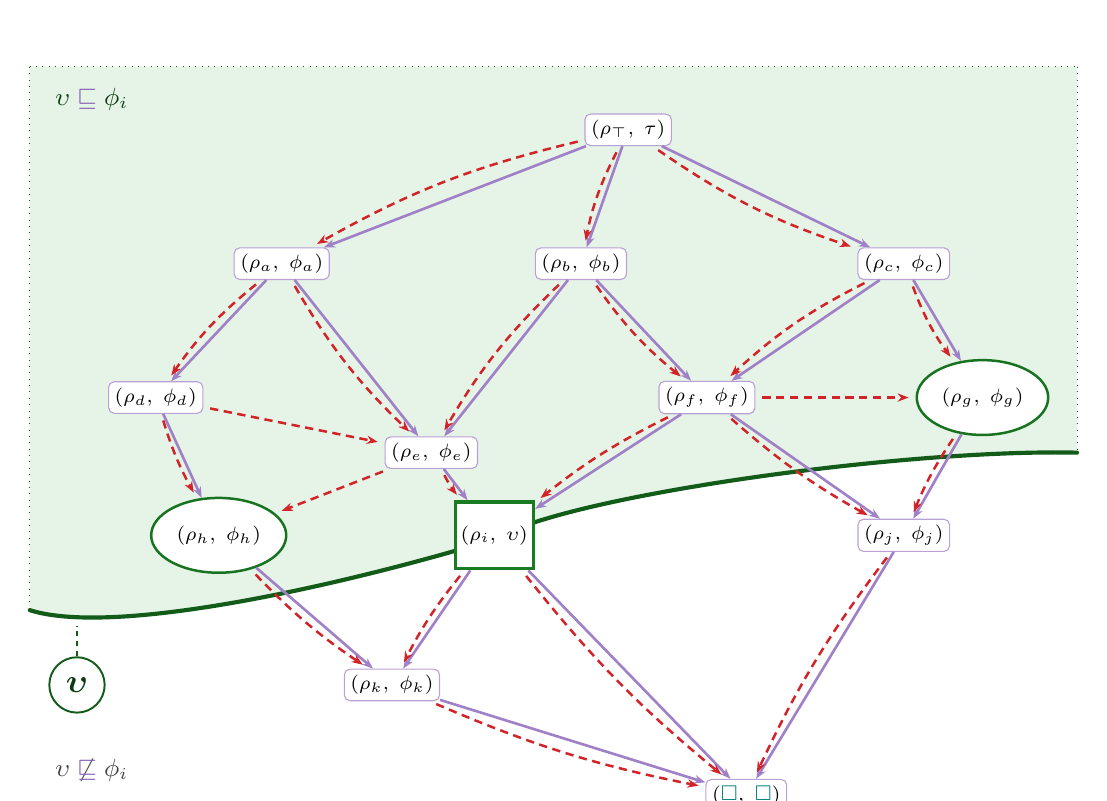
\begin{tikzpicture}[
    >={Stealth[length=4pt,width=3pt]},
    prognode/.style={draw=latticecolor!55, fill=white, rounded corners=2pt,
                     inner sep=2.2pt, font=\scriptsize},
    minnode/.style={draw=OliveGreen!70!black, fill=white, line width=0.9pt,
                    ellipse, minimum height=0.95cm,
                    inner xsep=2pt, inner ysep=2pt, font=\scriptsize},
    exactnode/.style={draw=OliveGreen!75!black, fill=white, line width=1.2pt,
                      rectangle, minimum width=0.85cm, minimum height=0.85cm,
                      inner sep=2pt, font=\scriptsize},
    progarrow/.style={->, latticecolor!75, line width=0.95pt},
    synarrow/.style={->, BrickRed, line width=0.9pt, dashed,
                     dash pattern=on 3pt off 2pt,
                     shorten >=2.5pt, shorten <=2.5pt}
]
\node[prognode]  (T)   at ( 0.0, 8.6) {$(\rho_\top,\;\tau)$};
\node[prognode]  (A)   at (-4.4, 6.9) {$(\rho_a,\;\phi_a)$};
\node[prognode]  (B)   at (-0.6, 6.9) {$(\rho_b,\;\phi_b)$};
\node[prognode]  (C)   at ( 3.5, 6.9) {$(\rho_c,\;\phi_c)$};
\node[prognode]  (D)   at (-6.0, 5.2) {$(\rho_d,\;\phi_d)$};
\node[prognode]  (E)   at (-2.5, 4.5) {$(\rho_e,\;\phi_e)$};
\node[prognode]  (F)   at ( 1.0, 5.2) {$(\rho_f,\;\phi_f)$};
\node[minnode]   (G)   at ( 4.5, 5.2) {$(\rho_g,\;\phi_g)$};
\node[minnode]   (H)   at (-5.2, 3.45) {$(\rho_h,\;\phi_h)$};
\node[exactnode] (I)   at (-1.7, 3.45) {$(\rho_i,\;\upsilon)$};
\node[prognode]  (J)   at ( 3.5, 3.45) {$(\rho_j,\;\phi_j)$};
\node[prognode]  (K)   at (-3.0, 1.55) {$(\rho_k,\;\phi_k)$};
\node[prognode]  (Bot) at ( 1.5, 0.15) {$(\gap,\;\gap)$};

\begin{scope}[on background layer]
  \fill[OliveGreen!12]
    (-7.6, 9.4) -- (-7.6, 2.50)
    .. controls (-6.5, 2.15) and (-3.5, 2.85) .. (-1.70, 3.40)
    .. controls (-0.8, 3.95) and ( 3.5, 4.55) .. ( 5.7, 4.50)
    -- (5.7, 9.4) -- cycle;
  \draw[OliveGreen!55!black, line width=1.5pt, line cap=round]
    (-7.6, 2.50)
    .. controls (-6.5, 2.15) and (-3.5, 2.85) .. (-1.70, 3.40)
    .. controls (-0.8, 3.95) and ( 3.5, 4.55) .. ( 5.7, 4.50);
  \draw[OliveGreen!50!black, line width=0.3pt, dotted]
    (-7.6, 9.4) -- (5.7, 9.4)
    (-7.6, 9.4) -- (-7.6, 2.50)
    ( 5.7, 9.4) -- ( 5.7, 4.50);
\end{scope}

\draw[progarrow] (T) -- (A);
\draw[progarrow] (T) -- (B);
\draw[progarrow] (T) -- (C);
\draw[progarrow] (A) -- (D);
\draw[progarrow] (A) -- (E);
\draw[progarrow] (B) -- (E);
\draw[progarrow] (B) -- (F);
\draw[progarrow] (C) -- (F);
\draw[progarrow] (C) -- (G);
\draw[progarrow] (D) -- (H);
\draw[progarrow] (E) -- (I);
\draw[progarrow] (F) -- (I);
\draw[progarrow] (F) -- (J);
\draw[progarrow] (G) -- (J);
\draw[progarrow] (H) -- (K);
\draw[progarrow] (I) -- (K);
\draw[progarrow] (I) -- (Bot);
\draw[progarrow] (J) -- (Bot);
\draw[progarrow] (K) -- (Bot);

\draw[synarrow] (T) to[bend right=8]  (A);
\draw[synarrow] (T) to[bend right=8]  (B);
\draw[synarrow] (T) to[bend right=8]  (C);
\draw[synarrow] (A) to[bend right=8]  (D);
\draw[synarrow] (A) to[bend right=8]  (E);
\draw[synarrow] (B) to[bend right=8]  (E);
\draw[synarrow] (B) to[bend right=8]  (F);
\draw[synarrow] (C) to[bend right=8]  (F);
\draw[synarrow] (C) to[bend right=8]  (G);
\draw[synarrow] (D) to[bend right=6]  (H);
\draw[synarrow] (E) to[bend right=6]  (I);
\draw[synarrow] (F) to[bend right=6]  (I);
\draw[synarrow] (F) to[bend right=6]  (J);
\draw[synarrow] (G) to[bend right=6]  (J);
\draw[synarrow] (H) to[bend right=6]  (K);
\draw[synarrow] (I) to[bend right=6]  (K);
\draw[synarrow] (I) to[bend right=6]  (Bot);
\draw[synarrow] (J) to[bend right=6]  (Bot);
\draw[synarrow] (K) to[bend right=6]  (Bot);

\draw[synarrow] (D) -- (E);
\draw[synarrow] (F) -- (G);
\draw[synarrow] (E) -- (H);

\node[exactnode] at (I) {$(\rho_i,\;\upsilon)$};

\node[circle, fill=white, draw=OliveGreen!55!black, line width=0.7pt,
      inner sep=1pt, minimum size=20pt,
      text=OliveGreen!35!black]
  at (-7.0, 1.55) (vlabel) {\large $\boldsymbol{\upsilon}$};
\draw[OliveGreen!55!black, line width=0.6pt, dashed,
      dash pattern=on 2pt off 1.6pt]
  (vlabel.north) -- (-7.0, 2.30);

\node[anchor=north west, font=\small\bfseries, OliveGreen!35!black]
  at (-7.4, 9.25) {$\upsilon \sqsubseteq \phi_i$};
\node[anchor=south west, font=\small\bfseries, gray!50!black]
  at (-7.4, 0.20) {$\upsilon \not\sqsubseteq \phi_i$};

\end{tikzpicture}
\caption{An example Hasse diagram of $\lfloor \rho_\top \rfloor$ overlayed with type precision relations (mostly induced by graduality). {\color{latticecolor}Purple}: program precision $\sqsubset$. {\color{BrickRed}Red}: type precision $\sqsubseteq$. {\color{OliveGreen!60!black}Ellipses}: minimal synthesis slices. {\color{OliveGreen!60!black}Square}: an exact minimal slice}
\label{fig:syn-slice-existence}
\end{figure}

Refining a query $\upsilon$ to a smaller $\upsilon' \sqsubseteq \upsilon$ descends further in the lattice, finding minima which are less precise, but consistent with, the previous slice for $\upsilon$.
\begin{theorem}[\po Monotonicity of minimal slices]\mechbox{minMono}\label{thm:mono}
If $\upsilon_1 \sqsubseteq \upsilon_2$ in $\lfloor\tau\rfloor$ and $m_2 : \minsynslice{D}{\upsilon_2}$, then there exists $m_1 : \minsynslice{D}{\upsilon_1}$ with $m_1.\rho \sqsubseteq m_2.\rho$.
\end{theorem}

\subsection{\yo Sub-slices}
\label{sec:sub-slices}
\mechfile{Slicing/Synthesis/\\FixedAssmsCalc}

In practice, a user may not arrive at a query atomically. One might look at a synthesised type, then refine the query to explore one component of it, then into a sub-component. For this use case we get successive queries forming a descending chain $\upsilon \sqsupseteq \upsilon' \sqsupseteq \upsilon'' \sqsupseteq \cdots$. Due to monotonicity, this chain can be associated with a chain of program slices $\rho \sqsupseteq \rho' \sqsubseteq \cdots$.

\paragraph{Example.} Refining $\upsilon = \mathbf{*}\Rightarrow\mathbf{*}$ to $\upsilon' = \mathbf{*}\Rightarrow\gap$ on $e = \mathbf{if}\;\mathbf{true}\;\mathbf{then}\;x\;\mathbf{else}\;y$:
\begin{center}
\fullslice{x : \sli{\mathbf{*} \Rightarrow \mathbf{*}}}{\sli{\mathbf{if}}\;\mathbf{true}\;\sli{\mathbf{then}\;x\;\mathbf{else}}\;\gap}
\quad$\xrightarrow{\upsilon' \sqsubseteq \upsilon}$\quad
\fullslice{x : \sli{\mathbf{*} \Rightarrow}\,\mathbf{*}}{\sli{\mathbf{if}}\;\mathbf{true}\;\sli{\mathbf{then}\;x\;\mathbf{else}}\;\gap}
\end{center}

\paragraph{Branch hopping.} This descending chain of program slices is useful because it intuitively aligns with the users thinking of \textit{refining} and existing slice, and retrieving a refined program consistent with the last query. Picking random minimal slices will not necessarily form such a chain, giving rise to `branch hopping' where highlighted regions switch between branches when refining the query, which is undesirable from a UX perspective. For example, refining $\upsilon = \mathbf{*}\Rightarrow\mathbf{*}$ to $\upsilon' = \gap\Rightarrow\mathbf{*}$:
\begin{center}
\fullslice{x : \sli{\mathbf{*} \Rightarrow \mathbf{*}}}{\sli{\mathbf{if}}\;\mathbf{true}\;\sli{\mathbf{then}\;x\;\mathbf{else}}\;\gap}
\quad$\xrightarrow{\upsilon' \sqsubseteq \upsilon}$\quad
\fullslice{y : \mathbf{*}\,\sli{\Rightarrow \mathbf{*}}}{\sli{\mathbf{if}}\;\mathbf{true}\;\sli{\mathbf{then}}\;\gap\;\sli{\mathbf{else}\;y}}
\end{center}

\subsection{\yo Decompositions}
\label{sec:decompositions}
\mechfile{Slicing/Synthesis/\\Decompositions}

Each compound typing rule comes with a \textit{slice combinator}: an operation that builds a synthesis slice from slices of the typing rule's premises, joining their shared assumptions. All minimal slices of compound terms can be expressed as minimal slices of the sub-terms combined with these combinators. This suggests the existence of a compositional rule constructing minimal slices from minimal slices of the sub-terms following the structure of typing derivations.

\begin{majortheorembox}
\mechbox{min-*-\\decomposability}%
\begin{theorem}[\yo Decompositions]\label{thm:decomp-master}
For each compound type rule $R$ with slice combinator $\oplus_R$, every minimal slice of an $R$-derivation factors as $\oplus_R(m_1,\ldots,m_n)$ for minimal sub-slices $m_i$ of the typing rule's subderivations at sub-queries determined by the rule.
\end{theorem}
\end{majortheorembox}
\mastercases

I give the two of the cases: the product rule and the let binding rule. The remaining cases are similar.

\subsubsection{\yo Products}
\label{sec:case-pair}

Given slices $s_1 : \synslice{D_1}{\upsilon_1}$ and $s_2 : \synslice{D_2}{\upsilon_2}$ for the two components of a pair $D = \synr{Pair}\,D_1\,D_2$, we form their product slice $s_1 \pairsyn s_2 : \synslice{D}{\upsilon_1 \times \upsilon_2}$ by joining the two assumption slices ($\gamma^{\sqcup} = \gamma_1 \sqcup \gamma_2$), and pairing the slices $(s_1.\varsigma, s_2.\varsigma)$, which synthesise (possibly more precise)\footnote{Due to $\gamma^{\sqcup}$ being larger than $\gamma_1$ and $\gamma_2$} types $\phi_1' \times \phi_2' \sqsupseteq s_1.\phi \times s_2.\phi \sqsupseteq \upsilon_1 \times \upsilon_2$. For this combinator, we get the following decomposition theorem:

\begin{thmcase}[\yo Case: Products]\mechbox{min-prod-\\decomposability}\label{thm:min-prod-decomp}
Let $m : \minsynslice{\synr{Pair}\,D_1\,D_2}{\upsilon_1 \times \upsilon_2}$. Then there exist minimal $m_1 : \minsynslice{D_1}{\upsilon_1}$ and $m_2 : \minsynslice{D_2}{\upsilon_2}$ with $m = m_1 \pairsyn m_2$.
\end{thmcase}

\paragraph{\yo Converse Failure}
\label{sec:ce-prod-not-closed-min}

However, the converse is not true:

\begin{counterexamplebox}
\mechbox{\textnormal{\textbf{¬}}\&syn-preserves-\\minimality}%
\begin{counterexample}[\yo Paired minimal slices are not necessarily minimal]\label{lem:prod-not-minimal}

Consider two minimal slices, both on query $* \Rightarrow *$:
\begin{center}
\fullslice{x : \sli{\mathbf{*} \Rightarrow}\, \mathbf{*},\; y : \mathbf{*}\, \sli{\Rightarrow \mathbf{*}}}{\sli{\mathbf{if}}\;\mathbf{true}\;\sli{\mathbf{then}\;x\;\mathbf{else}\;y}}
\quad \text{and}\quad
\fullslice{x : \sli{\mathbf{*} \Rightarrow \mathbf{*}}}{\sli{x}}
\end{center}
Note that left slice is minimal due to the assumption slice, omitting either $x$ or $y$ would no longer synthesise $* \Rightarrow *$. However, the pair combinator, which pairs the expression slices and joins the assumption slices, produces:
\begin{center}
\fullslice{x : \sli{\mathbf{*} \Rightarrow \mathbf{*}},\; y : \mathbf{*}\, \sli{\Rightarrow \mathbf{*}}}{\sli{(\mathbf{if}}\;\mathbf{true}\;\sli{\mathbf{then}\;x\;\mathbf{else}\;\slr{y},\; x)}}
\end{center}
Which is \textit{not} minimal, the $y$ outlined in red can be removed while still synthesising $(* \Rightarrow *) \times (* \Rightarrow *)$ (the natural product of the queries of the components).
\end{counterexample}
\end{counterexamplebox}

Hence, we cannot simply recurse through the typing derivation to calculate a slice on $\upsilon_1 \times \upsilon_2$ from sub-slices of the components on $\upsilon_1$ and $\upsilon_2$ respectively. Section~\ref{sec:algorithms} solves this issue.

\subsubsection{\yo Let Bindings}
\label{sec:let-decomp}

A more subtle case is of let-bindings, which has difference assumptions for its two premises:
\[\inference[\synr{Let}]{
  \synthesis{e_1}{\tau_1}
  &
  \synthesis[\Delta;\,\Gamma, x:\tau_1]{e_2}{\tau_2}
}{\synthesis{\mathbf{let}\;x = e_1\;\mathbf{in}\;e_2}{\tau_2}}\]
A slice of a let-expression can be constructed from a slice $s_1$ of the definition and a slice $s_2$ of the body, constrained with a assumption consistency condition: the body's used assumptions for the bound variable $x$ must be \textit{at most as precise as} the type synthesised by the slice of the definition:
\[ s_2.\gamma(x) \mathbin{\sqsubseteq} s_1.\phi \]
Then, upon joining the assumptions for the two slices, we must remove the assumption on $x$ from the body (notated $\gamma_{\setminus x}$, as this is now provided by the definition: 
\[s_1 \texttt{def} s\_2 \triangleq (s_1.\gamma \sqcup s_2.\gamma_{\setminus x},\; \mathbf{let}\;x = s_1.\varsigma\;\mathbf{in}\;s_2.\varsigma)\]

\begin{thmcase}[Case: Bindings]\mechbox{min-def-\\decomposability}\label{thm:min-def-decomp}
Let $m : \minsynslice{\synr{Let}\,D_1\,D_2}{\upsilon}$. Then there exists $\phi_1 \in \lfloor\tau_1\rfloor$ and minimal slices $m_1 : \minsynslice{D_1}{\phi_1}$ and $m_2 : \minsynslice{D_2}{\upsilon}$ satisfying $m_2.\gamma(x) \sqsubseteq m_1.\phi$, with $m = m_1 \mathbin{\mathsf{def}} m_2$.
\end{thmcase}

\subsection{\yo Contribution Slices}
\label{sec:join-slices}
\mechfile{Slicing/Synthesis/\\Synthesis}

A natural way represent a minimal slice that retains \textit{all} information relevant to a query type query would be to \textit{join} all minimal slices for the slices, which is clearly unique. For this to make sense, closure of synthesis slices under joins is the crucial, joining two synthesis slices explaining $\upsilon$ should still explain $\upsilon$ fully.

This is a second instance where exact synthesis slices are too strong, we do \textit{not} get that joining two exact slices synthesises exactly the joined query: 

\begin{counterexamplebox}
\mechbox{\textnormal{\textbf{¬}$\OLDsqcup$}syn-closed}%
\begin{counterexample}[\yo Joins do not preserve exactness]\label{lem:exact-not-closed}
Consider $D : \synthesis[(x : \mathbf{*})]{x}{\mathbf{*}}$. For the query $\upsilon = \gap$, consider two exact (but not minimal) slices: $x : \gap \vdash x {\color{BrickRed}\Uparrow} \gap$ and $x : * \vdash \gap {\color{BrickRed}\Uparrow} \gap$.

However, their join synthesises $*$: $x : * \vdash x {\color{BrickRed}\Uparrow} *$, despite the join of the queries being $\gap$. This synthesis is not exact.
\end{counterexample}
\end{counterexamplebox}

Even if we restrict this the exact slices to be minimal:

\begin{counterexamplebox}
\mechbox{\textnormal{\textbf{¬}$\OLDsqcup$}syn-preserves-\\join}%
\begin{counterexample}[\yo Joins do not preserve exactness, even under minimality]\label{lem:join-not-tight}
Consider $D = \synthesis[x : * \Rightarrow *]{(x, x)}{(\mathbf{*} \Rightarrow \mathbf{*}) \times (\mathbf{*} \Rightarrow \mathbf{*})}$.
Then for queries $\upsilon_1 = \gap \times (\gap \Rightarrow \mathbf{*})$ and $\upsilon_2 = (\mathbf{*} \Rightarrow \gap) \times \gap$, we get minimal slices $(x : \gap \Rightarrow *,\ (\gap, x))$ and $(x : * \Rightarrow \gap),\ (x, \gap)$ respectively.

Joining these minimal slices gives the original derivation $D$, which synthesises $(* \Rightarrow *) \times (* \Rightarrow *) \sqsupset (* \Rightarrow \gap) \times (\gap \Rightarrow *) = \upsilon_1 \times \upsilon_2$.
\end{counterexample}
\end{counterexamplebox}

However, the weaker validity condition for regular synthesis slices $\upsilon \sqsubseteq \phi$, does allow for join closure.

\begin{majortheorembox}
\mechbox{\_$\OLDsqcup$syn\_}%
\begin{theorem}[\yo Closure of Synthesis Slices under Join]\label{thm:join-syn}
For $s_1 : \synslice{D}{\upsilon_1}$ and $s_2 : \synslice{D}{\upsilon_2}$, then $s_1 \joinsyn s_2 : \synslice{D}{\upsilon_1 \sqcup \upsilon_2}$ with program slice $\rho^{\sqcup} = \rho_1 \sqcup \rho_2$.
\end{theorem}
\end{majortheorembox}

\begin{figure}[t]
\centering
\begin{tikzcd}[column sep=large, row sep=large]
\rho_1 \arrow[r, "\sqsubseteq"] \arrow[d, "{\color{BrickRed}\Uparrow}"'] & {\color{induced} \rho^{\sqcup}} \arrow[d, "{\color{BrickRed}\Uparrow}"] & \rho_2 \arrow[l, "\sqsupseteq"'] \arrow[d, "{\color{BrickRed}\Uparrow}"] \\
\phi_1 & {\color{induced} \phi'} & \phi_2 \\
\upsilon_1 \arrow[u, "\sqsubseteq" {sloped}] \arrow[r, "\sqsubseteq"] & {\color{induced} \upsilon_1 \sqcup \upsilon_2} \arrow[u, induced, "\sqsubseteq"' {sloped}, dashed] & \upsilon_2 \arrow[u, "\sqsubseteq"' {sloped}] \arrow[l, "\sqsupseteq"']
\end{tikzcd}
\caption{Theorem~\ref{thm:join-syn}.}
\label{fig:join-validity}
\end{figure}

%%% Local Variables:
%%% mode: LaTeX
%%% TeX-master: "PolymorphicTypeSlicing"
%%% End:

\section{Analysis Slices}
\label{sec:analysis}

\sectionlegend

\providecommand{\anaslice}[2]{\mathit{AnaSlice}\;#1 \mathbin{\blacktriangleleft} #2}
\providecommand{\minanaslice}[2]{\mathit{MinAnaSlice}\;#1 \mathbin{\blacktriangleleft} #2}
\providecommand{\anaposslice}[2]{\mathit{AnaPosSlice}\;#1 \mathbin{\blacktriangleleft} #2}
\providecommand{\minanaposslice}[2]{\mathit{MinAnaPosSlice}\;#1 \mathbin{\blacktriangleleft} #2}

\noindent Analysis slices are the construction for sub-terms that are \textit{analysed} against an expected type rather than synthesising one. The principal difference from synthesis slices is the object being sliced: where a synthesis slice sliced a derivation $D : \synthesis{e}{\tau}$, an analysis slice slices a \textit{context classification} $\ctxclass{\C}{d}{\Delta';\,\Gamma'}{m}$ (Appendix~\ref{app:ctx-classification}) around the selected term. The expression slice $\varsigma$ is replaced by a context slice $\kappa \in \lfloor\C\rfloor$; everything else (minimality, existence, monotonicity) proceeds analogously to Section~\ref{sec:synthesis}, with the same non-exactness phenomena recurring for the outer-type witness.

\subsection{\yo Analysis Slices}
\label{sec:ana-slice-def}
\mechfile{Slicing/Analysis/\\Analysis}

Analysis slices concern the classifications with focus mode $m = {\color{BlueViolet}\Leftarrow}\tau$. A query $\upsilon \in \lfloor\tau\rfloor$ specifies the part of $\tau$ that we wish to explain. The outer derivation mode $d$ splits the construction in two; the second is a strengthening of the first, needed because some classification rules cross from synthesis-position outer to analysis-position inner (notably $s\circ_2$, the application focused on its argument).

\begin{definition}[\yo Analysis slice]
\label{def:ana-slice}
An \textit{analysis slice} of $\mathit{Cls} : \ctxclass{\C}{{\color{BrickRed}\Uparrow}\,\tau_p}{\Delta';\,\Gamma'}{{\color{BlueViolet}\Leftarrow}\,\tau}$ on $\upsilon \in \lfloor\tau\rfloor$, written $\anaslice{\mathit{Cls}}{\upsilon}$, is a four-tuple
\[ (\kappa,\,\gamma) \mathbin{{\color{BlueViolet}\Downarrow}} \psi \mathbin{\sqsupseteq} \upsilon \mathbin{\in} \mathit{cls}' \]
with $(\kappa, \gamma) \in \lfloor\C, \Gamma\rfloor$, an outer-type witness $\psi \in \lfloor\tau_p\rfloor$, and $\mathit{cls}' : \ctxclass[\Delta;\,\gamma]{\kappa}{{\color{BrickRed}\Uparrow}\,\psi}{\Delta'';\,\Gamma''}{{\color{BlueViolet}\Leftarrow}\,\upsilon}$.
\end{definition}

\begin{definition}[\yo Analysis position slice]
\label{def:ana-pos-slice}
An \textit{analysis position slice} of $\mathit{Cls} : \ctxclass{\C}{{\color{BlueViolet}\Downarrow}\,\tau_p}{\Delta';\,\Gamma'}{{\color{BlueViolet}\Leftarrow}\,\tau}$ on $\upsilon \in \lfloor\tau\rfloor$, written $\anaposslice{\mathit{Cls}}{\upsilon}$, is a four-tuple
\[ (\kappa,\,\gamma) \mathbin{{\color{BlueViolet}\Downarrow}} \upsilon \mathbin{\Downarrow} \upsilon_{\mathrm{outer}} \mathbin{\in} \mathit{cls}' \]
with $(\kappa, \gamma) \in \lfloor\C, \Gamma\rfloor$, an outer-type witness $\upsilon_{\mathrm{outer}} \in \lfloor\tau_p\rfloor$, and $\mathit{cls}' : \ctxclass[\Delta;\,\gamma]{\kappa}{{\color{BlueViolet}\Downarrow}\,\upsilon_{\mathrm{outer}}}{\Delta'';\,\Gamma''}{{\color{BlueViolet}\Leftarrow}\,\upsilon}$.
\end{definition}

The two notions are mutually recursive: $s\circ_2$ embeds an analysis-position sub-classification inside a synthesis-position outer, while $aSub$ and $adef_1$ embed a synthesis-position sub-classification inside an analysis-position outer. The outer-type witnesses $\psi$ and $\upsilon_{\mathrm{outer}}$ play the role of $\phi$ in a synthesis slice, and exhibit the same non-existence and join-non-exactness phenomena (Counterexamples~\ref{lem:exact-not-exist}, \ref{lem:exact-not-closed}, \ref{lem:join-not-tight}); the weaker $\sqsupseteq$ validity condition is adopted in both definitions for the same reasons.

\begin{figure}[t]
\centering
\begin{tikzcd}[column sep=large, row sep=large]
& (\kappa,\gamma) \arrow[r, "\sqsubseteq" {sloped}] \arrow[d, "{\color{BlueViolet}\Downarrow}"'] & (\C,\Gamma) \arrow[d, "{\color{BlueViolet}\Downarrow}"] \\
\upsilon \arrow[r, "\sqsubseteq" {sloped}] & \psi \arrow[r, induced, "\sqsubseteq" {sloped}, "\text{(by graduality)}"', dashed] & \tau_p
\end{tikzcd}
\caption{Diagram of an analysis slice; $\upsilon \sqsubseteq \psi$ is the validity witness on the outer-type witness side ($\upsilon_{\mathrm{outer}}$ for an analysis position slice).}
\label{fig:ana-fundamental-triangle}
\end{figure}

\subsection{\yo Minimality}
\label{sec:ana-minimality}
\mechfile{Slicing/Analysis/\\Analysis}

$\minanaslice{\mathit{Cls}}{\upsilon}$ and $\minanaposslice{\mathit{Cls}}{\upsilon}$ are defined analogously to Definition~\ref{def:isminimal}, minimising over the context slice $(\kappa, \gamma)$. The outer-type witness is determined up to the slice lattice by the lifted classification and is not minimised over independently.

Minimal analysis slices need not be unique, but this non-determinism is wholly inherited from synthesis: the expected types against which sub-terms are analysed are themselves derived from types synthesised elsewhere in the program, and those synthesis slices can have multiple incomparable minima (Counterexample~\ref{lem:min-not-unique}). Analysis slicing introduces no new sources of non-determinism beyond this.

\subsection{\po Existence}
\label{sec:ana-min-exists}
\mechfile{Slicing/Analysis/\\Analysis}

\begin{majortheorembox}
\mechbox{minExists/\\minExistsPos}%
\begin{theorem}[\po Existence of minimal analysis slices]\label{thm:ana-min-exists}
For every $s : \anaslice{\mathit{Cls}}{\upsilon}$, there exists $m : \minanaslice{\mathit{Cls}}{\upsilon}$ with $m \sqsubseteq s$; and analogously for $\mathit{AnaPosSlice}$.
\end{theorem}
\end{majortheorembox}

\begin{proof}
The slice lattice $\lfloor\C, \Gamma\rfloor$ is finite, so $\{(\kappa', \gamma') \sqsubseteq (\kappa, \gamma) \mid (\kappa', \gamma')\,\text{is a slice}\}$ is finite. Enumerate it and descend; the chain terminates at a minimal element.
\end{proof}

\subsection{\po Monotonicity}
\label{sec:ana-monotonicity}
\mechfile{Slicing/Analysis/\\Analysis}

\begin{theorem}[\po Monotonicity of minimal analysis slices]\mechbox{mono/monoPos}\label{thm:ana-mono}
If $\upsilon_1 \sqsubseteq \upsilon_2$ in $\lfloor\tau\rfloor$ and $m_2 : \minanaslice{\mathit{Cls}}{\upsilon_2}$, then there exists $m_1 : \minanaslice{\mathit{Cls}}{\upsilon_1}$ with $m_1.\kappa \sqsubseteq m_2.\kappa$ and $m_1.\gamma \sqsubseteq m_2.\gamma$; analogously for $\mathit{AnaPosSlice}$.
\end{theorem}

\clearpage

%%% Local Variables:
%%% mode: LaTeX
%%% TeX-master: "PolymorphicTypeSlicing"
%%% End:

\section{Error Marking \& Type Error Debugging}
\label{sec:marking}
\mechfile{Semantics/Marking/}

\sectionlegend

This chapter associates the tools of this formalism with the proposed UX for debugging type errors (\cref{sec:ui}). It demonstrates that we can not only use this calculus to ``explain types'' in well-typed programs, but also effectively ``explain type errors'' in ill-typed programs.

This builds upon the theory of type error marking for bidirectional systems with holes of Zhao et al.~\cite{Marking2024}, which I briefly recap and extend to the type slicing core calculus (\cref{sec:core-calculus}) in the next subsection.
 
\subsection{\yo Error Marking}
\label{sec:marking-calculus}
\mechfile{Semantics/Marking/\\Judgment}

A marking algorithm is a pair of bidirectional judgements,
\[
  \synmark{e}{\chk e}{\tau}
  \qquad\text{and}\qquad
  \anamark{e}{\chk e}{\tau},
\]
reading ``under $\Delta;\Gamma$, the source expression $e$ \textit{marks
to} the marked expression $\chk e$, synthesising (resp.\ being analysed
against) type $\tau$''. The marked output $\chk e$ has the same
structure as $e$ but wraps each point of local type failure in a \emph{mark}. The marks, representing highlighting an entire erroneous term $e$, are tabulated in \cref{tab:mark-forms} alongside the corresponding typing rule failures. 

The core calculus studied gives rise to four classes of errors: \textit{type inconsistencies} when subsumption cannot be applied, \textit{shape errors} when rules expect a sub-term to join (match) a specific type shape, \textit{mode limitations} where syntax which cannot synthesise its type is expected to provide type information. And variable \textit{scoping errors}, which do not pertain to types, so cannot be debugged by type slicing.

\begin{table}[h]
\centering
\small
\begin{tabularx}{\linewidth}{lll : X}
\toprule
\textbf{Mark} & \textbf{Class} & \textbf{Failed Rule(s)} & \textbf{Error} \\
\midrule
$\markincon[e]{\tau'}{\tau}$ & type inconsistency & Subsumption & $e$ synthesises $\tau'$ inconsistent with analysis type $\tau$ \\
$\markarrow[e]$       & shape & Function Application & $e$ is in a function position, but is not a function \\
$\marksum[e]$         & shape & Case Expression & $e$ is a case scrutinee, but is not a sum type \\
$\markprod[e]$        & shape & Product Projection & $e$ is projected as a product, but is not a product \\
$\markforall[e]$      & shape & Typfun Application & $e$ is in a typfun positon, but is not a typfun \\
$\marklam[\lambda x.\,e]$ & mode limitation & Lambda Synthesis & Unannotated lambda in synthesis position \\
$\marklam[\lambda x.\,e]$ & mode limitation & Lambda Analysis  & Unannotated lambda analysed against a non-function type \\
$\markinj[\iota_i\,e]$    & mode limitation & Sum Injections   & Sum injections in synthesis position \\
$\markvar{k}$      & scope & Variables & Variable $k$ has no binding in scope \\
\bottomrule
\end{tabularx}
\caption{Error Mark Forms Classified}
\label{tab:mark-forms}
\end{table}

Importantly, marked terms can be type-checked by treating the marked terms as `non-empty' holes, synthesising $\gap$ (and recursively marking and type-checking the inner term).

The validity of this method is formalised by two theorems: \textit{totality} ensures marks account for every possible typing error, and \textit{erasure} ensures adding marks doesn't change the structure of the terms.

\begin{theorem}[\yo Totality of Marking]
\label{thm:mark-total}
\mechbox{Semantics/Marking/\\Metatheory}
For every expression $e$ and assumptions $\Delta;\Gamma$. There exists marked expression $\chk e$ and type $\tau$ such that
$\synmark{e}{\chk e}{\tau}$. And, for every type $\tau'$, there exists
$\chk e'$ such that $\anamark{e}{\chk e'}{\tau}$.
\end{theorem}

\begin{theorem}[\yo Erasure of Marking]
\label{thm:mark-erase}
\mechbox{Semantics/Marking/\\Metatheory}
If $\synmark{e}{\chk e}{\tau}$ then $\mathrm{erase}(\chk e) \equiv e$, and
likewise for analysis.
\end{theorem}

\paragraph{Mechanisation provenance.}
The Agda development is loosely based on the mechanisation accompanying
\textcite{Marking2024} --
\href{https://github.com/hazelgrove/error-localization-agda}{\texttt{hazelgrove/error-localization-agda}}
-- but the proofs are not direct ports. They were re-derived from
scratch against the core calculus of \cref{sec:core-calculus}, following the recipe proposed in the paper.

\subsection{\yo Marked Context Classification}
\label{sec:marking-classification}
\mechfile{Semantics/Marking/\\CtxMarking}

Context classification (\cref{sec:context-classification-section}) gives a
reading of where a one-hole context $C$ sits in a derivation.
This can be extended to marked context classification
$\mctxclass[\Delta;\Gamma]{C}{\chk C}{p}{\Delta';\Gamma'}{m}$ threads a
marked context $\chk C$ alongside $C$ (with context marks defined analogously to expressions), with one error rules per mark form in \cref{tab:mark-forms}.

For example, the type inconsistency mark can be inserted into context classification with the following rule:
\[
\inference[$maSub{\Uparrow}$]
  {\mctxclass[\Delta;\Gamma]{C}{\chk C}{{\color{BrickRed}\Uparrow}\;\tau'}{\Delta';\Gamma'}{m}
   & \neg(\tau \sim \tau')}
  {\mctxclass[\Delta;\Gamma]{C}{\markincon[\chk C]{\tau'}{\tau}}{{\color{BlueViolet}\Downarrow}\;\tau}{\Delta';\Gamma'}{m}}
\]
The marked context wraps the inner marked context $\chk C$ in an inconsistency mark when the analysed and synthesised types of the \textit{full plugged expression} differ: $\tau' \not\sim \tau$. The full rule set is collected in \cref{app:ctx-classification}.

\paragraph{\yo A Worked Decomposition}
\label{sec:marking-classification-insideout}

Take the expression:
\[
  \mathbf{let}\;p : * \times (* \Rightarrow *) = (\,*,\,\texttt{true}\,)\;\mathbf{in}\;p.
\]
The pair's right component synthesises $\texttt{Bool}$ but is
analysed against $* \Rightarrow *$ (from the annotation), so marking should produce:
\[
  \mathbf{let}\;p : * \times (* \Rightarrow *) = (\,*,\,\markincon[\texttt{true}]{\texttt{Bool}}{* \Rightarrow *}\,)\;\mathbf{in}\;p.
\]
Placing the focus on the marked term $\texttt{true}$ gives:
\[
  C \;=\; \mathbf{let}\;p : * \times (* \Rightarrow *) = (\,*,\,\cmark\,)\;\mathbf{in}\;p,
  \qquad
  e \;=\; \texttt{true}.
\]
The classification builds $\chk C$ from the inside out, first marking the focus with the type inconsistency:
\begin{center}
\small
\begin{tabular}{ll}
\toprule
\textbf{Step (rule)} & \textbf{$\chk C$ so far} \\
\midrule
$\mathsf{ms}\circ$              & $\cmark$ \\
$maSub\!\Uparrow$               & $\markincon[\cmark]{\texttt{Bool}}{* \Rightarrow *}$ \\
$\mathsf{ma}\&_2$               & $(\,*,\,\markincon[\cmark]{\texttt{Bool}}{* \Rightarrow *}\,)$ \\
$\mathsf{ma}\textsf{let}\ldots$ & $\mathbf{let}\;p : * \times (* \Rightarrow *) = (\,*,\,\markincon[\cmark]{\texttt{Bool}}{* \Rightarrow *}\,)\;\mathbf{in}\;p$ \\
\bottomrule
\end{tabular}
\end{center}
Plugging gives $\chk C[\texttt{true}]$:
\[
  \mathbf{let}\;p : * \times (* \Rightarrow *) = (\,*,\,\markincon[\texttt{true}]{\texttt{Bool}}{* \Rightarrow *}\,)\;\mathbf{in}\;p.
\]

Marked context classification is validated with a pair of theorems mirroring the unmarked
$\mathit{plug}$ totality and soundness theorems
(\cref{thm:plug-decomposition,thm:plug-composition}).

\begin{majortheorembox}
\mechbox{mplug-\\decompose}%
\begin{theorem}[\yo Marked Plug Decomposition -- Totality]\label{thm:mplug-decompose}
For any context $\C$, expression $e$, and outer derivation mode $d$:
\begin{itemize}
\item If\/ $\synmark{\C[e]}{\chk{e_\star}}{\tau}$, then there exist $\Delta'$, $\Gamma'$, $\chk\C$, $\chk e$, and $m$ such that $\mctxclass{\C}{\chk\C}{{\color{BrickRed}\Uparrow}\;\tau}{\Delta';\,\Gamma'}{m}$, $e$ marks to $\chk e$ at focus mode $m$, and $\chk{e_\star} = \chk\C[\chk e]$.
\item If\/ $\anamark{\C[e]}{\chk{e_\star}}{\tau}$, then there exist $\Delta'$, $\Gamma'$, $\chk\C$, $\chk e$, and $m$ such that $\mctxclass{\C}{\chk\C}{{\color{BlueViolet}\Downarrow}\;\tau}{\Delta';\,\Gamma'}{m}$, $e$ marks to $\chk e$ at focus mode $m$, and $\chk{e_\star} = \chk\C[\chk e]$.
\end{itemize}
Here ``$e$ marks to $\chk e$ at focus mode $m$'' means: if $m = {\color{BrickRed}\Rightarrow}\;\tau'$ then $\synmark[\Delta';\,\Gamma']{e}{\chk e}{\tau'}$; if $m = {\color{BlueViolet}\Leftarrow}\;\tau'$ then $\anamark[\Delta';\,\Gamma']{e}{\chk e}{\tau'}$.
\end{theorem}
\end{majortheorembox}

\begin{majortheorembox}
\mechbox{mplug-\\compose}%
\begin{theorem}[\yo Marked Plug Composition -- Soundness]\label{thm:mplug-compose}
For any context $\C$, marked context $\chk\C$, outer derivation mode $d$, and focus mode $m$: if\/ $\mctxclass{\C}{\chk\C}{d}{\Delta';\,\Gamma'}{m}$ and $e$ marks to $\chk e$ at focus mode $m$, then $\C[e]$ marks to $\chk\C[\chk e]$ at outer derivation mode $d$.
\end{theorem}
\end{majortheorembox}

\subsection{\no The Debugging Recipe by Example}
\label{sec:marking-recipes}

We may now relate the tools developed over the last 4 sections to explain type errors:
\begin{enumerate}
\item Place the focus (cursor) at some marked term. This splits the marked program into a marked context $\chk C$ and marked focus $\chk e$, with $\chk C[\chk e]$ recovering the program; a marked context classification at the focus is then derivable by totality (\cref{thm:mplug-decompose}).
\item Synthesis slice the internal type information, the term at the \emph{focus}, $\chk e$, if the focus mode $m$ is in synthesis (${\color{BrickRed}\Uparrow}\;\tau$).
\item Analysis slice the external type information, the \emph{context classification} itself, if the focus mode $m$ is in analysis (${\color{BlueViolet}\Downarrow}\;\tau$).
\item Pick queries to explore the error. For type-inconsistency marks both the synthesis and analysis slices exist (context classifications for both steps 2 and 3 exist), and you can query \textit{only} the inconsistent parts. For shape errors, query just the outermost shape of the synthesised type; mode-limitation errors are analogous on the analysis side.
\end{enumerate}

I give some worked examples, with the following notation:
\begin{itemize}
\item The marked term itself is wrapped in a \markbox{\text{red dashed box}}.
\item The synthesis slice of the focus is highlighted in \sli{\text{blue}}.
\item The analysis slice of the surrounding context is highlighted in \sli[OliveGreen]{\text{green}}. With purely structural parts which don't contribute to the type (i.e. bindings) in a lighter shade.\footnote{This idea of 'purely' structural parts is not formalised here, but is easy to implement in practice.}
\end{itemize}

\subsubsection{Type inconsistency: \texorpdfstring{$\markincon{\tau'}{\tau}$}{type inconsistency}}
\label{sec:marking-recipes-incon}

Consider the program
\[
  \mathbf{let}\;p : * \Rightarrow * = (\texttt{true},\,\texttt{false})\;\mathbf{in}\;p.
\]
The RHS $(\texttt{true},\,\texttt{false})$ synthesises $\texttt{Bool} \times \texttt{Bool}$ but is analysed against $* \Rightarrow *$ --- inconsistent head constructors. Marking inserts
$\markincon{\texttt{Bool} \times \texttt{Bool}}{* \Rightarrow *}$
around the RHS:
\[
  \mathbf{let}\;p : * \Rightarrow * = \markbox{\markincon[(\texttt{true},\,\texttt{false})]{\texttt{Bool} \times \texttt{Bool}}{* \Rightarrow *}}\;\mathbf{in}\;p.
\]

\paragraph{Decomposition.}
The (context, focus) pair the marking factors into is
\[
  C \;=\; \mathbf{let}\;p : * \Rightarrow * = \cmark\;\mathbf{in}\;p,
  \qquad
  e \;=\; (\texttt{true},\,\texttt{false}),
\]
with the focus at ${\color{BlueViolet}\Downarrow}\,(* \Rightarrow *)$. The two
debugging queries run on the two sides of this split.

\paragraph{Synthesis side (blue, on the focus $e$).}
$\mathit{MinSynSlice}$ at the minimal type-slice $\upsilon \sqsubseteq \texttt{Bool} \times \texttt{Bool}$ that still witnesses $\upsilon \not\sim (* \Rightarrow *)$:
\[
  e \;\rightsquigarrow\; (\,\texttt{true}\,\sli{,}\,\texttt{false}\,)
  \qquad\text{with}\qquad
  \upsilon = \gap\,\sli{\times}\,\gap.
\]

\paragraph{Analysis side (green, on the context $C$).}
$\mathit{MinAnaSlice}$ at the minimal $\psi \sqsubseteq * \Rightarrow *$ that still witnesses $(* \times *) \not\sim \psi$:
\[
  C \;\rightsquigarrow\;
  \slist{\mathbf{let}}\;p\,\slist{:}\,*\,\sli[OliveGreen]{\Rightarrow}\,*\,\slist{=}\,\cmark\,\slist{\mathbf{in}}\;p
  \qquad\text{with}\qquad
  \psi = \gap\,\sli[OliveGreen]{\Rightarrow}\,\gap.
\]

\paragraph{Full view.}
\queryblock{\texttt{Bool}\sli{\times}\texttt{Bool}\;\;(\equiv\;\gap \times \gap)}{\sli[OliveGreen]{\texttt{*}\Rightarrow\texttt{*}}\;\;(\equiv\;\gap \Rightarrow \gap)}
\[
  \slist{\mathbf{let}}\;p\,\slist{:}\,*\,\sli[OliveGreen]{\Rightarrow}\,*\,\slist{=}\,
  \markbox{\markincon[(\,\texttt{true}\,\sli{,}\,\texttt{false}\,)]{\texttt{Bool} \times \texttt{Bool}}{* \Rightarrow *}}\,
  \slist{\mathbf{in}}\;p.
\]
The slices pick out exactly what each side contributes to the failure.

The recipe approach does not arbitrarily blame either the synthesising term or the analysing context for the error. A user who does want to trust the surrounding context (typically, annotations) as is often done in conventional type error highlighting can simply restrict the queries to include only the synthesis-side.

\subsubsection{Shape mismatches: $\markarrow$, $\marksum$, $\markprod$, $\markforall$}
\label{sec:marking-recipes-shape}

The shape-mismatch marks ($\markarrow$, $\marksum$, $\markprod$, $\markforall$) all share the same simple recipe: the syntactic position of the focus requires a type kind, but the focus's synthesised type does not match this.

A representative example is $e = \texttt{true}\,(\,*\,)$: the function position synthesises $\texttt{Bool}$, which is a function, i.e. does not join with $\gap \Rightarrow \gap$:
\queryblock{\sli{\texttt{Bool}}}{\text{---}}
\[
  \markbox{\markarrow[\sli{\texttt{true}}]}\,(\,*\,).
\]
$\marksum$ ($\mathbf{case}\;*\;\mathbf{of}\;\ldots$), $\markprod$ ($\pi_1\,\texttt{true}$), and $\markforall$ are analogous.

\subsubsection{Unannotated Lambda against Non-Arrow: \texorpdfstring{$\marklam$}{bare-lambda}}
\label{sec:marking-recipes-lam}

Unannotated lambdas $\lambda y.\,e$ have no synthesis rule, type must be
by the surrounding context. Consequentially it has
no synthesis type, so type inconsistencies are not marked via subsumption, but instead by a mode limitation mark. In this situation all the relevant type information is derived from the surrounding context, so we use analysis slices.

Consider the program:
\[
  \mathbf{let}\;b : \texttt{Bool} = \lambda y.\,y\;\mathbf{in}\;b.
\]
The RHS $\lambda y.\,y$ is a bare lambda analysed against
$\texttt{Bool}$. Take the $\mathit{MinAnaSlice}$ on the enclosing context witnesses the context enforcing a non-function type (\texttt{Bool}):
\queryblock{\text{---}}{\sli[OliveGreen]{\texttt{Bool}}}
\[
  \slist{\mathbf{let}}\;b\,\slist{:}\,\sli[OliveGreen]{\texttt{Bool}}\,\slist{=}\,
  \markbox{\marklam[\lambda y.\,y]}\,\slist{\mathbf{in}}\;b.
\]
The injection mark $\markinj$ follows the same pattern.

\subsubsection{Unbound variable: \texorpdfstring{$\markvar{k}$}{unbound}}
\label{sec:marking-recipes-unbound}

The free-variable mark records a \emph{scope} failure: there are no types involved.

\subsection{\no Assumption Slices}
\label{sec:marking-assumption-slices}

The involved synthesis slices also slice their required assumptions. In a closed program with the context-classification focus placed,
every free variable in the focus's available assumptions $\Gamma'$ has a unique binder. At each binder the type information comes from synthesis of a subterm, by type annotation, or for unannotated functions comes from the context. We can query these to find minimal sub-terms or contexts which provide the smaller assumption required by the assumption slice.

\begin{center}
\small
\begin{tabular}{lll}
\toprule
\textbf{Binder} & \textbf{Query kind} & \textbf{Slice runs on} \\
\midrule
$\mathbf{let}\;x = e\;\mathbf{in}\;\ldots$            & synthesis slice & the definition $e$ \\
$\mathbf{case}\;s\;\mathbf{of}\;x.\,e \mid y.\,e'$    & synthesis slice & the scrutinee $s$ \\
$\lambda x{:}\tau.\,e$                                & type slice & the annotation $\tau$ \\
$\lambda x.\,e$                                       & analysis slice & the surrounding context \\
\bottomrule
\end{tabular}
\end{center}

To get a slice for the full program, transitively query each assumption in the assumption slices. \textit{However}, such a transitive slice will not necessarily be minimal, as the term slices corresponding to assumptions may not be exact, so the actual assumptions provided may be larger than the assumption slice. In theory, this could be tracked using the assumptions threaded through the context classification construct but I leave this to further work.

\paragraph{Module boundaries.}
Not all programs are closed. For a program importing a module without source, the assumptions slice genuinely describes a minimal module import required to produce a type. This extends to specifying exactly which parts of imported compound module values are required (e.g. which parts of a product are needed), which would be relevant for a system that used gradual types to express partial imports of compound module values.

%%% Local Variables:
%%% mode: LaTeX
%%% TeX-master: "PolymorphicTypeSlicing"
%%% End:

\section{Optimising Type Slice Calculation}
\label{sec:algorithms}

\sectionlegend

\providecommand{\tmslice}[2]{\mathit{TermMin}\;#1 \mathbin{\blacktriangleleft} #2}
\providecommand{\mintmslice}[2]{\mathit{MinTermMin}\;#1 \mathbin{\blacktriangleleft} #2}
\providecommand{\tmcalc}[5]{#1 \mathbin{{\color{BrickRed}\blacktriangleleft}} #2 \;{\color{BrickRed}\rightsquigarrow}\; #3 \mathbin{{\color{BrickRed}\Uparrow}} #4 \,\dashv\, #5}
\providecommand{\tmrule}[7][\Delta;\,\Gamma]{%
  #1 \vdash #2 \mathbin{{\color{BrickRed}\Uparrow}} #3
  \mathbin{{\color{BrickRed}\blacktriangleleft}} #4
  \;{\color{BrickRed}\rightsquigarrow}\; #5
  \mathbin{{\color{BrickRed}\Uparrow}} #6
  \,\dashv\, #7%
}

\providecommand{\stkU}[2]{%
  \tikz[baseline=(N.base)]{%
    \node[inner sep=0pt, outer sep=0pt] (N) {\strut$#2$};%
    \foreach \col/\off in {#1}{%
      \draw[\col, line width=1.2pt, line cap=butt, overlay]
        ([xshift=-3pt,yshift=\off]N.south west) -- ([xshift=3pt,yshift=\off]N.south east);%
    }%
    \path ([yshift=-10pt]N.south west) ([yshift=-10pt]N.south east);%
  }%
}
\providecommand{\tokensp}{\mskip8mu}
\providecommand{\sABCD}[1]{\stkU{BrickRed/-1pt,NavyBlue/-3.4pt,OliveGreen/-5.8pt,Mulberry/-8.2pt}{#1}}
\providecommand{\sABC}[1]{\stkU{BrickRed/-1pt,NavyBlue/-3.4pt,OliveGreen/-5.8pt}{#1}}
\providecommand{\sABD}[1]{\stkU{BrickRed/-1pt,NavyBlue/-3.4pt,Mulberry/-8.2pt}{#1}}
\providecommand{\sAC}[1]{\stkU{BrickRed/-1pt,OliveGreen/-5.8pt}{#1}}
\providecommand{\sAD}[1]{\stkU{BrickRed/-1pt,Mulberry/-8.2pt}{#1}}
\providecommand{\sBC}[1]{\stkU{NavyBlue/-3.4pt,OliveGreen/-5.8pt}{#1}}
\providecommand{\sBD}[1]{\stkU{NavyBlue/-3.4pt,Mulberry/-8.2pt}{#1}}
\providecommand{\sC}[1]{\stkU{OliveGreen/-5.8pt}{#1}}
\providecommand{\sD}[1]{\stkU{Mulberry/-8.2pt}{#1}}
\providecommand{\sPone}[1]{\stkU{OliveGreen/-1pt}{#1}}
\providecommand{\sPtwo}[1]{\stkU{Mulberry/-3.4pt}{#1}}
\providecommand{\sPboth}[1]{\stkU{OliveGreen/-1pt,Mulberry/-3.4pt}{#1}}

\bigskip
\noindent The theory of Sections~\ref{sec:synthesis}--\ref{sec:analysis} establishes \textit{which} slices exist, and provide a brute-force algorithm. This section explores these structures further to improve the brute-force algorithm.

\subsection{\yo Products of Synthesis Slices}
\label{sec:product-revisited}
\mechfile{Slicing/Synthesis/\\FixedAssmsCalc}

The product counterexample of Section~\ref{sec:ce-prod-not-closed-min} is worth re-examining, which stated that not all pairs of minimal slices can be paired into a minimal product slice. Consider the following if statement:
\[ \Gamma = (x \mathbin{:} \mathbf{*} \Rightarrow \mathbf{*},\; y \mathbin{:} \mathbf{*} \Rightarrow \mathbf{*}), \qquad e = \mathbf{if}\;\mathbf{true}\;\mathbf{then}\;x\;\mathbf{else}\;y, \qquad \tau = \mathbf{*} \Rightarrow \mathbf{*}, \]
and ask for slices of $D : \synthesis{e}{\tau}$ at the full query $\upsilon = \mathbf{*} \Rightarrow \mathbf{*}$. There are \textit{four} incomparable minimal full slices, displayed together as underlines:

\begin{center}
\begin{tikzpicture}[baseline=(t.base), every node/.style={inner sep=3pt}]
  \node[draw, line width=0.9pt, rounded corners,
        label={[font=\scriptsize\itshape]above:assumptions}] (a)
        {$x : \sAC{\mathbf{*}} \mathrel{\sABC{\Rightarrow}} \sBC{\mathbf{*}},\quad y : \sBD{\mathbf{*}} \mathrel{\sABD{\Rightarrow}} \sAD{\mathbf{*}}$};
  \node[below=12pt of a] (t)
       {$\sABCD{\mathbf{if}}\tokensp\mathbf{true}\tokensp\sABCD{\mathbf{then}}\tokensp\sABC{x}\tokensp\sABCD{\mathbf{else}}\tokensp\sABD{y}$};
\end{tikzpicture}
\end{center}

The four colours encode four minimal slices of $D$ at $\upsilon$:
\begin{description}
\item[(A) {\color{BrickRed}Red}]: Both branches are retained; the assumption slice keeps $x$'s domain only and $y$'s codomain only (joining to $* \Rightarrow *$).
\item[(B) {\color{NavyBlue}Blue}]: Symmetric to (A), taking the opposite choices for the assumption slice
\item[(C) {\color{OliveGreen}Green}]: \textbf{Else}-branch omitted.
\item[(D) {\color{Mulberry}Mulberry}]: Symmetric to (C): \textbf{then}-branch omitted.
\end{description}

Slices (A) and (B) are minimal because each variable is sliced \textit{differently} across the two uses, and none are \textit{program} slices of each other. However, notice that (A) and (B) are not subslices of the product with $x$, where only 2 minima exist:

\begin{center}
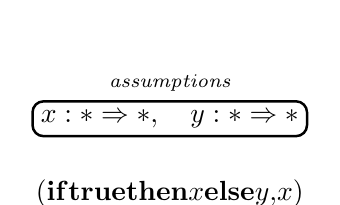
\begin{tikzpicture}[baseline=(t.base), every node/.style={inner sep=3pt}]
  \node[draw, line width=0.9pt, rounded corners,
        label={[font=\scriptsize\itshape]above:assumptions}] (a)
        {$x : \sPboth{\mathbf{*}\Rightarrow\mathbf{*}},\quad y : \sPtwo{\mathbf{*}\Rightarrow\mathbf{*}}$};
  \node[below=12pt of a] (t)
       {$\sPboth{(}\tokensp\sPboth{\mathbf{if}}\tokensp\mathbf{true}\tokensp\sPboth{\mathbf{then}}\tokensp\sPone{x}\tokensp\sPboth{\mathbf{else}}\tokensp\sPtwo{y}\tokensp\mathbf{,}\tokensp\sPboth{x}\tokensp\sPboth{)}$};
\end{tikzpicture}
\end{center}

\paragraph{Aliasing.} When this expression is embedded in the product $(\mathbf{if}\;\mathbf{true}\;\mathbf{then}\;x\;\mathbf{else}\;y,\; x)$, the outer use of $x$ \textit{joins} onto the assumption slice. As slices (A) (B) (C) each also use $x$, the assumptions are aliased, and in slices (A) (B) the assumptions now available in the if statement are strictly greater, making the expression non-minimal.

\paragraph{Proposal.} Use a stricter notion of synthesis slices that asks only ``is the term irreducible under the full assumptions $\Gamma$?''. Slices (A) and (B) are ruled out, but (C) and (D) are still valid. The next subsection makes this precise.

\subsection{\yo Term Slices}
\label{sec:term-minimal-slices}
\mechfile{Slicing/Synthesis/\\FixedAssmsSynthesis}

To rule out slices like (A) and (B) of Section~\ref{sec:product-revisited} we strengthen the notion of slice: rather than allowing the assumption context to vary across $\lfloor \Gamma \rfloor$, we fix it at the full $\Gamma$ and slice the term alone. The resulting slice is a sliced term that, under the original assumptions, still synthesises a type at least as precise as the query.

\begin{definition}[\yo Term-minimal slice]
\label{def:term-minimal-slice}
A \textit{term-minimal slice} of $D : \synthesis{e}{\tau}$ on $\upsilon \in \lfloor \tau \rfloor$, written $\tmslice{D}{\upsilon}$, is a triple, notated:
\[ \varsigma \mathbin{{\color{BrickRed}\Uparrow}} \psi \mathbin{\sqsupseteq} \upsilon \mathbin{\in} d \]
where $\varsigma \in \lfloor e \rfloor$ and derivation $d : \synthesis[\Delta;\,\Gamma]{\varsigma}{\psi}$ for $\psi \sqsupseteq \upsilon$, and $\psi \in \lfloor \tau \rfloor$ by graduality (Theorem~\ref{thm:graduality-syn}).
\end{definition}

\subsection{\yo Term-Minimality}
\label{sec:term-minimality}
\mechfile{Slicing/Synthesis/\\FixedAssmsSynthesis}

Minimality lifts directly from the slice lattice on $e$ alone:
\begin{definition}[\yo Minimal Term-Minimal Slices]
\label{def:mintmslice}
A $\mintmslice{D}{\upsilon}$ is a $\tmslice{D}{\upsilon}$ such that the term slice $\varsigma$ is minimal in $\{\varsigma \mid \varsigma \,{\color{BrickRed}\Uparrow}\, \psi \sqsupseteq \upsilon \in d : \tmslice{D}{\upsilon}\}$.
\end{definition}

The two notions of minimality do not coincide: term-minimality is strictly stronger. Not all minimal slices are term-minimal under maximal assumptions.

\begin{counterexamplebox}
\mechbox{\textnormal{\textbf{¬}}min-syn-is-\\min-fixedassms}%
\begin{counterexample}[\yo Minimal $\not\Rightarrow$ Term-Minimal]\label{lem:min-not-tmin}
Slices (A) and (B) of Section~\ref{sec:product-revisited} are minimal synthesis slices but not term-minimal.
\end{counterexample}
\end{counterexamplebox}

\subsection{\po Existence of Minimal Term-Minimal Slices}
\label{sec:tmin-exists}
\mechfile{Slicing/Synthesis/\\FixedAssmsSynthesis}

As with synthesis slices, every term-minimal slice has a minimal slice below it:

\mechbox{tmin-exists}%
\begin{theorem}[\po Existence of minimal term-minimal slices]\label{thm:tmin-exists}
For every $s : \tmslice{D}{\upsilon}$, there exists $m : \mintmslice{D}{\upsilon}$ with $m \sqsubseteq s$.
\end{theorem}

The rest of this chapter develops a structural calculus that characterises minimal term slices via a judgement:
\[ \Gamma \vdash e \mathbin{{\color{BrickRed}\Uparrow}} \tau \mathbin{\blacktriangleleft} \upsilon \;{\color{BrickRed}\rightsquigarrow}\; \varsigma \mathbin{{\color{BrickRed}\Uparrow}} \psi \dashv \gamma, \]
read ``the typing $\Gamma \vdash e \Uparrow \tau$ at query $\upsilon$ produces term slice $\varsigma$, synthesises $\psi$, and uses assumptions $\gamma$''. The fourth output $\gamma$ is a minimal assumption slice to retrieve a minimal slice corresponding to the term-minimal slice.

\subsection{\yo Term-Minimal $\to$ Minimal Slice}
\label{sec:tmin-to-min}
\mechfile{Slicing/Synthesis/\\FixedAssmsCalc}

Therefore, a minimal slice can be extracted from this by pairing $\gamma$ with $\varsigma$:

\begin{majortheorembox}
\mechbox{tmin-is-min}%
\begin{theorem}[\yo Soundness: term-minimal $\Rightarrow$ minimal]\label{thm:tmin-to-min}

If $\varsigma$ is a term-minimal slice on query $\upsilon$, then for any minimal context $\gamma$ for $\varsigma$ that still synthesises a more or equally less precise type to $\upsilon$, then $(\gamma, \varsigma$) is a minimal synthesis slice on $\upsilon$.
\end{theorem}
\end{majortheorembox}

\begin{proof}
The term component $\varsigma$ is minimal at full $\Gamma$, so is minimal \emph{a fortiori} at any $\gamma' \sqsubseteq \Gamma$ by graduality, hence is a MinSynSlice at the minimal context $\gamma$ produced by the calculus.
\end{proof}

This justifies the algorithmic strategy that occupies the rest of the chapter: compute term-minimal slices structurally, then promote them to full minimal slices.

\subsection{\yo Calculating Term-Minimal Slices}
\label{sec:term-minimal-calculus}
\mechfile{Slicing/Synthesis/\\FixedAssmsCalc}

As mentioned previously, restricting to term-minimality allows products to be calculated by pairing sub-slices at the corresponding sub-queries, i.e. for $\upsilon_1 \times \upsilon_2$, slice the first component at $\upsilon_1$, similarly for the second. More generally, if a typing rule has sub-terms which synthesise types, then recursively slice them. Otherwise, if a sub-term analyses against a type, it can be omitted entirely.

\begin{figure}[p]
\centering
\scriptsize
\fbox{\normalsize $\Delta;\,\Gamma \vdash e \Uparrow \tau \mathbin{\blacktriangleleft} \upsilon \rightsquigarrow \varsigma \Uparrow \psi \dashv \gamma$}
\bigskip

\inference[\synr{Var}]{
  \Gamma(x) = \tau \quad \upsilon \neq \gap
}{\tmrule{x}{\tau}{\upsilon}{x}{\tau}{\latticebot[x \mapsto \upsilon]}}

\bigskip

\inference[\synr{Gap}]{}{\tmrule{e}{\tau}{\gap}{\gap}{\gap}{\latticebot}}

\bigskip

\inference[\synr{Const}]{}{\tmrule{*}{*}{\latticetop}{*}{*}{\latticebot}}

\bigskip

\inference[\synr{Pair}]{
  \tmrule{e_1}{\tau_1}{\upsilon_1}{\varsigma_1}{\psi_1}{\gamma_1}
  &
  \tmrule{e_2}{\tau_2}{\upsilon_2}{\varsigma_2}{\psi_2}{\gamma_2}
}{\tmrule{(e_1, e_2)}{\tau_1 \times \tau_2}{\upsilon_1 \times \upsilon_2}{(\varsigma_1, \varsigma_2)}{\psi_1 \times \psi_2}{\gamma_1 \sqcup \gamma_2}}

\bigskip

\inference[\synr{Proj}]{
  \upsilon \neq \gap
  &
  \tmrule{e}{\tau_1 \times \tau_2}{\widehat{\upsilon}_i}{\varsigma}{\psi_1}{\gamma}
}{\tmrule{\pi_i\,e}{\tau_i}{\upsilon}{\pi_i\,\varsigma}{\pi_i\,\psi_1}{\gamma}}

\bigskip

\inference[\synr{App}]{
  \analysis{e_2}{\tau_1}
  &
  \upsilon \neq \gap
  &
  \tmrule{e_1}{\tau_1 \Rightarrow \tau_2}{\gap \Rightarrow \upsilon}{\varsigma_{\mathit{fn}}}{\psi_1}{\gamma}
}{\tmrule{e_1\,e_2}{\tau_2}{\upsilon}{\varsigma_{\mathit{fn}}(\gap)}{\mathsf{cod}(\psi_1)}{\gamma}}

\bigskip

\inference[\synr{Lam{:}}]{
  \tmrule[\Delta;\,\Gamma, x{:}\tau_1]{e_2}{\tau_2}{\upsilon_2}{\varsigma_2}{\psi_2}{\gamma, x{:}\phi_1}
  &
  \synthesis[\Delta;\,\Gamma, x{:}(\phi_1 \sqcup \upsilon_1)]{\varsigma_2{\downarrow}}{\psi_2'{\downarrow}}
}{\tmrule{\lambda x{:}\tau_1.\,e_2}{\tau_1 \Rightarrow \tau_2}{\upsilon_1 \Rightarrow \upsilon_2}{\lambda x{:}(\phi_1 \sqcup \upsilon_1).\;\varsigma_2}{(\phi_1 \sqcup \upsilon_1) \Rightarrow \psi_2'}{\gamma}}

\bigskip

\inference[\synr{Let}]{
  \upsilon_2 \neq \gap
  &
  \tmrule[\Delta;\,\Gamma, x{:}\tau_1]{e_2}{\tau_2}{\upsilon_2}{\varsigma_b}{\psi_2}{\gamma_2, x{:}\upsilon_1}
  &
  \tmrule{e_1}{\tau_1}{\upsilon_1}{\varsigma_d}{\psi_1}{\gamma_1}
  &
  \synthesis[\Delta;\,\Gamma, x{:}\psi_1]{\varsigma_b{\downarrow}}{\psi_2'{\downarrow}}
}{\tmrule{\mathbf{let}\;x = e_1\;\mathbf{in}\;e_2}{\tau_2}{\upsilon_2}{\mathbf{let}\;x = \varsigma_d\;\mathbf{in}\;\varsigma_b}{\psi_2'}{\gamma_1 \sqcup \gamma_2}}

\bigskip

\inference[\synr{TLam}]{
  \tmrule[\Delta, \alpha;\,\Gamma]{e}{\tau}{\upsilon}{\varsigma}{\psi'}{\gamma}
}{\tmrule{\Lambda\alpha.\,e}{\forall\alpha.\,\tau}{\forall\alpha.\,\upsilon}{\Lambda\alpha.\,\varsigma}{\forall\alpha.\,\psi'}{\gamma}}

\bigskip

\centerline{\normalsize \fbox{\synr{TApp}: see Section~\ref{sec:term-min-tapp}.}}

\bigskip

\centerline{\normalsize \fbox{\synr{Case}: see Section~\ref{sec:fixed-point}.}}
\caption{Term-minimal slice calculus rules.}
\label{fig:tmrules}
\end{figure}

\bigskip

\noindent The three cases that deserve commentary are the binders, the function application, and the type application; the \synr{Lam{:}}\ and \synr{Let}\ rules each carry a body re-typing premise (rightmost) which re-derives the body's typing under the binder slice $\gamma(x)$.

\subsubsection{\yo Function Application}
\label{sec:term-min-app}

For example, for function application, omit the argument, and slice the function by $\gap \Rightarrow \upsilon$, the argument type is not required to determine the return type:
\[
\inference[\synr{App}]{
  \analysis{e_2}{\tau_1}
  &
  \upsilon \neq \gap
  &
  \tmrule{e_1}{\tau_1 \Rightarrow \tau_2}{\gap \Rightarrow \upsilon}{\varsigma_{\mathit{fn}}}{\psi_1}{\gamma}
}{\tmrule{e_1\,e_2}{\tau_2}{\upsilon}{\varsigma_{\mathit{fn}}(\gap)}{\mathsf{cod}(\psi_1)}{\gamma}}
\]

\subsubsection{\yo Lambdas, Lets, and Type Abstractions}
\label{sec:term-min-binders}

Rules which bind variables are more complex, as they abstract a variable used in the minimised body. Slice them by first slicing the body, extracting the assumption it needed for the bound variable from $\gamma$, then slice the definition / type annotation using this. Notice that this is the \textit{opposite} direction to typechecking.\footnote{e.g. let bindings type the definition first, then use the result to type the body.}

\paragraph{Annotated lambda.} Set the annotation to $\gamma(x)$ where $\gamma$ is the chosen minimal assumptions for $x$ in slicing the body.\footnote{Assuming wlog. the variable bound by the function is $x$.}

\paragraph{Let bindings.} Slice the definition according to $\gamma(x)$.

\subsubsection{\yo Type Application}
\label{sec:term-min-tapp}

Type application works by matching the type function's type against the query to collect a list of constraints on the type variable, the \textit{join} of which gives the sliced type argument $\hat\sigma$. The type function is then sliced with a matched query $\widehat{\upsilon}$, where each $\alpha$-position of the query is replaced by $\alpha$ and non-$\alpha$ positions are carried through unchanged. Figure~\ref{fig:tapp-minsub} illustrates the construction on a query whose two $\alpha$-positions give differing constraints.

\begin{figure}[t]
\centering
$e \mathbin{{\color{BrickRed}\Uparrow}} \forall\alpha.\,(\alpha \times \alpha \times \mathbf{Bool})$,\quad applied at\quad $\sigma = \mathbf{*} \Rightarrow (\mathbf{Bool} \times \mathbf{Bool})$:

\medskip

\begin{tabular}{r@{\;\;}l}
\textbf{Query}             & $\upsilon \;=\; \underbrace{\sli[teal]{\mathbf{*} \Rightarrow \gap}}_{\alpha} \;\times\; \underbrace{\sli[teal]{\gap \Rightarrow (\mathbf{Bool} \times \gap)}}_{\alpha} \;\times\; \gap$ \\[16pt]
\textbf{Matched query}     & $\widehat{\upsilon} \;=\; \alpha \;\times\; \alpha \;\times\; \gap$ \\[8pt]
\textbf{Constraints}       & $\mathbf{*} \Rightarrow \gap \;\sqsubseteq\; \alpha \qquad \gap \Rightarrow (\mathbf{Bool} \times \gap) \;\sqsubseteq\; \alpha$ \\[8pt]
\textbf{Constraints Join}  & $\hat\sigma \;=\; \mathbf{*} \Rightarrow (\mathbf{Bool} \times \gap)$ \\
\end{tabular}
\caption{Type application.}
\label{fig:tapp-minsub}
\end{figure}

\subsection{\no Fixed Point Algorithm for Case Expressions}
\label{sec:fixed-point}
\mechfile{Slicing/Synthesis/\\CaseAlgorithm}

\noindent This is the complex case, minimal slices must have no redundant type information from both branches, so the query must be split between the branches. However, simply splitting the query disjointly between the branches is not enough to ensure minimality.

\paragraph{The Overlap Problem.} Suppose a case expression $\mathbf{case}\;e\;\mathbf{of}\;x.\,e_1 \mid y.\,e_2$ synthesises $\tau_1 \sqcup \tau_2$. Suppose we disjointly split a query $\upsilon \in \lfloor \tau_1 \sqcup \tau_2$ into $\upsilon_1 \in \lfloor \tau_1 \rfloor$ and $\upsilon_2 \in \lfloor \tau_2 \rfloor$. Then slice the branches, but as minimal slices are not necessarily exact (\cref{lem:exact-not-exist}), then they may synthesise strictly more prescise $\psi_1$ and $\psi_2$. In this situation, branch 1 actually only needed to cover what $\psi_2$ didn't cover, which is stricly less than the $\upsilon_1$ it was queried under, so it may not be minimal on this, and vice versa for branch 2.
\begin{figure}[!htb]
\centering
\begin{subfigure}[t]{0.48\textwidth}\centering
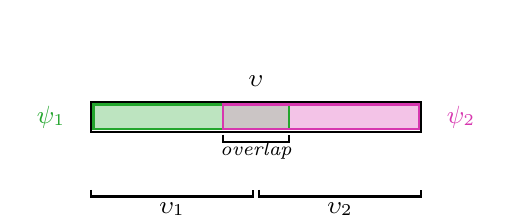
\begin{tikzpicture}[every node/.style={font=\small}, scale=0.7]
  \draw[thick] (0,0) rectangle (6,0.55);
  \fill[OliveGreen!30] (0.05,0.05) rectangle (2.4,0.5);
  \fill[OliveGreen!50!Mulberry!40] (2.4,0.05) rectangle (3.6,0.5);
  \fill[Mulberry!30]   (3.6,0.05) rectangle (5.95,0.5);
  \draw[OliveGreen,thick] (0.05,0.05) rectangle (3.6,0.5);
  \draw[Mulberry,thick]   (2.4,0.05) rectangle (5.95,0.5);
  \node[above=2pt of {(3,0.55)}] {$\upsilon$};
  \node[OliveGreen, left=2mm of {(0,0.275)}, font=\small\itshape] {$\psi_1$};
  \node[Mulberry, right=2mm of {(6,0.275)}, font=\small\itshape] {$\psi_2$};
  \draw[thick] (2.4,-0.05) -- (2.4,-0.18) -- (3.6,-0.18) -- (3.6,-0.05);
  \node[font=\scriptsize\itshape] at (3.0,-0.34) {overlap};
  \draw[thick] (0,-1.05) -- (0,-1.17) -- (2.95,-1.17) -- (2.95,-1.05);
  \node at (1.475,-1.40) {$\upsilon_1$};
  \draw[thick] (3.05,-1.05) -- (3.05,-1.17) -- (6,-1.17) -- (6,-1.05);
  \node at (4.525,-1.40) {$\upsilon_2$};
\end{tikzpicture}
\caption{Disjoint split.}
\label{fig:case-overlap-disjoint}
\end{subfigure}\hfill
\begin{subfigure}[t]{0.48\textwidth}\centering
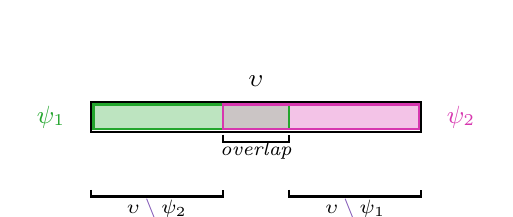
\begin{tikzpicture}[every node/.style={font=\small}, scale=0.7]
  \draw[thick] (0,0) rectangle (6,0.55);
  \fill[OliveGreen!30] (0.05,0.05) rectangle (2.4,0.5);
  \fill[OliveGreen!50!Mulberry!40] (2.4,0.05) rectangle (3.6,0.5);
  \fill[Mulberry!30]   (3.6,0.05) rectangle (5.95,0.5);
  \draw[OliveGreen,thick] (0.05,0.05) rectangle (3.6,0.5);
  \draw[Mulberry,thick]   (2.4,0.05) rectangle (5.95,0.5);
  \node[above=2pt of {(3,0.55)}] {$\upsilon$};
  \node[OliveGreen, left=2mm of {(0,0.275)}, font=\small\itshape] {$\psi_1$};
  \node[Mulberry, right=2mm of {(6,0.275)}, font=\small\itshape] {$\psi_2$};
  \draw[thick] (2.4,-0.05) -- (2.4,-0.18) -- (3.6,-0.18) -- (3.6,-0.05);
  \node[font=\scriptsize\itshape] at (3.0,-0.34) {overlap};
  \draw[thick] (0,-1.05) -- (0,-1.17) -- (2.4,-1.17) -- (2.4,-1.05);
  \node[font=\scriptsize] at (1.2,-1.40) {$\upsilon \heytingminus \psi_2$};
  \draw[thick] (3.6,-1.05) -- (3.6,-1.17) -- (6,-1.17) -- (6,-1.05);
  \node[font=\scriptsize] at (4.8,-1.40) {$\upsilon \heytingminus \psi_1$};
\end{tikzpicture}
\caption{Residual queries.}
\label{fig:case-overlap-residual}
\end{subfigure}
\caption{Abstract View of Overlap and Residuals.}
\label{fig:case-overlap}
\end{figure}

\subsubsection{Branch Residuals}
\label{sec:case-phase1}
When exactly are two branch slices jointly minimal? Let $\upsilon_1$ and $\upsilon_2$ be the branch queries, then when (see Figure~\ref{fig:case-overlap-residual}):
\begin{itemize}
\item $\upsilon_1 \sqsubseteq \upsilon \heytingminus \psi_2$. Branch 1 is queried on not more than is \textit{actually} provided by branch 2 or contained within $\upsilon$.
\item $\upsilon_2 \sqsubseteq \upsilon \heytingminus \psi_1$. Branch 2 is queried on not more than is \textit{actually} provided by branch 1 or contained within $\upsilon$.
\item $\upsilon \sqsubseteq \psi_1 \sqcup \psi_2$. The joined branch types actually cover the query.
\end{itemize}
It is still possible for $\psi_1$ and $\psi_2$ to overlap, but any overlap is not contained in the queries, so the branches are still minimal.
 
\paragraph{Iteration.} However, these are \textit{mutually dependent} slices, so they need iteration to solve. Let $\upsilon_1^i$ be the query on the $i$th iteration, $(\sigma_1^i, \psi_1^i)$ be the resulting slice and similarly for branch 2. Then iterate setting $\upsilon_1^1 = \upsilon \heytingminus \psi_2^0$, then setting $\upsilon_2^1 = \upsilon \heytingminus \psi_1^1$. Starting at $(\psi_1^0, \psi_2^0) = (\top, \gap)$.
\begin{figure}[!htb]
\centering
\begin{tikzpicture}[
  font=\small, >=stealth,
  every node/.style={inner sep=2pt},
  arr/.style={->, dashed, thick, shorten <=2pt, shorten >=2pt},
  arrass/.style={->, dashed, thick, shorten <=2pt, shorten >=2pt, draw=assumed}
]
  \node (a1) at (0,0)   {$\upsilon_1^1 := \upsilon \heytingminus \psi_2^0 \;\rightsquigarrow\; (\sigma_1^1, \psi_1^1)$};
  \node (b1) at (5.5,-1) {$\upsilon_2^1 := \upsilon \heytingminus \psi_1^1 \;\rightsquigarrow\; (\sigma_2^1, \psi_2^1)$};
  \node (a2) at (0,-2)  {$\upsilon_1^2 := \upsilon \heytingminus \psi_2^1 \;\rightsquigarrow\; (\sigma_1^2, \psi_1^2)$};
  \node (b2) at (5.5,-3) {$\upsilon_2^2 := \upsilon \heytingminus \psi_1^2 \;\rightsquigarrow\; (\sigma_2^2, \psi_2^2)$};
  \node (dots) at (2.75,-4) {$\vdots$};
  \draw[arrass] (a1.south east) -- (b1.north west);
  \draw[arr]    (b1.south west) -- (a2.north east);
  \draw[arrass] (a2.south east) -- (b2.north west);
  \draw[arr]    (b2.south west) -- (dots.north east);
  \node[assumed] (p20) at (10.5, 0)  {$\psi_2^0$};
  \node[assumed] (p21) at (10.5,-1) {$\psi_2^1$};
  \node[assumed] (p22) at (10.5,-3) {$\psi_2^2$};
  \node[assumed] (p2d) at (10.5,-4) {$\cdots$};
  \node[assumed] at ($(p20)!0.5!(p21)$) {\rotatebox{-90}{$\sqsubseteq$}};
  \node[assumed] at ($(p21)!0.5!(p22)$) {\rotatebox{-90}{$\sqsubseteq$}};
  \node[assumed] at ($(p22)!0.5!(p2d)$) {\rotatebox{-90}{$\sqsubseteq$}};
  \node[assumed, font=\scriptsize\itshape, above=1mm of p20] {(assumed)};
\end{tikzpicture}
\caption{Branch Fixed Point Iteration}
\label{fig:case-iteration}
\end{figure}
We wish to show that $\psi_1$ decreases monotonically and $\psi_2$ increases monotonically.

As co-Heyting subtraction is anti-monotone in its second argument (\cref{lem:heyt-mono}), then as $\psi_2$ increases,\footnote{All use of increase/decrease here is in the monotonic sense.} $\upsilon_1$ decreases and as $\psi_1$ decreases, $\upsilon_2$ increases. At the start, $\psi_2^0 = \gap$, so $\psi_2$ increases on the first step, so $\upsilon_1$ decreases on the first step.

By monotonicity of minimum synthesis slices (\cref{thm:mono}), we can find $\sigma_1$ decreasing and hence $\psi_1$ decreasing. Hence, $\upsilon_2$ increases (by anti-monotonicity). However, an upwards monotonicity theorem, which would conclude the next step, that $\psi_2$ monotonically increases, does \textit{not} hold (\cref{lem:dual-mono-fails}). But, when it does, $\upsilon_1$ would decrease inductively, completing the loop. 

Hence, \textit{when the chain $\psi_2$ monotonically increases}, then $\psi_1$ monotonically decreases. So, by Kleene's finite fixed point theorem (\cref{thm:kleene}) this iteration leads to a fixed point with $\upsilon_1 = \upsilon \heytingminus \psi_2$ and $\upsilon_2 \heytingminus \psi_1$, satisfying the first two constraints for jointly minimal branches. And as $\upsilon \sqsubseteq \psi_1$ and $\upsilon_2 \sqsubseteq \psi_2$ by validity of synthesis slices, then the third condition holds $\upsilon \sqsubseteq \psi_1 \sqcup \psi_2$ by the co-Heyting algebra properties.

\begin{counterexamplebox}
\mechbox{\textnormal{\textbf{¬}}upward-closure-\\min-fixedassms}%
\begin{counterexample}[\yo Upwards Non-Monotonicity]\label{lem:dual-mono-fails}
For $\Gamma = (z : \mathbf{*}\times\mathbf{*})$ and $D : \synthesis{\mathbf{if}\;\gap\;\mathbf{then}\;z\;\mathbf{else}\;(\mathbf{*}, \gap)}{\mathbf{*}\times\mathbf{*}}$, the unique minimal slices at $\upsilon = \mathbf{*}\times\mathbf{*}$ and $\upsilon' = \mathbf{*}\times\gap$ are incomparable:
\begin{center}
\fullslice{z : \sli{\mathbf{*}\times\mathbf{*}}}{\sli{\mathbf{if}}\;\gap\;\sli{\mathbf{then}\;z\;\mathbf{else}}\;\gap}
\quad$\not\sqsupseteq$\quad
\fullslice{z : \gap}{\sli{\mathbf{if}}\;\gap\;\sli{\mathbf{then}}\;\gap\;\sli{\mathbf{else}\;(\mathbf{*}, \gap)}}
\end{center}
\end{counterexample}
\end{counterexamplebox}

Therefore, this part of the algorithm is partial. In reality, this covers most cases, and you can revert to the brute force algorithm otherwise. Devising a complete (non-brute force) algorithm is left to future work. Another potential downside of this algorithm is that it is \textit{biased}, it prefers to select typing information from branch 1.

\subsubsection{Scrutinee Descent}
\label{sec:case-phase2}

The branches are now jointly minimal under the full context. But, case statements also include \textit{bindings}, whose type are sourced by another term. However, unlike with let bindings, we can't simply take the minimal assumptions of the branches, because those may only provide enough to synthesise the residual queries $\upsilon_i$, which may not cover the original query $\upsilon$.\footnote{We only have that $\upsilon \sqsubseteq \psi_1 \sqcup \psi_2$.}

As case scrutinee terms are typically small in real world code (e.g. if statements), we can simply do a brute-force descent on the scrutinee. But, if the term is significantly larger than the type, it makes sense to can perform a brute-force descent on the bound types to find a minimal pair of assumptions to cover the query $\upsilon$: that is, $x : \phi_1; \Gamma \vdash \sigma_1 \vdash \psi_1'$ and $y : \phi_2; \Gamma \vdash \sigma_2 \vdash \psi_2'$ with $\upsilon \sqsubseteq \psi_1' \sqcup \psi_2'$. Then slice the scrutinee according to $\phi_1 + \phi_2$ and use this as a smaller starding point to descend on. 

\subsubsection{The Assumption Slice}
\label{sec:case-phase3}

At this point we have a term-minimal slice, but we still need a minimal assumption slice. Again, this does not directly follow from the minimal assumptions for the branches individually, due to \textit{aliasing} of common assumptions. However, you can join these individual minima alongside the minimal assumptions for the scrutinee (calculated by brute-force\footnote{\textit{Ascending} from $\emptyset$ being more efficient here.} or over-approximated using the slice on $\phi_1 + \phi_2$). This gives a set of valid assumptions to synthesise $\upsilon$ which will be \textit{near-minimum} and work as a good starting point to brute-force from.

\subsection{\po Calculating Analysis Slices}
\label{sec:ana-slice-calculus}
\mechfile{Slicing/Analysis/\\AnaSliceCalc}

Analysis slices work on context classifications, and a similar judgement can be defined, but upon context:
\[ \mathit{Cls} \mathbin{\blacktriangleleft} \upsilon \;\rightsquigarrow\; (\kappa,\,\gamma,\,\psi), \]
producing a context slice $\kappa \in \lfloor\C\rfloor$, an assumption slice $\gamma \in \lfloor\Gamma\rfloor$, and an \textit{induced outer slice} $\psi \in \lfloor\tau_p\rfloor$ -- the slice of the outer-derivation type $\tau_p$ that the resulting context slice $\kappa$ produces (the synthesis-slice analogue of $\phi$ in Section~\ref{sec:syn-slice-def}). I give the two most interesting cases: function application, which makes use of a synthesis slice, and unannotated lambdas.

\paragraph{Function application ($e \circ_2 \C$).} Recursively slice the argument context $\C$ at $\upsilon$ to obtain its induced outer slice $\upsilon' \in \lfloor\tau_1\rfloor$, then synthesis-slice the function $e$ at the arrow query $\upsilon' \Rightarrow \gap$. The codomain of the function's sliced arrow type is the application's induced outer slice.

\paragraph{Unannotated lambda ($\lambda x.\,\C$).} The body recurses; its used-assumption slice decomposes as $\gamma', x{:}\hat\tau_1$, with $\hat\tau_1 \in \lfloor\tau_1\rfloor$ the binder's slice. The induced outer slice is the arrow $\hat\tau_1 \Rightarrow \upsilon'$:
{\small
\[
\inference[$\mathit{minA\lambda{\Rightarrow}}$]
  {\tau \sqcup \gap \Rightarrow \gap \equiv \tau_1 \Rightarrow \tau_2
   &
   \overbrace{\ctxclass[\Delta;\,\Gamma,\, x{:}\tau_1]{\C}{{\color{BlueViolet}\Downarrow}\,\tau_2}{\Delta';\,\Gamma'}{{\color{BlueViolet}\Leftarrow}\,\tau_f}}^{\textstyle\mathit{Cls}'}
   \mathbin{\blacktriangleleft} \upsilon \rightsquigarrow (\kappa',\,(\gamma', x{:}\hat\tau_1),\,\upsilon')}
  {\underbrace{\ctxclass{\lambda x.\,\C}{{\color{BlueViolet}\Downarrow}\,\tau}{\Delta';\,\Gamma'}{{\color{BlueViolet}\Leftarrow}\,\tau_f}}_{\textstyle \lambda x.\,\mathit{Cls}'}
   \mathbin{\blacktriangleleft} \upsilon \rightsquigarrow
   (\lambda x.\,\kappa',\;\gamma',\;\hat\tau_1 \Rightarrow \upsilon')}
\]
}

%%% Local Variables:
%%% mode: LaTeX
%%% TeX-master: "PolymorphicTypeSlicing"
%%% End:

\section{\no Minimum-Size Slicing}
\label{sec:complexity}

\sectionlegend

We can calculate a \textit{minimal} synthesis slice in polynomial time (\cref{sec:min-exists}). However, minimal slices are not unique, so a natural extension is to rank them by \textit{size} and ask for a minimal slice of \textit{minimum size}. This chapter reduces the \textit{set cover optimisation problem} to calculating minimum size slice, meaning minimum-size slicing is \textbf{NP-hard}. I (informally) prove this for term-minimal synthesis slices, and show that the argument extends to general minimal synthesis slices and to analysis slices.

\subsection{\no Definitions}\label{sec:complexity-setup}

\begin{definition}[Size of an Expression Slice]\label{def:slice-size}
For an expression slice $\varsigma \in \lfloor e \rfloor$, the size $|\varsigma|$ counts non-$\gap$ syntactic positions:
\[
  |\gap| = 0,\qquad |*| = 1,\qquad |x| = 1, \qquad |c(\varsigma_1, \dots, \varsigma_k)| = 1 + \textstyle\sum_i |\varsigma_i|.
\]
\end{definition}

\begin{definition}[\textsc{Minimum-Size TermMinimal Slice Problem}]\label{def:min-tm-slice}
Given a derivation $D : \synthesis{e}{\tau}$ and query $\upsilon \in \lfloor\tau\rfloor$, the minimum-size term-minimal slice problem is to compute
\[
  \mathrm{minSize}(D, \upsilon) \;\triangleq\; \min\bigl\{\,|\sigma| \;:\; \sigma \in \tmslice{D}{\upsilon}\,\bigr\}.
\]
\end{definition}

\begin{definition}[\textsc{Minimum Set Cover (Optimisation) Problem}]\label{def:min-set-cover}
Given a universe $U = \{1, \dots, n\}$ and a family $S = S_1, \dots, S_m \subseteq U$, compute
\[
  K^\star(U, S) \;\triangleq\; \min\bigl\{\,|J| \;:\; J \subseteq \{1, \cdots, m\},\; \textstyle\bigcup_{j \in J} S_j = U\,\bigr\}.
\]
\end{definition}

The minimum set cover optimisation problem is NP-hard~\cite[\S16.1, p.~414]{KorteVygen}, hence any polynomial reduction from it, is also NP-hard.

\subsection{\no The reduction}\label{sec:complexity-reduction}

\begin{definition}[Reduction to Min-set-cover]\label{def:reduction}
Given an instance $(U, S_1, \dots, S_m)$ of \textsc{Min-Set-Cover}, suppose wlog. $|U| = n$ and $\bigcup_j S_j = U$. Then construct $D : \synthesis{e}{\tau}$ and query $\upsilon = \tau$ as follows:
\begin{itemize}
\item \textbf{Target type $\tau$:} $\tau \;=\; \underbrace{*\,\times\,(*\,\times\,(\cdots \times (*\,\times\,*)))}_{n \text{ projections}}$. Position $i$ of $\tau$ corresponds to element $i$ of $U$.
\item \textbf{Encoding $S_j \mapsto T_j$:} For each $j$, construct type slice family $T_j \in \lfloor\tau\rfloor$ by omitting all projections $i$ for $i \not\in S_j$. Then $\bigsqcup_{j} T_j = \tau$ iff $\bigcup_j S_j = U$, where $\bigsqcup_j$ is the finite join of family $T_j$.
\item \textbf{Assumption context $\Gamma$:} $\Gamma \;=\; (x_1 : T_1,\; \dots,\; x_m : T_m)$, so each $x_j$ synthesises $T_j$ exactly under \synr{Var}.
\item \textbf{Case tree $e$:} Construct any binary case tree with leaves $x_1, \dots, x_m$, and having all scrutiness being $\gap$ and all binders being $x$.

By \cref{lem:slices-consistent} the leaves' synthesised types are mutually consistent, so the case rule applies at every node, giving $\synthesis{e}{\bigsqcup_j T_j} = \synthesis{e}{\tau}$. The tree has size $|e| = 2m - 1$: $m$ leaves and $m-1$ case expressions.
\item \textbf{Query:} $\upsilon = \tau$.
\end{itemize}
\end{definition}

\noindent This construction is trivially computable in polynomial (linear) time: $\mathcal{O}(n + m + \sum_{j}{|S_j|}).$

Concretely, view each set $S_j$ as a \textit{variable} $x_j$ whose type is a slice of the target carrying $*$ exactly where $S_j$ has an element. Then any slice of the case tree $e$ represents a choice of variables $x_j$. \Cref{fig:set-cover-case-tree} draws this correspondence on a $4$-element universe.

\begin{figure}[ht]
\centering
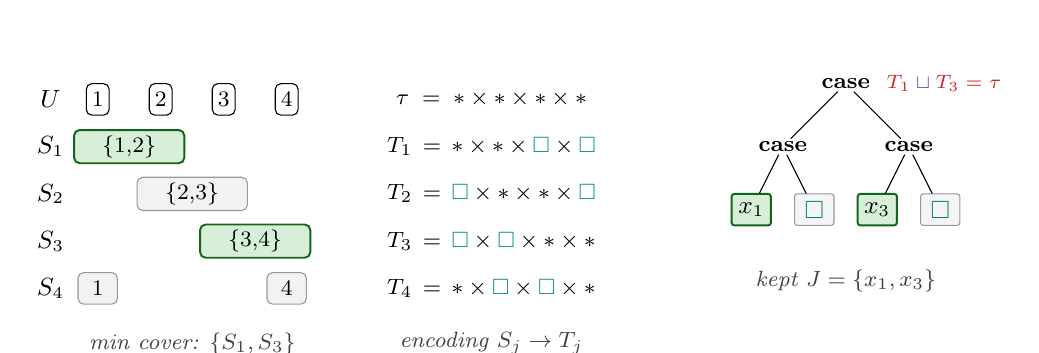
\begin{tikzpicture}[
    sc/.style={draw, rounded corners=2pt, inner sep=2pt, minimum height=4mm, font=\footnotesize},
    sel/.style={fill=OliveGreen!18, draw=OliveGreen!60!black, line width=0.7pt},
    no/.style={fill=black!5, draw=black!40},
    ca/.style={font=\bfseries\footnotesize, inner sep=1pt},
    lf/.style={draw, rounded corners=1pt, inner sep=2pt, minimum width=5mm, minimum height=4mm, font=\small},
    kp/.style={draw=OliveGreen!60!black, fill=OliveGreen!18, line width=0.7pt},
    dr/.style={draw=black!40, fill=black!4, text=black!50},
    every node/.append style={font=\small},
    line cap=round]

\node[font=\itshape\small] at (-0.6,0.6) {$U$};
\node[sc] at (0.0,0.6) {1};
\node[sc] at (0.8,0.6) {2};
\node[sc] at (1.6,0.6) {3};
\node[sc] at (2.4,0.6) {4};

\node[font=\itshape\small] at (-0.6,0.0) {$S_1$};
\node[sc, sel, minimum width=14mm] at (0.4,0.0) {\{1,2\}};
\node[font=\itshape\small] at (-0.6,-0.6) {$S_2$};
\node[sc, no,  minimum width=14mm] at (1.2,-0.6) {\{2,3\}};
\node[font=\itshape\small] at (-0.6,-1.2) {$S_3$};
\node[sc, sel, minimum width=14mm] at (2.0,-1.2) {\{3,4\}};
\node[font=\itshape\small] at (-0.6,-1.8) {$S_4$};
\node[sc, no,  minimum width=5mm]  at (0.0,-1.8) {1};
\node[sc, no,  minimum width=5mm]  at (2.4,-1.8) {4};

\node[font=\footnotesize\itshape, text=gray!50!black, align=center] at (1.2,-2.5)
  {min cover: $\{S_1,S_3\}$};

\node[font=\footnotesize, align=left] at (5.0,0.6)  {$\tau \;=\; * \times * \times * \times *$};
\node[font=\footnotesize, align=left] at (5.0,0.0)  {$T_1 \,=\, * \times * \times \gap \times \gap$};
\node[font=\footnotesize, align=left] at (5.0,-0.6) {$T_2 \,=\, \gap \times * \times * \times \gap$};
\node[font=\footnotesize, align=left] at (5.0,-1.2) {$T_3 \,=\, \gap \times \gap \times * \times *$};
\node[font=\footnotesize, align=left] at (5.0,-1.8) {$T_4 \,=\, * \times \gap \times \gap \times *$};
\node[font=\footnotesize\itshape, text=gray!50!black, align=center] at (5.0,-2.5)
  {encoding $S_j \to T_j$};

\node[ca] (rt) at (9.5, 0.8) {case};
\node[ca] (cl) at (8.7, 0.0) {case};
\node[ca] (cr) at (10.3,0.0) {case};
\node[lf, kp] (l1) at (8.3,-0.8) {$x_1$};
\node[lf, dr] (l2) at (9.1,-0.8) {$\gap$};
\node[lf, kp] (l3) at (9.9,-0.8) {$x_3$};
\node[lf, dr] (l4) at (10.7,-0.8) {$\gap$};
\draw (rt) -- (cl);
\draw (rt) -- (cr);
\draw (cl) -- (l1);
\draw (cl) -- (l2);
\draw (cr) -- (l3);
\draw (cr) -- (l4);
\node[font=\scriptsize, text=BrickRed, anchor=west] at (rt.east) {\,$T_1 \sqcup T_3 = \tau$};
\node[font=\footnotesize\itshape, text=gray!50!black, align=center] at (9.5,-1.7)
  {kept $J = \{x_1, x_3\}$};

\end{tikzpicture}
\caption{Set cover (left), the encoding (middle), and the induced case-tree slice (right), with a minimal set cover selected.}
\label{fig:set-cover-case-tree}
\end{figure}

\subsection{\no Correctness}\label{sec:complexity-correctness}

Throughout this subsection, write $J(\sigma) = \{j : x_j \in \varsigma\}$ for the set of leaves retained in a slice $\sigma$ of $e$.

\begin{lemma}[Validity is Set-Cover]\label{lem:tm-validity}
A term-minimal slice $\sigma$ of $D$ at $\upsilon = \tau$ is valid iff $J(\sigma)$ is a set cover of $U$.
\end{lemma}

\begin{proof}
Under fixed $\Gamma$, $x_j$ in the slice synthesises $T_j$ (rule \synr{Var}), and a $\gap$-leaf synthesises $\gap$. Walking up the case tree, the case rule joins branch types pointwise, so $\sigma$ synthesises $\bigsqcup_{j \in J(\sigma)} T_j$. Validity ($\sqsupseteq \tau$) holds iff every position of $\tau$ is covered. As $\tau$ encodes $U$, then validity holds iff $\bigcup_{j \in J(\sigma)} S_j = U$.
\end{proof}

\begin{lemma}[Minimum Set Size]\label{lem:tm-size}
For $(\Gamma, e, \tau)$ encoding Min-Set-Cover problem $(U, S)$. From minSize$(\synthesis{e}{\tau}, \tau)$ we can calculate $K^{\star}(U, S)$ in polynomial time.
\end{lemma}

\begin{proof}
Recurse once through minSize$(\synthesis{e}{\tau}, \tau)$ and count the number of variables, this is $|J(\sigma)| = K^{\star}(U,S)$. As $\sigma \sqsubseteq e$, then $|\sigma| \leq |e| = 2m - 1$, hence time complexity of this is $\mathcal{O}(m)$.
\end{proof}

\begin{majortheorembox}
\begin{theorem}[\textsc{Minimum-Size Term-Minimal-Slicing} is NP-hard]\label{thm:tm-min-nph}
Computing $\mathrm{minSize}(D, \upsilon)$ is NP-hard.
\end{theorem}
\end{majortheorembox}

\begin{proof}
Definition~\ref{def:reduction} is a polynomial-time many-one reduction from \textsc{Min-Set-Cover} to \textsc{Min-TM-Slice}, and Lemma~\ref{lem:tm-size} recovers $K^\star(U, S)$ from $\mathrm{minSize}(D, \upsilon)$ in polynomial time. Hence \textsc{Min-Set-Cover} $\le_p$ \textsc{Min-TM-Slice}, and NP-hardness of \textsc{Min-Set-Cover}~\cite[\S16.1, p.~414]{KorteVygen} transfers.
\end{proof}

\subsection{\no Extension to Min-Syn-Slice}\label{sec:min-syn-extension}

The reduction above can be embedded also into minimum synthesis slices, by forcing the minimal assumptions slice to be full by producting the case tree with all the variables $x_j$ and querying each set in this product fully.

\begin{definition}[Reduction to Min-Syn-Slice]\label{def:syn-reduction}
Let $(\Gamma, e_0, \tau)$ be the term-minimal encoding of Definition~\ref{def:reduction}. Form the product expression and query
\[
  e \;\triangleq\; (e_0,\, x_1,\, x_2,\, \dots,\, x_m),
  \qquad
  \upsilon \;\triangleq\; \tau \times T_1 \times T_2 \times \cdots \times T_m,
\]
under the same assumption context $\Gamma = (x_1 : T_1, \dots, x_m : T_m)$.
\end{definition}

\begin{lemma}[Maximal Assumption Slice]\label{lem:forced-gamma}
For every valid slice $\rho = (\gamma, \varsigma)$ of $\synthesis{e}{\upsilon}$ at $\upsilon$, $\gamma = \Gamma$.
\end{lemma}

\begin{proof}
The $(j+1)$-th projection is $x_j$ and is queried at $T_j$. This projection must synthesise $T_j$ under $\gamma$ via \synr{Var}. Hence, we require $\gamma(x_j) = T_j$, so $\gamma = \Gamma$.
\end{proof}

\begin{majortheorembox}
\begin{theorem}[\textsc{Minimum-Size Syn-Slice} is NP-hard]\label{thm:syn-min-nph}
Computing $\min\{|\rho| : \rho \in \synslice{D}{\upsilon}\}$ is NP-hard.
\end{theorem}
\end{majortheorembox}

\begin{proof}
By Lemma~\ref{lem:forced-gamma}, $|\gamma| = |\Gamma|$ is fixed by the input, and the outer-tuple variable positions $x_1, \dots, x_m$ contribute a further fixed $m$. Hence $|\rho| = |\Gamma| + m + |\varsigma_0|$, where $\varsigma_0$ slices the case-tree component $e_0$, and minimising $|\rho|$ reduces to the term-minimal problem on $(e_0, \tau)$. The construction is polynomial in $n + m$, and NP-hardness transfers from Theorem~\ref{thm:tm-min-nph}.
\end{proof}

%%% Local Variables:
%%% mode: LaTeX
%%% TeX-master: "PolymorphicTypeSlicing"
%%% End:

\section{Relation to Other Forms of Slicing}
\label{sec:comparisons}

Program slicing of various different forms, relating to dynamic execution, data dependencies, and type errors, has been studied extensively. In this chapter I compare type slicing with three other program slicing traditions: classical \emph{program slicing}~\cite{Weiser1984,TipSurvey1995}, \emph{Galois slicing}~\cite{Perera2012}, and \emph{type error slicing}~\cite{Wand1986,HaackWells2003}. Type slicing differs from all three, but has some similarities to Galois slicing.

\subsection{Classical Program Slicing}
\label{sec:cmp-program-slicing}

Classical program slicing \cite{Weiser1984,TipSurvey1995} was developed for imperative programs. Slices are syntactically obtained by deleting lines in the code, which is less flexible than omitting arbitrary sub-terms in a syntax tree as used here. The equivalent of type queries is a `slicing criterion', which is a (program-point, variable) pair, with the slice preserving the runtime value of the chosen variable at the chosen point. Type queries have a more complex, compound structure as compared to simple variables, and slices cannot preserve the type query in general (\cref{lem:exact-not-exist}), so we adopt the notion of \textit{validity} instead of preservation.

Program slicing has static and dynamic variants~\cite{Weiser1984,KorelLaski1988}, depending on whether the slicing criterion is preserved over \textit{all} inputs to the program or a particular execution. As typing is deterministic (\cref{thm:unicity}), this distinction does not apply to type slicing.

\subsection{Galois Slicing}
\label{sec:cmp-galois}

Galois slicing~\cite{Perera2012} is a lattice-theoretic version of type slicign that has subsequently been applied and related to a wide range of calculi and user interfaces~\cite{Ricciotti2017,PereraGarg2016,PereraVis2022,AtkeyPerera2025}.

Type slicing is related in the use of lattices and precision. However, Galois slices define a Galois connection, which unfortunately does not exist for type slicing.

\subsubsection{Background: Galois connections and the adjoint functor theorem}
\label{sec:cmp-galois-aft}

For context, an order-theoretic Galois connection is defined as follows:

\begin{definition}[Galois connection]
Let $(P, \sqsubseteq_P)$ and $(Q, \sqsubseteq_Q)$ be posets. A pair of monotone maps $f : P \to Q$ and $g : Q \to P$ is a \emph{Galois connection}, written $f \dashv g$ with $f$ the lower adjoint and $g$ the upper adjoint, when for every $p \in P$ and $q \in Q$
\[
  f(p) \sqsubseteq_Q q \iff p \sqsubseteq_P g(q).
\]
\end{definition}

\begin{proposition}[Adjoint Functor Theorem for Complete Lattices~{\cite[Prop.~7.34]{DaveyPriestley}}]
Let $P, Q$ be complete lattices. A monotone map $g : Q \to P$ is the upper adjoint of a (necessarily unique) Galois connection if and only if $g$ preserves all meets. When $g$ preserves meets, the lower adjoint $f$ is given pointwise by
\[
  f(p) = \bigsqcap \{\, q \in Q \mid g(q) \sqsupseteq p \,\}.
\]
\end{proposition}

\subsubsection{Slicing}
\label{sec:cmp-galois-perera}

Perera et al.\ work in a functional setting in which a program $e$ is evaluated under an environment $\rho$ to a value $v$, written $\rho, e \downdownarrows v$. For a fixed such terminating execution, they form the slice lattice $\lfloor \rho, e \rfloor$ of partial programs below $(\rho, e)$ and the slice lattice $\lfloor v \rfloor$ of partial values below $v$ (Perera et al.\ refer to these as prefixes, $\mathrm{Prefix}(\rho, e)$ and $\mathrm{Prefix}(v)$). Type slices have the same shape as Perera's slices: a partial program (here the slice $\rho$) paired with a partial value (here the synthesised type $\psi$), mediated by a derivation (here the typing derivation).

Restricted to the slice lattice below the executed program, evaluation lifts to a function
\[
  \mathit{eval}_{\rho,e} : \lfloor \rho, e \rfloor \to \lfloor v \rfloor
\]
which is total, monotone, and crucially meet-preserving:
\[
  \mathit{eval}_{\rho,e}(p_1 \sqcap p_2) = \mathit{eval}_{\rho,e}(p_1) \sqcap \mathit{eval}_{\rho,e}(p_2).
\]

By the adjoint functor theorem, $\mathit{eval}_{\rho,e}$ is then the upper adjoint of a unique Galois connection, with lower adjoint
\[
  \mathit{uneval}_{\rho,e} : \lfloor v \rfloor \to \lfloor \rho, e \rfloor,
  \qquad
  \mathit{uneval}_{\rho,e}(u) = \bigsqcap \{\, p \in \lfloor \rho, e \rfloor \mid \mathit{eval}_{\rho,e}(p) \sqsupseteq u \,\}
\]
This $\mathit{uneval}_{\rho,e}$ is the `backward slice function': it sends a partial-value query $u$ to the meet of all slices whose evaluation suffices to produce $u$, and that meet is itself in the set, so $\mathit{uneval}_{\rho,e}(u)$ is a least slice for $u$.

\subsubsection{Failure of Meet-Preservation for Type Synthesis}
\label{sec:cmp-galois-failure}

The natural type-slicing analogue of $\mathit{eval}_{\rho,e}$ is the synthesis function
\[
  \phi_D : \lfloor \Gamma, e \rfloor \to \lfloor \tau \rfloor
\]
which, given a slice $\rho \sqsubseteq (\Gamma, e)$, returns the unique synthesised type of $\rho$ under $D$. The function is well-defined by syn-unicity, monotone by syn-precision, and exists for any derivation $D$.

However, the forward map $\phi_D$ is not meet-preserving in general. The case rule witnesses this: consider a derivation
\[
  D : \synthesis{(\mathbf{case}\;e\;\mathbf{of}\;x_1.\,e_1 \mid x_2.\,e_2)}{\tau}
\]
in which both branches independently synthesise the same non-gap type $\tau$. The slice $s_1$ keeping only the first branch and the slice $s_2$ keeping only the second each yield $\phi_D = \tau$, but their meet $s_1 \sqcap s_2$ omits both branches, giving $\phi_D(s_1 \sqcap s_2) = \gap \sqsubset \tau = \phi_D(s_1) \sqcap \phi_D(s_2)$.

\subsection{Type Error Slicing}
\label{sec:cmp-tes}

Type error slicing, like type slicing, is a static analysis on a typing problem. Both share the broad goal of attributing type-level information back to source positions, but differ in language target, the underlying mathematical structure, and the scope.

Wand~\cite{Wand1986} and Haack and Wells~\cite{HaackWells2003} work in globally inferred Hindley-Milner: the program is reduced to a system of equality constraints over type variables, and a type error slice is computed as a minimal unsatisfiable subset of the constraint set, projected back to the corresponding minimal subset of source positions. Tip and Dinesh~\cite{TipDinesh2001} present a complementary formulation in which the constraint system is replaced by an explicit dependence graph, so that the slice is computed by graph reachability.

These program slices are not structure preserving programs, they are flat sets of constraints and sources, rather than actual programs. This means the results themselves cannot be type checker nor can they be executed.

There is also a difference in scope. Type error slicing answers \emph{``why does this program fail to type-check?''}, whereas type slicing answers \emph{``why does this expression have this type?''}. Via marking (\cref{sec:marking})~\cite{Marking2024}, which elaborates every well-formed expression into a totally typed derivation, type slicing applies also to ill-typed programs, so ``why this type?'' subsumes ``why this fails to type-check?'' as the special case of explaining the type of a marked expression.

%%% Local Variables:
%%% mode: LaTeX
%%% TeX-master: "PolymorphicTypeSlicing"
%%% End:

\section{Further Work \& Applications}
\label{sec:further-work}

\subsection{Implicit Polymorphism}
\label{sec:future-implicit}

Globally inferred languages typically have much more confusing typing derivations and type errors than locally inferred languages. Extending the calculus to implicit polymorphism in a bidirectional setting would expand the application significantly. In particular, the ability to explain even well-typed code is particularly useful here as error marks are often localised to the wrong location, resulting the real error being in well-typed code.

\subsection{Applications}
\label{sec:applications}

\subsubsection{LLM-Guided Repair}
\label{sec:app-llm}

Contemporary editor-integrated LLM workflows typically view the whole program or a arbitrarily chosen subset and may rewrite unrelated code when asked to fix a single type error. Hole-based LLM tooling such as ChatLSP~\cite{ChatLSP} already support treating incomplete programs directly within an LLM. Type slicing can minimise the incomplete program that the model works with to restrict edits to subterms that provably may affect a queried type error. This applies beyond just type errors, consider a product type for tables, then the LLM could use type slicing to minimally constrain its edits to a particular field of the table. However, remember that this constraint does not imply that other types not present in the query will be unaffected due to non-exactness of minimal slices in the general case (\cref{lem:exact-not-exist}).

For this particular application, edits to change the queried sub-type of a program would not be possible merely with minimal type slices, as these edits must adapt both branches of case statements. The \emph{contribution slice} (\cref{sec:join-slices}) are the more applicable tool here, which are a join of all minimal slices (but can be calculated directly, rather than via minimal slices).

Confining the LLM to the contribution slice gives a verified, minimally-sufficient editing context. The model can query the parts of the type it wishes to change. 

Similarly, when an LLM is understanding a type error, being able to use the type slicing tools in the same way a human would would provide more concise program slices to interpret from, saving tokens and potentially avoid confusion by omitting superfluous information.

\subsubsection{Cast Slicing \& Dynamics}
\label{sec:cast-dynamics}

A gradually-typed language elaborates source programs into a cast calculus and runs the resulting casts dynamically. Type slices can be attached directly to those casts. Hence, casts can then explain why they were inserted by pointing back to code; the source will be a slice of the term being cast, and the target a slice of its context. Approximate minimal slices can be tagged directly onto types allowing them to be decomposed at runtime, allowing dynamic casts to point back to code. This is particularly useful for debugging dynamic type errors, which do not typically point back to code, but do when carrying type slices. However, the strong properties of slices being slices of the original program is not maintained during dynamic execution. Tracking dynamic execution, perhaps integrating ideas from Perera~\cite{Perera2012,PereraGarg2016}, would allow users to trace back casts to source code with stronger guarantees. This application is detailed thoroughly in Carroll~\cite{Carroll2024}.

\subsubsection{Smaller Error Marks}
\label{sec:app-largest-valid}

An error mark in the style of \cref{sec:marking}~\cite{Marking2024} replaces entire inconsistent expressions with dynamic-typed holes, discarding any locally-good type information. For example, when the type inconsistency lies deep in the syntax tree of a type (consider both branches of an if statement being products, but with different projections). Then treating the whole expression as a hole will result in fewer cast insertions than possible making execution more dynamic than needed, resulting in dynamic errors to be caught later (or missed entirely).

\section{Conclusions}
\label{sec:conclusions}

This dissertation extends typing slicing theory to explicit System~F polymorphism, products, and sums; mechanises the statics, the lattice structure, derivation and synthesis slices, the two static gradual guarantee theorems and synthesis unicity, in Agda, reformulating much of the prior theory. A more rigorous account of \emph{assumption slices} was considered and extensive exploration of provably correct algorithms, rather than previous approximations, including various optimisations.

The theory is formally integrated with the error-marking calculus of \textcite{Marking2024}, formally connecting it to ill-typed programs, justifying its \textit{sound} use in debugging \textit{all} static type errors of a program. Finally, type slicing was related to other slicing methods, and further applications were proposed \cref{sec:further-work}.

%%% Local Variables:
%%% mode: LaTeX
%%% TeX-master: "PolymorphicTypeSlicing"
%%% End:


%TC:ignore
\printbibliography

\appendix
\clearpage
\section{\yo Context Classification: Full Rule Set}
\label{app:ctx-classification}
\mechfile{Semantics/Statics/\\CtxTyping,\\Semantics/Marking/\\CtxMarking}

\fbox{$\ctxclass{\C}{d}{\Delta';\,\Gamma'}{m}$}\ \ \ Context $\C$ at outer derivation mode $d$ classifies its focus under $\Delta';\,\Gamma'$ in focus mode $m$

\begin{figure}[!htbp]
\small
\[
  \inference[$s\!\Circle$]{}
    {\ctxclass{\cmark}{{\color{BrickRed}\Uparrow}\;\tau}{\Delta;\,\Gamma}{{\color{BrickRed}\Rightarrow}\;\tau}}
  \qquad
  \inference[$a\!\Circle$]{}
    {\ctxclass{\cmark}{{\color{BlueViolet}\Downarrow}\;\tau}{\Delta;\,\Gamma}{{\color{BlueViolet}\Leftarrow}\;\tau}}
\]
\[
  \inference[$aSub$]
    {\ctxclass{\C}{{\color{BrickRed}\Uparrow}\;\tau'}{\Delta';\,\Gamma'}{m} & \tau \sim \tau'}
    {\ctxclass{\C}{{\color{BlueViolet}\Downarrow}\;\tau}{\Delta';\,\Gamma'}{m}}
\]
\[
  \inference[$s\lambda{:}$]
    {\wf{\tau_1} & \ctxclass[\Delta;\,\Gamma, x{:}\tau_1]{\C}{{\color{BrickRed}\Uparrow}\;\tau_2}{\Delta';\,\Gamma'}{m}}
    {\ctxclass{\lambda x{:}\tau_1.\,\C}{{\color{BrickRed}\Uparrow}\;\tau_1 \Rightarrow \tau_2}{\Delta';\,\Gamma'}{m}}
\]
\[
  \inference[$a\lambda{:}$]
    {\tau \sim \tau_1 \Rightarrow \gap & \tau \sqcup \tau_1 \Rightarrow \gap \equiv \tau_1 \Rightarrow \tau_2 \\
     \wf{\tau_1} & \ctxclass[\Delta;\,\Gamma, x{:}\tau_1]{\C}{{\color{BlueViolet}\Downarrow}\;\tau_2}{\Delta';\,\Gamma'}{m}}
    {\ctxclass{\lambda x{:}\tau_1.\,\C}{{\color{BlueViolet}\Downarrow}\;\tau}{\Delta';\,\Gamma'}{m}}
\]
\[
  \inference[$a\lambda{\Rightarrow}$]
    {\tau \sqcup \gap \Rightarrow \gap \equiv \tau_1 \Rightarrow \tau_2 &
     \ctxclass[\Delta;\,\Gamma, x{:}\tau_1]{\C}{{\color{BlueViolet}\Downarrow}\;\tau_2}{\Delta';\,\Gamma'}{m}}
    {\ctxclass{\lambda x.\,\C}{{\color{BlueViolet}\Downarrow}\;\tau}{\Delta';\,\Gamma'}{m}}
\]
\caption{Unmarked context classification: holes, subsumption, and lambdas.}
\label{fig:unmarked-ctx-classification-1}
\end{figure}

\begin{figure}[!htbp]
\small
\[
  \inference[$s\circ_1$]
    {\ctxclass{\C}{{\color{BrickRed}\Uparrow}\;\tau}{\Delta';\,\Gamma'}{m} & \tau \sqcup \gap \Rightarrow \gap \equiv \tau_1 \Rightarrow \tau_2 & \analysis{e}{\tau_1}}
    {\ctxclass{\C \circ_1 e}{{\color{BrickRed}\Uparrow}\;\tau_2}{\Delta';\,\Gamma'}{m}}
\]
\[
  \inference[$s\circ_2$]
    {\synthesis{e}{\tau} & \tau \sqcup \gap \Rightarrow \gap \equiv \tau_1 \Rightarrow \tau_2 & \ctxclass{\C}{{\color{BlueViolet}\Downarrow}\;\tau_1}{\Delta';\,\Gamma'}{m}}
    {\ctxclass{e \circ_2 \C}{{\color{BrickRed}\Uparrow}\;\tau_2}{\Delta';\,\Gamma'}{m}}
\]
\[
  \inference[$s{<>}_1$]
    {\ctxclass{\C}{{\color{BrickRed}\Uparrow}\;\tau}{\Delta';\,\Gamma'}{m} & \tau \sqcup \forall\!\cdot\,\gap \equiv \forall\!\cdot\,\tau' & \wf{\sigma}}
    {\ctxclass{\C\langle \sigma \rangle_1}{{\color{BrickRed}\Uparrow}\;[0 \mapsto \sigma]\,\tau'}{\Delta';\,\Gamma'}{m}}
\]
\[
  \inference[$s\pi_1$]
    {\ctxclass{\C}{{\color{BrickRed}\Uparrow}\;\tau}{\Delta';\,\Gamma'}{m} & \tau \sqcup \gap \times \gap \equiv \tau_1 \times \tau_2}
    {\ctxclass{\pi_1\,\C}{{\color{BrickRed}\Uparrow}\;\tau_1}{\Delta';\,\Gamma'}{m}}
\]
\[
  \inference[$s\pi_2$]
    {\ctxclass{\C}{{\color{BrickRed}\Uparrow}\;\tau}{\Delta';\,\Gamma'}{m} & \tau \sqcup \gap \times \gap \equiv \tau_1 \times \tau_2}
    {\ctxclass{\pi_2\,\C}{{\color{BrickRed}\Uparrow}\;\tau_2}{\Delta';\,\Gamma'}{m}}
\]
\[
  \inference[$s\Lambda$]
    {\ctxclass[\Delta,\alpha;\,\Gamma]{\C}{{\color{BrickRed}\Uparrow}\;\tau}{\Delta';\,\Gamma'}{m}}
    {\ctxclass{\Lambda\alpha.\,\C}{{\color{BrickRed}\Uparrow}\;\forall\alpha.\,\tau}{\Delta';\,\Gamma'}{m}}
\]
\caption{Unmarked context classification: application, type application, projections, type abstraction.}
\label{fig:unmarked-ctx-classification-2}
\end{figure}

\begin{figure}[!htbp]
\small
\[
  \inference[$s\&_1$]
    {\ctxclass{\C}{{\color{BrickRed}\Uparrow}\;\tau_1}{\Delta';\,\Gamma'}{m} & \synthesis{e}{\tau_2}}
    {\ctxclass{\C \mathbin{\&_1} e}{{\color{BrickRed}\Uparrow}\;\tau_1 \times \tau_2}{\Delta';\,\Gamma'}{m}}
\]
\[
  \inference[$s\&_2$]
    {\synthesis{e}{\tau_1} & \ctxclass{\C}{{\color{BrickRed}\Uparrow}\;\tau_2}{\Delta';\,\Gamma'}{m}}
    {\ctxclass{e \mathbin{\&_2} \C}{{\color{BrickRed}\Uparrow}\;\tau_1 \times \tau_2}{\Delta';\,\Gamma'}{m}}
\]
\[
  \inference[$a\&_1$]
    {\tau \sqcup \gap \times \gap \equiv \tau_1 \times \tau_2 &
     \ctxclass{\C}{{\color{BlueViolet}\Downarrow}\;\tau_1}{\Delta';\,\Gamma'}{m} & \analysis{e}{\tau_2}}
    {\ctxclass{\C \mathbin{\&_1} e}{{\color{BlueViolet}\Downarrow}\;\tau}{\Delta';\,\Gamma'}{m}}
\]
\[
  \inference[$a\&_2$]
    {\tau \sqcup \gap \times \gap \equiv \tau_1 \times \tau_2 &
     \analysis{e}{\tau_1} & \ctxclass{\C}{{\color{BlueViolet}\Downarrow}\;\tau_2}{\Delta';\,\Gamma'}{m}}
    {\ctxclass{e \mathbin{\&_2} \C}{{\color{BlueViolet}\Downarrow}\;\tau}{\Delta';\,\Gamma'}{m}}
\]
\[
  \inference[$a\iota_1$]
    {\tau \sqcup \gap + \gap \equiv \tau_1 + \tau_2 &
     \ctxclass{\C}{{\color{BlueViolet}\Downarrow}\;\tau_1}{\Delta';\,\Gamma'}{m}}
    {\ctxclass{\iota_1\,\C}{{\color{BlueViolet}\Downarrow}\;\tau}{\Delta';\,\Gamma'}{m}}
\]
\[
  \inference[$a\iota_2$]
    {\tau \sqcup \gap + \gap \equiv \tau_1 + \tau_2 &
     \ctxclass{\C}{{\color{BlueViolet}\Downarrow}\;\tau_2}{\Delta';\,\Gamma'}{m}}
    {\ctxclass{\iota_2\,\C}{{\color{BlueViolet}\Downarrow}\;\tau}{\Delta';\,\Gamma'}{m}}
\]
\caption{Unmarked context classification: pairs and injections.}
\label{fig:unmarked-ctx-classification-3}
\end{figure}

\begin{figure}[!htbp]
\small
\[
  \inference[$scase_1$]
    {\synthesis{e}{\tau} & \tau \sqcup \gap + \gap \equiv \tau_1 + \tau_2 \\
     \ctxclass[\Delta;\,\Gamma, x{:}\tau_1]{\C}{{\color{BrickRed}\Uparrow}\;\tau_1'}{\Delta';\,\Gamma'}{m} &
     \synthesis[\Delta;\,\Gamma, y{:}\tau_2]{e'}{\tau_2'} & \tau_1' \sim \tau_2'}
    {\ctxclass{\mathbf{case}\,e\,\mathbf{of}\,x.\,\C \mid y.\,e'}{{\color{BrickRed}\Uparrow}\;\tau_1' \sqcup \tau_2'}{\Delta';\,\Gamma'}{m}}
\]
\[
  \inference[$scase_2$]
    {\synthesis{e}{\tau} & \tau \sqcup \gap + \gap \equiv \tau_1 + \tau_2 \\
     \synthesis[\Delta;\,\Gamma, x{:}\tau_1]{e'}{\tau_1'} &
     \ctxclass[\Delta;\,\Gamma, y{:}\tau_2]{\C}{{\color{BrickRed}\Uparrow}\;\tau_2'}{\Delta';\,\Gamma'}{m} & \tau_1' \sim \tau_2'}
    {\ctxclass{\mathbf{case}\,e\,\mathbf{of}\,x.\,e' \mid y.\,\C}{{\color{BrickRed}\Uparrow}\;\tau_1' \sqcup \tau_2'}{\Delta';\,\Gamma'}{m}}
\]
\[
  \inference[$acase_1$]
    {\synthesis{e}{\tau_0} & \tau_0 \sqcup \gap + \gap \equiv \tau_1 + \tau_2 \\
     \ctxclass[\Delta;\,\Gamma, x{:}\tau_1]{\C}{{\color{BlueViolet}\Downarrow}\;\tau}{\Delta';\,\Gamma'}{m} &
     \analysis[\Delta;\,\Gamma, y{:}\tau_2]{e'}{\tau}}
    {\ctxclass{\mathbf{case}\,e\,\mathbf{of}\,x.\,\C \mid y.\,e'}{{\color{BlueViolet}\Downarrow}\;\tau}{\Delta';\,\Gamma'}{m}}
\]
\[
  \inference[$acase_2$]
    {\synthesis{e}{\tau_0} & \tau_0 \sqcup \gap + \gap \equiv \tau_1 + \tau_2 \\
     \analysis[\Delta;\,\Gamma, x{:}\tau_1]{e'}{\tau} &
     \ctxclass[\Delta;\,\Gamma, y{:}\tau_2]{\C}{{\color{BlueViolet}\Downarrow}\;\tau}{\Delta';\,\Gamma'}{m}}
    {\ctxclass{\mathbf{case}\,e\,\mathbf{of}\,x.\,e' \mid y.\,\C}{{\color{BlueViolet}\Downarrow}\;\tau}{\Delta';\,\Gamma'}{m}}
\]
\caption{Unmarked context classification: case.}
\label{fig:unmarked-ctx-classification-4}
\end{figure}

\begin{figure}[!htbp]
\small
\[
  \inference[$sdef_1$]
    {\ctxclass{\C}{{\color{BrickRed}\Uparrow}\;\tau'}{\Delta';\,\Gamma'}{m} & \synthesis[\Delta;\,\Gamma, x{:}\tau']{e}{\tau}}
    {\ctxclass{\mathbf{def}\,\C \vdash_1 e}{{\color{BrickRed}\Uparrow}\;\tau}{\Delta';\,\Gamma'}{m}}
\]
\[
  \inference[$sdef_2$]
    {\synthesis{e}{\tau'} & \ctxclass[\Delta;\,\Gamma, x{:}\tau']{\C}{{\color{BrickRed}\Uparrow}\;\tau}{\Delta';\,\Gamma'}{m}}
    {\ctxclass{\mathbf{def}\,e \vdash_2 \C}{{\color{BrickRed}\Uparrow}\;\tau}{\Delta';\,\Gamma'}{m}}
\]
\[
  \inference[$adef_1$]
    {\ctxclass{\C}{{\color{BrickRed}\Uparrow}\;\tau'}{\Delta';\,\Gamma'}{m} & \analysis[\Delta;\,\Gamma, x{:}\tau']{e}{\tau}}
    {\ctxclass{\mathbf{def}\,\C \vdash_1 e}{{\color{BlueViolet}\Downarrow}\;\tau}{\Delta';\,\Gamma'}{m}}
\]
\[
  \inference[$adef_2$]
    {\synthesis{e}{\tau'} & \ctxclass[\Delta;\,\Gamma, x{:}\tau']{\C}{{\color{BlueViolet}\Downarrow}\;\tau}{\Delta';\,\Gamma'}{m}}
    {\ctxclass{\mathbf{def}\,e \vdash_2 \C}{{\color{BlueViolet}\Downarrow}\;\tau}{\Delta';\,\Gamma'}{m}}
\]
\caption{Unmarked context classification: let (def).}
\label{fig:unmarked-ctx-classification-5}
\end{figure}

\clearpage

\fbox{$\mctxclass{C}{\chk C}{p}{\Delta';\,\Gamma'}{m}$}\ \ \ Marked context $C \marksto \chk C$ at outer position $p$ classifies its focus under $\Delta';\,\Gamma'$ in focus mode $m$

\begin{figure}[!htbp]
\small
\[
  \inference[$ms\!\Circle$]{}
    {\mctxclass{\cmark}{\cmark}{{\color{BrickRed}\Uparrow}\,\tau}{\Delta;\,\Gamma}{{\color{BrickRed}\Rightarrow}\,\tau}}
  \qquad
  \inference[$ma\!\Circle$]{}
    {\mctxclass{\cmark}{\cmark}{{\color{BlueViolet}\Downarrow}\,\tau}{\Delta;\,\Gamma}{{\color{BlueViolet}\Leftarrow}\,\tau}}
\]
\[
  \inference[$maSub$]
    {\mctxclass{C}{\chk C}{{\color{BrickRed}\Uparrow}\,\tau'}{\Delta';\,\Gamma'}{m} & \tau \sim \tau'}
    {\mctxclass{C}{\chk C}{{\color{BlueViolet}\Downarrow}\,\tau}{\Delta';\,\Gamma'}{m}}
\]
\[
  \inference[$maSub\!\Uparrow$]
    {\mctxclass{C}{\chk C}{{\color{BrickRed}\Uparrow}\,\tau'}{\Delta';\,\Gamma'}{m} & \neg(\tau \sim \tau')}
    {\mctxclass{C}{\markincon[\chk C]{\tau'}{\tau}}{{\color{BlueViolet}\Downarrow}\,\tau}{\Delta';\,\Gamma'}{m}}
\]
\[
  \inference[$ms\lambda{:}$]
    {\wf{\tau_1} & \mctxclass[\Delta;\,\Gamma, x{:}\tau_1]{C}{\chk C}{{\color{BrickRed}\Uparrow}\,\tau_2}{\Delta';\,\Gamma'}{m}}
    {\mctxclass{\lambda x{:}\tau_1.\,C}{\lambda x{:}\tau_1.\,\chk C}{{\color{BrickRed}\Uparrow}\,\tau_1 \Rightarrow \tau_2}{\Delta';\,\Gamma'}{m}}
\]
\[
  \inference[$ma\lambda{:}$]
    {\tau \sim \tau_1 \Rightarrow \gap & \tau \sqcup \tau_1 \Rightarrow \gap \equiv \tau_1 \Rightarrow \tau_2 \\
     \wf{\tau_1} & \mctxclass[\Delta;\,\Gamma, x{:}\tau_1]{C}{\chk C}{{\color{BlueViolet}\Downarrow}\,\tau_2}{\Delta';\,\Gamma'}{m}}
    {\mctxclass{\lambda x{:}\tau_1.\,C}{\lambda x{:}\tau_1.\,\chk C}{{\color{BlueViolet}\Downarrow}\,\tau}{\Delta';\,\Gamma'}{m}}
\]
\caption{Marked context classification: holes, subsumption, annotated lambda.}
\label{fig:marked-ctx-classification-1}
\end{figure}

\begin{figure}[!htbp]
\small
\[
  \inference[$ma\lambda{\Rightarrow}$]
    {\tau \sqcup \gap \Rightarrow \gap \equiv \tau_1 \Rightarrow \tau_2 &
     \mctxclass[\Delta;\,\Gamma, x{:}\tau_1]{C}{\chk C}{{\color{BlueViolet}\Downarrow}\,\tau_2}{\Delta';\,\Gamma'}{m}}
    {\mctxclass{\lambda x.\,C}{\lambda x.\,\chk C}{{\color{BlueViolet}\Downarrow}\,\tau}{\Delta';\,\Gamma'}{m}}
\]
\[
  \inference[$ma\lambda{\Rightarrow}\!\Uparrow$]
    {\forall \tau_1,\tau_2.\;\tau \sqcup \gap \Rightarrow \gap \not\equiv \tau_1 \Rightarrow \tau_2 &
     \mctxclass{C}{\chk C}{{\color{BlueViolet}\Downarrow}\,\gap}{\Delta';\,\Gamma'}{m}}
    {\mctxclass{\lambda x.\,C}{\marklam[\lambda x.\,\chk C]}{{\color{BlueViolet}\Downarrow}\,\tau}{\Delta';\,\Gamma'}{m}}
\]
\[
  \inference[$ms\lambda{\Rightarrow}\!\Uparrow$]
    {\mctxclass{C}{\chk C}{{\color{BlueViolet}\Downarrow}\,\gap}{\Delta';\,\Gamma'}{m}}
    {\mctxclass{\lambda x.\,C}{\marklam[\lambda x.\,\chk C]}{{\color{BrickRed}\Uparrow}\,\gap}{\Delta';\,\Gamma'}{m}}
\]
\[
  \inference[$ms\circ_1$]
    {\mctxclass{C}{\chk C}{{\color{BrickRed}\Uparrow}\,\tau}{\Delta';\,\Gamma'}{m} & \tau \sqcup \gap \Rightarrow \gap \equiv \tau_1 \Rightarrow \tau_2 & \anamark{e}{\chk e}{\tau_1}}
    {\mctxclass{C \circ_1 e}{\chk C \circ_1 \chk e}{{\color{BrickRed}\Uparrow}\,\tau_2}{\Delta';\,\Gamma'}{m}}
\]
\[
  \inference[$ms\circ_1\!\Uparrow$]
    {\mctxclass{C}{\chk C}{{\color{BrickRed}\Uparrow}\,\tau}{\Delta';\,\Gamma'}{m} & \forall \tau_1,\tau_2.\;\tau \sqcup \gap \Rightarrow \gap \not\equiv \tau_1 \Rightarrow \tau_2 & \anamark{e}{\chk e}{\gap}}
    {\mctxclass{C \circ_1 e}{\markarrow[\chk C] \circ_1 \chk e}{{\color{BrickRed}\Uparrow}\,\gap}{\Delta';\,\Gamma'}{m}}
\]
\[
  \inference[$ms\circ_2$]
    {\synmark{e}{\chk e}{\tau} & \tau \sqcup \gap \Rightarrow \gap \equiv \tau_1 \Rightarrow \tau_2 & \mctxclass{C}{\chk C}{{\color{BlueViolet}\Downarrow}\,\tau_1}{\Delta';\,\Gamma'}{m}}
    {\mctxclass{e \circ_2 C}{\chk e \circ_2 \chk C}{{\color{BrickRed}\Uparrow}\,\tau_2}{\Delta';\,\Gamma'}{m}}
\]
\[
  \inference[$ms\circ_2\!\Uparrow$]
    {\synmark{e}{\chk e}{\tau} & \forall \tau_1,\tau_2.\;\tau \sqcup \gap \Rightarrow \gap \not\equiv \tau_1 \Rightarrow \tau_2 & \mctxclass{C}{\chk C}{{\color{BlueViolet}\Downarrow}\,\gap}{\Delta';\,\Gamma'}{m}}
    {\mctxclass{e \circ_2 C}{\markarrow[\chk e] \circ_2 \chk C}{{\color{BrickRed}\Uparrow}\,\gap}{\Delta';\,\Gamma'}{m}}
\]
\caption{Marked context classification: unannotated lambda and application.}
\label{fig:marked-ctx-classification-2}
\end{figure}

\begin{figure}[!htbp]
\small
\[
  \inference[$ms{<>}_1$]
    {\mctxclass{C}{\chk C}{{\color{BrickRed}\Uparrow}\,\tau}{\Delta';\,\Gamma'}{m} & \tau \sqcup \forall\!\cdot\,\gap \equiv \forall\!\cdot\,\tau' & \wf{\sigma}}
    {\mctxclass{C\langle \sigma \rangle_1}{\chk C\langle \sigma \rangle_1}{{\color{BrickRed}\Uparrow}\,[0 \mapsto \sigma]\,\tau'}{\Delta';\,\Gamma'}{m}}
\]
\[
  \inference[$ms{<>}_1\!\Uparrow$]
    {\mctxclass{C}{\chk C}{{\color{BrickRed}\Uparrow}\,\tau}{\Delta';\,\Gamma'}{m} & \forall \tau'.\;\tau \sqcup \forall\!\cdot\,\gap \not\equiv \forall\!\cdot\,\tau' & \wf{\sigma}}
    {\mctxclass{C\langle \sigma \rangle_1}{\markforall[\chk C]\langle \sigma \rangle_1}{{\color{BrickRed}\Uparrow}\,\gap}{\Delta';\,\Gamma'}{m}}
\]
\[
  \inference[$ms\&_1$]
    {\mctxclass{C}{\chk C}{{\color{BrickRed}\Uparrow}\,\tau_1}{\Delta';\,\Gamma'}{m} & \synmark{e}{\chk e}{\tau_2}}
    {\mctxclass{C \mathbin{\&_1} e}{\chk C \mathbin{\&_1} \chk e}{{\color{BrickRed}\Uparrow}\,\tau_1 \times \tau_2}{\Delta';\,\Gamma'}{m}}
\]
\[
  \inference[$ms\&_2$]
    {\synmark{e}{\chk e}{\tau_1} & \mctxclass{C}{\chk C}{{\color{BrickRed}\Uparrow}\,\tau_2}{\Delta';\,\Gamma'}{m}}
    {\mctxclass{e \mathbin{\&_2} C}{\chk e \mathbin{\&_2} \chk C}{{\color{BrickRed}\Uparrow}\,\tau_1 \times \tau_2}{\Delta';\,\Gamma'}{m}}
\]
\[
  \inference[$ma\&_1$]
    {\tau \sqcup \gap \times \gap \equiv \tau_1 \times \tau_2 &
     \mctxclass{C}{\chk C}{{\color{BlueViolet}\Downarrow}\,\tau_1}{\Delta';\,\Gamma'}{m} & \anamark{e}{\chk e}{\tau_2}}
    {\mctxclass{C \mathbin{\&_1} e}{\chk C \mathbin{\&_1} \chk e}{{\color{BlueViolet}\Downarrow}\,\tau}{\Delta';\,\Gamma'}{m}}
\]
\[
  \inference[$ma\&_2$]
    {\tau \sqcup \gap \times \gap \equiv \tau_1 \times \tau_2 &
     \anamark{e}{\chk e}{\tau_1} & \mctxclass{C}{\chk C}{{\color{BlueViolet}\Downarrow}\,\tau_2}{\Delta';\,\Gamma'}{m}}
    {\mctxclass{e \mathbin{\&_2} C}{\chk e \mathbin{\&_2} \chk C}{{\color{BlueViolet}\Downarrow}\,\tau}{\Delta';\,\Gamma'}{m}}
\]
\caption{Marked context classification: type application and pairs.}
\label{fig:marked-ctx-classification-3}
\end{figure}

\begin{figure}[!htbp]
\small
\[
  \inference[$ma\iota_1$]
    {\tau \sqcup \gap + \gap \equiv \tau_1 + \tau_2 &
     \mctxclass{C}{\chk C}{{\color{BlueViolet}\Downarrow}\,\tau_1}{\Delta';\,\Gamma'}{m}}
    {\mctxclass{\iota_1\,C}{\iota_1\,\chk C}{{\color{BlueViolet}\Downarrow}\,\tau}{\Delta';\,\Gamma'}{m}}
\]
\[
  \inference[$ma\iota_2$]
    {\tau \sqcup \gap + \gap \equiv \tau_1 + \tau_2 &
     \mctxclass{C}{\chk C}{{\color{BlueViolet}\Downarrow}\,\tau_2}{\Delta';\,\Gamma'}{m}}
    {\mctxclass{\iota_2\,C}{\iota_2\,\chk C}{{\color{BlueViolet}\Downarrow}\,\tau}{\Delta';\,\Gamma'}{m}}
\]
\[
  \inference[$ms\iota_1\!\Uparrow$]
    {\mctxclass{C}{\chk C}{{\color{BlueViolet}\Downarrow}\,\gap}{\Delta';\,\Gamma'}{m}}
    {\mctxclass{\iota_1\,C}{\markinj[\iota_1\,\chk C]}{{\color{BrickRed}\Uparrow}\,\gap}{\Delta';\,\Gamma'}{m}}
\]
\[
  \inference[$ms\iota_2\!\Uparrow$]
    {\mctxclass{C}{\chk C}{{\color{BlueViolet}\Downarrow}\,\gap}{\Delta';\,\Gamma'}{m}}
    {\mctxclass{\iota_2\,C}{\markinj[\iota_2\,\chk C]}{{\color{BrickRed}\Uparrow}\,\gap}{\Delta';\,\Gamma'}{m}}
\]
\[
  \inference[$ms\pi_1$]
    {\mctxclass{C}{\chk C}{{\color{BrickRed}\Uparrow}\,\tau}{\Delta';\,\Gamma'}{m} & \tau \sqcup \gap \times \gap \equiv \tau_1 \times \tau_2}
    {\mctxclass{\pi_1\,C}{\pi_1\,\chk C}{{\color{BrickRed}\Uparrow}\,\tau_1}{\Delta';\,\Gamma'}{m}}
\]
\[
  \inference[$ms\pi_2$]
    {\mctxclass{C}{\chk C}{{\color{BrickRed}\Uparrow}\,\tau}{\Delta';\,\Gamma'}{m} & \tau \sqcup \gap \times \gap \equiv \tau_1 \times \tau_2}
    {\mctxclass{\pi_2\,C}{\pi_2\,\chk C}{{\color{BrickRed}\Uparrow}\,\tau_2}{\Delta';\,\Gamma'}{m}}
\]
\[
  \inference[$ms\pi_1\!\Uparrow$]
    {\mctxclass{C}{\chk C}{{\color{BrickRed}\Uparrow}\,\tau}{\Delta';\,\Gamma'}{m} & \forall \tau_1,\tau_2.\;\tau \sqcup \gap \times \gap \not\equiv \tau_1 \times \tau_2}
    {\mctxclass{\pi_1\,C}{\pi_1\,\markprod[\chk C]}{{\color{BrickRed}\Uparrow}\,\gap}{\Delta';\,\Gamma'}{m}}
\]
\[
  \inference[$ms\pi_2\!\Uparrow$]
    {\mctxclass{C}{\chk C}{{\color{BrickRed}\Uparrow}\,\tau}{\Delta';\,\Gamma'}{m} & \forall \tau_1,\tau_2.\;\tau \sqcup \gap \times \gap \not\equiv \tau_1 \times \tau_2}
    {\mctxclass{\pi_2\,C}{\pi_2\,\markprod[\chk C]}{{\color{BrickRed}\Uparrow}\,\gap}{\Delta';\,\Gamma'}{m}}
\]
\caption{Marked context classification: injections and projections.}
\label{fig:marked-ctx-classification-4}
\end{figure}

\begin{figure}[!htbp]
\small
\[
  \inference[$mscase_1$]
    {\synmark{e}{\chk e}{\tau} & \tau \sqcup \gap + \gap \equiv \tau_1 + \tau_2 \\
     \mctxclass[\Delta;\,\Gamma, x{:}\tau_1]{C}{\chk C}{{\color{BrickRed}\Uparrow}\,\tau_1'}{\Delta';\,\Gamma'}{m} &
     \synmark[\Delta;\,\Gamma, y{:}\tau_2]{e'}{\chk e'}{\tau_2'} & \tau_1' \sim \tau_2'}
    {\mctxclass{\mathbf{case}\,e\,\mathbf{of}\,x.\,C \mid y.\,e'}{\mathbf{case}\,\chk e\,\mathbf{of}\,x.\,\chk C \mid y.\,\chk e'}{{\color{BrickRed}\Uparrow}\,\tau_1' \sqcup \tau_2'}{\Delta';\,\Gamma'}{m}}
\]
\[
  \inference[$mscase_1\!\Uparrow$]
    {\synmark{e}{\chk e}{\tau} & \forall \tau_1,\tau_2.\;\tau \sqcup \gap + \gap \not\equiv \tau_1 + \tau_2 \\
     \mctxclass{C}{\chk C}{{\color{BrickRed}\Uparrow}\,\tau_1'}{\Delta';\,\Gamma'}{m} &
     \synmark{e'}{\chk e'}{\tau_2'}}
    {\mctxclass{\mathbf{case}\,e\,\mathbf{of}\,x.\,C \mid y.\,e'}{\mathbf{case}\,\marksum[\chk e]\,\mathbf{of}\,x.\,\chk C \mid y.\,\chk e'}{{\color{BrickRed}\Uparrow}\,\gap}{\Delta';\,\Gamma'}{m}}
\]
\[
  \inference[$mscase_1{\not\sim}$]
    {\synmark{e}{\chk e}{\tau} & \tau \sqcup \gap + \gap \equiv \tau_1 + \tau_2 \\
     \mctxclass[\Delta;\,\Gamma, x{:}\tau_1]{C}{\chk C}{{\color{BrickRed}\Uparrow}\,\tau_1'}{\Delta';\,\Gamma'}{m} &
     \synmark[\Delta;\,\Gamma, y{:}\tau_2]{e'}{\chk e'}{\tau_2'} & \neg(\tau_1' \sim \tau_2')}
    {\mctxclass{\mathbf{case}\,e\,\mathbf{of}\,x.\,C \mid y.\,e'}{\mathbf{case}\,\chk e\,\mathbf{of}\,x.\,\chk C \mid y.\,\chk e'}{{\color{BrickRed}\Uparrow}\,\gap}{\Delta';\,\Gamma'}{m}}
\]
\[
  \inference[$mscase_2$]
    {\synmark{e}{\chk e}{\tau} & \tau \sqcup \gap + \gap \equiv \tau_1 + \tau_2 \\
     \synmark[\Delta;\,\Gamma, x{:}\tau_1]{e'}{\chk e'}{\tau_1'} &
     \mctxclass[\Delta;\,\Gamma, y{:}\tau_2]{C}{\chk C}{{\color{BrickRed}\Uparrow}\,\tau_2'}{\Delta';\,\Gamma'}{m} & \tau_1' \sim \tau_2'}
    {\mctxclass{\mathbf{case}\,e\,\mathbf{of}\,x.\,e' \mid y.\,C}{\mathbf{case}\,\chk e\,\mathbf{of}\,x.\,\chk e' \mid y.\,\chk C}{{\color{BrickRed}\Uparrow}\,\tau_1' \sqcup \tau_2'}{\Delta';\,\Gamma'}{m}}
\]
\[
  \inference[$mscase_2\!\Uparrow$]
    {\synmark{e}{\chk e}{\tau} & \forall \tau_1,\tau_2.\;\tau \sqcup \gap + \gap \not\equiv \tau_1 + \tau_2 \\
     \synmark{e'}{\chk e'}{\tau_1'} &
     \mctxclass{C}{\chk C}{{\color{BrickRed}\Uparrow}\,\tau_2'}{\Delta';\,\Gamma'}{m}}
    {\mctxclass{\mathbf{case}\,e\,\mathbf{of}\,x.\,e' \mid y.\,C}{\mathbf{case}\,\marksum[\chk e]\,\mathbf{of}\,x.\,\chk e' \mid y.\,\chk C}{{\color{BrickRed}\Uparrow}\,\gap}{\Delta';\,\Gamma'}{m}}
\]
\[
  \inference[$mscase_2{\not\sim}$]
    {\synmark{e}{\chk e}{\tau} & \tau \sqcup \gap + \gap \equiv \tau_1 + \tau_2 \\
     \synmark[\Delta;\,\Gamma, x{:}\tau_1]{e'}{\chk e'}{\tau_1'} &
     \mctxclass[\Delta;\,\Gamma, y{:}\tau_2]{C}{\chk C}{{\color{BrickRed}\Uparrow}\,\tau_2'}{\Delta';\,\Gamma'}{m} & \neg(\tau_1' \sim \tau_2')}
    {\mctxclass{\mathbf{case}\,e\,\mathbf{of}\,x.\,e' \mid y.\,C}{\mathbf{case}\,\chk e\,\mathbf{of}\,x.\,\chk e' \mid y.\,\chk C}{{\color{BrickRed}\Uparrow}\,\gap}{\Delta';\,\Gamma'}{m}}
\]
\caption{Marked context classification: synthesis-mode case.}
\label{fig:marked-ctx-classification-5}
\end{figure}

\begin{figure}[!htbp]
\small
\[
  \inference[$macase_1$]
    {\synmark{e}{\chk e}{\tau_0} & \tau_0 \sqcup \gap + \gap \equiv \tau_1 + \tau_2 \\
     \mctxclass[\Delta;\,\Gamma, x{:}\tau_1]{C}{\chk C}{{\color{BlueViolet}\Downarrow}\,\tau}{\Delta';\,\Gamma'}{m} &
     \anamark[\Delta;\,\Gamma, y{:}\tau_2]{e'}{\chk e'}{\tau}}
    {\mctxclass{\mathbf{case}\,e\,\mathbf{of}\,x.\,C \mid y.\,e'}{\mathbf{case}\,\chk e\,\mathbf{of}\,x.\,\chk C \mid y.\,\chk e'}{{\color{BlueViolet}\Downarrow}\,\tau}{\Delta';\,\Gamma'}{m}}
\]
\[
  \inference[$macase_1\!\Uparrow$]
    {\synmark{e}{\chk e}{\tau_0} & \forall \tau_1,\tau_2.\;\tau_0 \sqcup \gap + \gap \not\equiv \tau_1 + \tau_2 \\
     \mctxclass[\Delta;\,\Gamma, x{:}\gap]{C}{\chk C}{{\color{BlueViolet}\Downarrow}\,\tau}{\Delta';\,\Gamma'}{m} &
     \anamark[\Delta;\,\Gamma, y{:}\gap]{e'}{\chk e'}{\tau}}
    {\mctxclass{\mathbf{case}\,e\,\mathbf{of}\,x.\,C \mid y.\,e'}{\mathbf{case}\,\marksum[\chk e]\,\mathbf{of}\,x.\,\chk C \mid y.\,\chk e'}{{\color{BlueViolet}\Downarrow}\,\tau}{\Delta';\,\Gamma'}{m}}
\]
\[
  \inference[$macase_2$]
    {\synmark{e}{\chk e}{\tau_0} & \tau_0 \sqcup \gap + \gap \equiv \tau_1 + \tau_2 \\
     \anamark[\Delta;\,\Gamma, x{:}\tau_1]{e'}{\chk e'}{\tau} &
     \mctxclass[\Delta;\,\Gamma, y{:}\tau_2]{C}{\chk C}{{\color{BlueViolet}\Downarrow}\,\tau}{\Delta';\,\Gamma'}{m}}
    {\mctxclass{\mathbf{case}\,e\,\mathbf{of}\,x.\,e' \mid y.\,C}{\mathbf{case}\,\chk e\,\mathbf{of}\,x.\,\chk e' \mid y.\,\chk C}{{\color{BlueViolet}\Downarrow}\,\tau}{\Delta';\,\Gamma'}{m}}
\]
\[
  \inference[$macase_2\!\Uparrow$]
    {\synmark{e}{\chk e}{\tau_0} & \forall \tau_1,\tau_2.\;\tau_0 \sqcup \gap + \gap \not\equiv \tau_1 + \tau_2 \\
     \anamark[\Delta;\,\Gamma, x{:}\gap]{e'}{\chk e'}{\tau} &
     \mctxclass[\Delta;\,\Gamma, y{:}\gap]{C}{\chk C}{{\color{BlueViolet}\Downarrow}\,\tau}{\Delta';\,\Gamma'}{m}}
    {\mctxclass{\mathbf{case}\,e\,\mathbf{of}\,x.\,e' \mid y.\,C}{\mathbf{case}\,\marksum[\chk e]\,\mathbf{of}\,x.\,\chk e' \mid y.\,\chk C}{{\color{BlueViolet}\Downarrow}\,\tau}{\Delta';\,\Gamma'}{m}}
\]
\[
  \inference[$msdef_1$]
    {\mctxclass{C}{\chk C}{{\color{BrickRed}\Uparrow}\,\tau'}{\Delta';\,\Gamma'}{m} & \synmark[\Delta;\,\Gamma, x{:}\tau']{e}{\chk e}{\tau}}
    {\mctxclass{\mathbf{def}\,C \vdash_1 e}{\mathbf{def}\,\chk C \vdash_1 \chk e}{{\color{BrickRed}\Uparrow}\,\tau}{\Delta';\,\Gamma'}{m}}
\]
\[
  \inference[$msdef_2$]
    {\synmark{e}{\chk e}{\tau'} & \mctxclass[\Delta;\,\Gamma, x{:}\tau']{C}{\chk C}{{\color{BrickRed}\Uparrow}\,\tau}{\Delta';\,\Gamma'}{m}}
    {\mctxclass{\mathbf{def}\,e \vdash_2 C}{\mathbf{def}\,\chk e \vdash_2 \chk C}{{\color{BrickRed}\Uparrow}\,\tau}{\Delta';\,\Gamma'}{m}}
\]
\caption{Marked context classification: analysis-mode case and let (synthesis).}
\label{fig:marked-ctx-classification-6}
\end{figure}

\begin{figure}[!htbp]
\small
\[
  \inference[$madef_1$]
    {\mctxclass{C}{\chk C}{{\color{BrickRed}\Uparrow}\,\tau'}{\Delta';\,\Gamma'}{m} & \anamark[\Delta;\,\Gamma, x{:}\tau']{e}{\chk e}{\tau}}
    {\mctxclass{\mathbf{def}\,C \vdash_1 e}{\mathbf{def}\,\chk C \vdash_1 \chk e}{{\color{BlueViolet}\Downarrow}\,\tau}{\Delta';\,\Gamma'}{m}}
\]
\[
  \inference[$madef_2$]
    {\synmark{e}{\chk e}{\tau'} & \mctxclass[\Delta;\,\Gamma, x{:}\tau']{C}{\chk C}{{\color{BlueViolet}\Downarrow}\,\tau}{\Delta';\,\Gamma'}{m}}
    {\mctxclass{\mathbf{def}\,e \vdash_2 C}{\mathbf{def}\,\chk e \vdash_2 \chk C}{{\color{BlueViolet}\Downarrow}\,\tau}{\Delta';\,\Gamma'}{m}}
\]
\[
  \inference[$ms\Lambda$]
    {\mctxclass[\Delta,\alpha;\,\Gamma]{C}{\chk C}{{\color{BrickRed}\Uparrow}\,\tau}{\Delta';\,\Gamma'}{m}}
    {\mctxclass{\Lambda\alpha.\,C}{\Lambda\alpha.\,\chk C}{{\color{BrickRed}\Uparrow}\,\forall\alpha.\,\tau}{\Delta';\,\Gamma'}{m}}
\]
\caption{Marked context classification: let (analysis) and type abstraction.}
\label{fig:marked-ctx-classification-7}
\end{figure}

%%% Local Variables:
%%% mode: LaTeX
%%% TeX-master: "PolymorphicTypeSlicing"
%%% End:

\clearpage
\section{\no Bounded Synthesis Slices: a Calculus for \texorpdfstring{$\mathit{MinSynSlice}$}{MinSynSlice}}
\label{app:bounded-syn-slices}
\mechfile{Slicing/Synthesis/\\BoundedSynthesis,\\SynSliceCalc}

\subsection*{Biased precision}

Read $\Phi \preceq_a \gamma$ as: \emph{wherever $\Phi$ pins a concrete
type at an assumption, $\gamma$ must record at least as much there};
positions where $\Phi$ is $\gap$ impose no constraint, and $\gamma$ is
free to be $\gap$ at any position regardless of $\Phi$. So $\Phi$ acts
as a partial floor on assumption usage: a lower bound at the positions
$\Phi$ chooses to constrain, silent elsewhere.

\smallskip

Formally:
\[
  \inference{}{[] \preceq_a []}
  \qquad
  \inference{\tau \neq \gap & \tau \sqsubseteq \tau' & \Gamma \preceq_a \Gamma'}
    {(\tau,\, \Gamma) \preceq_a (\tau',\, \Gamma')}
\]
\[
  \inference{\Gamma \preceq_a \Gamma'}{(\gap,\, \Gamma) \preceq_a (\tau',\, \Gamma')}
  \qquad
  \inference{\Gamma \preceq_a \Gamma'}{(\tau,\, \Gamma) \preceq_a (\gap,\, \Gamma')}
\]
The asymmetry between the two $\gap$ rules is why $\preceq_a$ is not a
preorder: both $\gap \preceq_a \tau$ and $\tau \preceq_a \gap$ hold,
though $\gap \neq \tau$.

\subsection*{Judgements}

\fbox{$D \blacktriangleleft \upsilon \;\Rightarrow\; \psi \dashv \gamma$}\ \ \ Fixed-assumption slice: for a synthesis derivation $D : \synthesis{e}{\tau}$ and query $\upsilon \sqsubseteq \tau$, realised type $\psi$ (with $\upsilon \sqsubseteq \psi \sqsubseteq \tau$) and used-assumption slice $\gamma \sqsubseteq \Gamma$.

\medskip

\fbox{$\Phi \vdash D \blacktriangleleft \upsilon \;\Rightarrow\; \psi \dashv \gamma$}\ \ \ Bounded slice: as above, additionally subject to the biased-precision restriction $\Phi \preceq_a \gamma$, where the input context $\Phi$ is a lower bound on the extracted assumption-slice $\gamma$.

\medskip

Setting $\Phi = \bot$ (all-$\gap$) recovers an unconditional
minimality constraint, so the bounded judgement at $\bot$
characterises $\mathit{MinSynSlice}$ directly.

\subsection*{Rules}

The two cases that exhibit the essential pattern are the variable rule (where $\Phi$ is consulted to inflate the recorded assumption slice) and the pair rule (where $\Phi$ is propagated across the two sub-derivations to defeat overlap). The hole and unit leaves are also shown, as they illustrate the trivial case where $\Phi$ is simply absorbed.

\paragraph{Hole and unit.}
\[
  \inference[$\mathit{Hole}$]
    {}
    {\hole[] \blacktriangleleft \gap \;\Rightarrow\; \gap \dashv \bot_\Gamma}
  \qquad
  \inference[$\mathit{Hole}_\Phi$]
    {}
    {\Phi \vdash \hole[] \blacktriangleleft \gap \;\Rightarrow\; \gap \dashv \Phi}
\]
\[
  \inference[$\mathit{Unit}$]
    {}
    {\ast \blacktriangleleft \ast \;\Rightarrow\; \ast \dashv \bot_\Gamma}
  \qquad
  \inference[$\mathit{Unit}_\Phi$]
    {}
    {\Phi \vdash \ast \blacktriangleleft \ast \;\Rightarrow\; \ast \dashv \Phi}
\]

\paragraph{Variable.}
\[
  \inference[$\mathit{Var}$]
    {x{:}\tau \in \Gamma & \upsilon \neq \gap}
    {x \blacktriangleleft \upsilon \;\Rightarrow\; \upsilon \dashv \bot_\Gamma[x \mapsto \upsilon]}
  \qquad
  \inference[$\mathit{Var}_\Phi$]
    {x{:}\tau \in \Gamma & \upsilon \neq \gap}
    {\Phi \vdash x \blacktriangleleft \upsilon \;\Rightarrow\; \Phi(x) \sqcup \upsilon \dashv \Phi[x \mapsto \Phi(x) \sqcup \upsilon]}
\]

\paragraph{Pair.}
\[
  \inference[$\&$]
    {D_1 \blacktriangleleft \upsilon_1 \;\Rightarrow\; \psi_1 \dashv \gamma_1 &
     D_2 \blacktriangleleft \upsilon_2 \;\Rightarrow\; \psi_2 \dashv \gamma_2}
    {(D_1,\,D_2) \blacktriangleleft \upsilon_1 \times \upsilon_2 \;\Rightarrow\; \psi_1 \times \psi_2 \dashv \gamma_1 \sqcup \gamma_2}
\]
\[
  \inference[$\&_\Phi$]
    {(\Phi \sqcup \gamma_2) \vdash D_1 \blacktriangleleft \upsilon_1 \;\Rightarrow\; \psi_1 \dashv \gamma_1 &
     (\Phi \sqcup \gamma_1) \vdash D_2 \blacktriangleleft \upsilon_2 \;\Rightarrow\; \psi_2 \dashv \gamma_2}
    {\Phi \vdash (D_1,\,D_2) \blacktriangleleft \upsilon_1 \times \upsilon_2 \;\Rightarrow\; \psi_1 \times \psi_2 \dashv \gamma_1 \sqcup \gamma_2}
\]

\subsection*{Ruling out the product counterexample}

Counterexample~\ref{lem:ce-prod-not-closed-min} of Section~\ref{sec:ce-prod-not-closed-min} showed that pairing independently-chosen minimal slices does not yield a minimal product: pairing an $\mathbf{if}\,\mathbf{true}\,\mathbf{then}\,x\,\mathbf{else}\,y$ slice with a slice of $x$ aliases the assumption $x$, after which the inner if-slice is no longer minimal in the joined context. The unbounded rules $\&$ and $\mathit{Var}$ have no way to see this aliasing: each sub-derivation is sliced in isolation, then the assumption slices are joined post-hoc.

The bounded rule $\&_\Phi$ side-steps this. When slicing $D_1$, the lower bound is set to $\Phi \sqcup \gamma_2$, which already \textit{contains} the second component's contribution; via $\mathit{Var}_\Phi$, every use of an aliased assumption $x$ now records $\Phi(x) \sqcup \upsilon$, so $D_1$ is sliced knowing the full assumption available to it, not just its own demand. The same applies symmetrically to $D_2$. Sliced under these inflated bounds, neither sub-derivation can produce a $\gamma_i$ whose join with the other's $\gamma_j$ admits further shrinkage at an aliased position -- the joint minimum is reached directly.

%%% Local Variables:
%%% mode: LaTeX
%%% TeX-master: "PolymorphicTypeSlicing"
%%% End:

%TC:endignore

\end{document}

%%% Local Variables:
%%% mode: LaTeX
%%% TeX-master: t
%%% End:
